% Pre-ambulo
\documentclass[english, a4paper, 12pt]{abnt}

\usepackage[english]{babel}

\usepackage{babelbib}
\usepackage{ucs}
\usepackage{listings}
\usepackage{tabu}
\usepackage{longtable}
%\usepackage{rotating}

\usepackage[utf8]{inputenc}
\usepackage{pslatex}
\usepackage[T1]{fontenc}
\usepackage{dsfont}
\usepackage{amssymb,amsmath}
\usepackage{multirow}
\usepackage[pdftex]{color, graphicx}
\usepackage{colortbl}
\usepackage[dvipsnames]{xcolor}
\definecolor{backgroundTable}{HTML}{C0C0C0}
\definecolor{gray}{rgb}{0.4,0.4,0.4}
\definecolor{darkblue}{rgb}{0.0,0.0,0.6}
\definecolor{cyan}{rgb}{0.0,0.6,0.6}

\definecolor{tableHeader}{RGB}{211, 47, 47}
\definecolor{tableLineOne}{RGB}{245, 245, 245}
\definecolor{tableLineTwo}{RGB}{224, 224, 224}

\newcommand{\tableHeaderStyle}{
    \rowfont{\leavevmode\color{white}\bfseries}
    \rowcolor{tableHeader}
}

\lstset{
  basicstyle=\ttfamily,
  columns=fullflexible,
  showstringspaces=false,
  commentstyle=\color{gray}\upshape
}

\definecolor{maroon}{rgb}{0.5,0,0}
\definecolor{darkgreen}{rgb}{0,0.5,0}
\lstdefinelanguage{XML}
{
  basicstyle=\ttfamily,
  morestring=[s]{"}{"},
  morecomment=[s]{?}{?},
  morecomment=[s]{!--}{--},
  commentstyle=\color{darkgreen},
  moredelim=[s][\color{black}]{>}{<},
  moredelim=[s][\color{red}]{\ }{=},
  stringstyle=\color{blue},
  identifierstyle=\color{maroon}
}
\usepackage{url}
\usepackage{verbatim}
\usepackage[abnt-etal-cite=5,abnt-etal-list=0,bibjustif,alf]{abntcite}

\def\changemargin#1#2{\list{}{\rightmargin#2\leftmargin#1}\item[]}
\let\endchangemargin=\endlist 


\usepackage[english,ruled,vlined]{algorithm2e}
\usepackage{amsmath}
\usepackage{relsize}
\usepackage{multirow}
\usepackage{booktabs}
\usepackage{multirow}
\usepackage{booktabs}  
\usepackage{graphicx,url}
\usepackage{subfigure}
\usepackage{subfloat}
\usepackage{caption}
\usepackage{placeins}
\usepackage{float}
\usepackage{afterpage}
\usepackage{stfloats}
\usepackage{enumerate}
\citebrackets[]
\usepackage{packages/capitulos}
\usepackage{notoccite}
\usepackage{chngcntr} 
\counterwithin{figure}{chapter} 
\counterwithin{table}{chapter} 

% Redefinicao de instrucoes
\floatname{algorithm}{Algorithm}
%\renewcommand{\algorithmicrequire}{\textbf{Entrada:}}
%\renewcommand{\algorithmicensure}{\textbf{Saída:}}
%\renewcommand{\algorithmicend}{\textbf{fim}}
%\renewcommand{\algorithmicif}{\textbf{se}}
%\renewcommand{\algorithmicthen}{\textbf{então}}
%\renewcommand{\algorithmicelse}{\textbf{senão}}
%\renewcommand{\algorithmicfor}{\textbf{para}}
%\renewcommand{\algorithmicforall}{\textbf{para todo}}
%\renewcommand{\algorithmicdo}{\textbf{faça}}
%\renewcommand{\algorithmicwhile}{\textbf{enquanto}}
%\renewcommand{\algorithmicloop}{\textbf{loop}}
%\renewcommand{\algorithmicrepeat}{\textbf{repetir}}
%\renewcommand{\algorithmicuntil}{\textbf{até que}}
%\renewcommand{\algorithmiccomment}[1]{\% #1}


% Definicao da lista de simbolos
% \simb[entrada na lista de simbolos]{simbolo}:
% Escreve o simbolo no texto e uma entrada na lista de simbolos.
% Se o parametro opcional e omitido, usa-se o parametro obrigatorio.
\newcommand{\simb}[2][]
{%
	\ifthenelse{\equal{#1}{}}
	{\addcontentsline{los}{simbolo}{#2}}
	{\addcontentsline{los}{simbolo}{#1}}#2
}
% Para aceitar comandos com @ (at) no nome
\makeatletter 
% \listadesimbolos: comando que imprime a lista de simbolos
\newcommand{\listadesimbolos}
{
	\pretextualchapter{Lista de símbolos}
	{\setlength{\parindent}{0cm}
	\@starttoc{los}}
}
% Como a entrada sera impressa
\newcommand\l@simbolo[2]{\par #1}
\makeatother

% Alterando setcounter
\setcounter{secnumdepth}{5}
\setcounter{tocdepth}{5}

% Definicao da lista de abreviaturas e siglas
% \abrv[entrada na lista de simbolos]{abreviatura}:
% Escreve a sigla/abreviatura no texto e uma entrada na lista de abreviaturas e siglas.
% Se o parametro opcional e omitido, usa-se o parametro obrigatorio.
\newcommand{\abrv}[2][]
{%
	\ifthenelse{\equal{#1}{}}
	{\addcontentsline{loab}{abreviatura}{#2}}
	{\addcontentsline{loab}{abreviatura}{#1}}#2
}
% Para aceitar comandos com @ (at) no nome
\makeatletter 
% \listadeabreviaturas: comando que imprime a lista de abreviaturas e siglas
\newcommand{\listadeabreviaturas}
{
	\pretextualchapter{List of Acronyms and Abbreviations}
	{\setlength{\parindent}{0cm}
	\@starttoc{loab}}
}
% Como a entrada sera impressa
\newcommand\l@abreviatura[2]{\par #1}
\makeatother


% \listofalgorithms: comando que imprime a lista de algoritmos
%\renewcommand{\listofalgorithmsname}{List of Algorithms}


% Hifenização de palavras feita de forma incorreta pelo LaTeX
\hyphenation{PYTHON ou-tros}


% Inicio do documento
\begin{document}

\frenchspacing
	
	% Capa (arquivo Includes/Capa.tex)
	% Capa
% Proteção externa do trabalho e sobre a qual se imprimem as informações indispensáveis 
% à sua identificação.

% Especificação da capa
\begin{titlepage}
	\begin{center}
		
		% Cabeçalho (não deve ser modificado)
		% Contém o brasão da Universidade, o logotipo do Departamento, além dos dados
		% relacionados à vinculação do aluno (Universidade, Centro, Departamento e Curso)
		\begin{minipage}{2.3cm}
			\begin{center}
				
\includegraphics[width=2.25cm, height=2.68cm]{Imagens/Brasao-UFRN.jpg}
			\end{center}
		\end{minipage}
		\begin{minipage}{11.15cm}
			\begin{center}
				\begin{espacosimples}
					{\small \ \\
                       \textsc{Federal University of Rio Grande do Norte}		   			\\
							  \textsc{Center of Exact and Earth Sciences}					\\
							  \textsc{Department of Informatics and Applied Mathematics}	   	\\
							  \textsc{Graduate Program in Computer Science}  	\\
							  \textsc{Master's Course in Computer Science}		\\
                       \textsc{}}   				\\
				\end{espacosimples}
			\end{center}
		\end{minipage}
		\begin{minipage}{2.3cm}
			\begin{center}
				
\includegraphics[width=2.52cm, height=1.96cm]{Imagens/DIMAp.jpg}
			\end{center}
		\end{minipage}
			
		\vspace{6cm}
						
		% Título do trabalho
		{\setlength{\baselineskip}%
		{1.3\baselineskip}
		%{\LARGE \textbf{Uma Abordagem Definida por Software para o Controle de Mobilidade Orientado à Qualidade e Transparente}}\par} 

		{\LARGE \textbf{Cloud Computing Assisted Smart Surveillance Based Safe Transportation System to Improve Crime Assistance on Smart Cities}}\par} 

%		{\LARGE \textbf{Arquitetura Definida por Software para Controle Avançado de Transporte Móvel com Garantias de QoS em Sistemas WiNeMO}}\par} 
		
		%{\LARGE \textbf{Controle de Mobilidade Orientado à Qualidade e Transparente em Ambientes de Redes Definidas por Software}}\par}

			
		\vspace{3cm}
			
		% Nome do aluno (autor)
		{\large \textbf{Hugo Barros Camboim}}
						
		\vspace{6cm}
		
		% Local da instituição onde o trabalho deve ser apresentado e ano de entrega do mesmo
		Natal-RN\\December, 2015
	\end{center}
\end{titlepage}

	% Folha de rosto (arquivo Includes/FolhaRosto.tex)
	% Folha de rosto
% Contém os elementos essenciais à identificação do trabalho.

% Título, nome do aluno e respectivo orientador e filiação
\titulo{\Large{Cloud Computing Assisted Smart Surveillance Based Safe Transportation System to Improve Crime Assistance on Smart Cities}}
\autor{Hugo Barros Camboim}
\orientador[Supervisor]{\par Prof. Dr. Augusto José Venâncio Neto}
\instituicao
{
	PPgSC -- Graduate Program in Computer Science\par 
	DIMAp -- Department of Informatics and Applied Mathematics\par
   CCET -- Center of Exact and Earth Sciences\par
   UFRN -- Federal University of Rio Grande do Norte
}
	
% Natureza do trabalho (não deve ser modificada)
\comentario
{
	Master's Defense Examination submitted to the Graduate Program in Systems and Computing, Department of Computer Science and Applied Mathematics at Federal University of Rio Grande do Norte as a requirement for a Master's Degree in Computer Systems.\bigskip\\
   Research Area: \\ \textit{Integrated and Distributed Systems}
}
		
% Local e data
\local{Natal-RN}
\data{December 2015}
	
\folhaderosto	
	
	% Folha de aprovacao (arquivo Includes/FolhaAprovacao.tex)
	% Folha de aprovação
\begin{folhadeaprovacao}
	\setlength{\ABNTsignthickness}{0.4pt}
	\setlength{\ABNTsignwidth}{10cm}
	
	% Informações gerais acerca do trabalho 
	% (nome do autor, título, instituição à qual é submetido e natureza)
	\noindent 
	Master's Thesis under the title \textit{"Cloud Computing Assisted Smart Surveillance Based Safe Transportation System to Improve Crime Assistance on Smart Cities"} presented by Hugo Barros Camboim and accepted by the Graduate Program in Computer Systems of the Department of Informatics and Applied Mathematics at the Federal University of Rio Grande do Norte,  was approved by all members of the examining board as specified below:
		
	% Membros da banca examinadora e respectivas filiações
	\assinatura
	{
		Prof. Dr. Augusto José Venâncio Neto   			                  \\
		{\small Supervisor}											          \smallskip\\ 
		{\footnotesize
			DIMAp -- Department of Informatics and Applied Mathematics 		   \\
		  	UFRN -- Federal University of Rio Grande do Norte
		}
   }
      
   \assinatura
	{
      Prof. Dr.  Gibeon Soares de Aquino Junior   			                  \\
		{\small President}											          \smallskip\\ 
		{\footnotesize
			DIMAp -- Department of Informatics and Applied Mathematics 		\\
		  	UFRN -- Federal University of Rio Grande do Norte
		}
   }   
   
   \assinatura
	{
      Prof. Dr. Eduardo Coelho Cerqueira   			                  \\
		{\small External Examiner}											          \smallskip\\ 
		{\footnotesize
			UFPA - Federal University of Pará
		}
	}
	
	
	
		
	\vfill
	
	\begin{center}
		Natal-RN, December 18th de 2015.
	\end{center}
\end{folhadeaprovacao}
	
	%Dedicatoria e agradecimento so descomentar para a verdadeira versão final
	% Dedicatoria (arquivo Includes/Dedicatoria.tex)
	% Dedicatória

\chapter*{Dedication}
\vspace{15cm}
\begin{flushright}
To my parents, Francisco and Alba: for the patience and care throughout my life , as well as encouragement and education. To my grandparents, Antônio and Inácia, for the prayers and help.
\end{flushright}
	
	% Agradecimentos (arquivo Includes/Agradecimentos.tex)
	% Agradecimentos

\chapter*{Acknowledgments}

First of all, i would like to thank God and the Universe for the opportunity to meet countless wonderful people during the Master's program. I'm glad also for this achievement of personal and professional scope.

I would like to express the deepest appreciation to my advisor Prof. Augusto José Venâncio Neto PhD., who has the attitude and the substance of a genius: he continually and convincingly conveyed a spirit of adventure in regard to research. Without his guidance and persistent help this dissertation would not have been possible. I thank my fellow labmates in UPLAB, LAUT and DIMAP master's lab: Felipe Dantas, Flávio Ramalho, Everton Fagner, Ivanovitch Silva, Daniel Enos, Laudson Souza, Héldon José, Daniel Alencar, José Castillo, Ana Carla, Alessandro Stamatto, Sarah Sakamoto, Eliselma Vieira, José Filho, Handerson Bezerra, Fernando Helton, Adriano Dodó, Waldson Patrício, Aparecida Lopes, Fábio Alexandre,  Romeu Ferreira, Tainá Jesus Medeiros, Indrid Morgane, Havi Batista, Sidney Soares and Romerito Campos, which helped me a lot and I will remember for the rest of my life. 

I would also like to thank everyone who makes up SIG Software, for the opportunity to work on large projects, which has further increased my professional experience. Eespecially,  Chief Executive Officer Raphaella Galhardo and the General Project Manager Gleydson Lima. I should also like to thank Cezar Miranda, who i has had the pleasure of working on highly complex projects.

I am also grateful to the Systems design department team at the Court of Justice of Rio Grande do Norte. Those who have always supported me in this conquest. Especially the division chief Fabiano Silva, and our colleagues, Luan Ribeiro, Paulo Porto, Ítalo Bruno, Vinícius Mikael, Vinícius Leão, Lismaxwell Brito and Tiago Aleixo.

I thank my friends, Joilson Abrantes, Edson Jackson and Danilo Barros. Which always support me.

Last but not the least, I would like to thank my family: my parents , for giving birth to me at the first place and supporting  throughout my life. My grandparents for allways praying for me and supporting me.

   
   % Epigrafe (arquivo Includes/Epigrafe.tex)
	% Epígrafe (citação seguida de indicação de autoria)

\chapter*{}
\vspace{15cm}
\begin{flushright}
	\textit
	{
		"Persistence is the shortest path to success".
	}\medskip\\ 
	(Charles Chaplin)
\end{flushright}

	% Prefácio (arquivo Includes/Prefacio.tex)
	%\include{Includes/Prefacio}
	
	% Resumo em língua vernacula (arquivo Includes/Resumo.tex)
	% Resumo em língua vernácula
\begin{center}
	{\Large{\textbf{Cloud Computing Assisted Smart Surveillance Based Safe Transportation System to Improve Crime Assistance on Smart Cities}}}
\end{center}

\vspace{0.5cm}

\begin{flushright}
	Autor: Hugo Barros Camboim\\
	Supervisor: Prof. Dr. Augusto José Venâncio Neto
\end{flushright}

\vspace{0.5cm}

\begin{center}
	\Large{\textsc{\textbf{Abstract}}}
\end{center}

\noindent Smart video surveillance plays a key role in offering technological assistance in public safety scenarios, due to its potential to allow events and objects to be automatically detected in real-time. The Smart video surveillance technology has attracted special attention in the field of public safety, particularly  in vehicular environments by the ability in assisting mission critical scenarios through real-time video processing based automatic detections (e.g., assaults, kidnaps, acts of violence etc.). Hence, it is possible to enable a tradeoff to be made between reactive and pro-active authorities when taking action, seeking to keep customized alert systems, carry out more efficient planning, and thus provide society with a better quality of life. Moreover, the association to Cloud Computing capabilities, is likely to provide advanced perspectives to smart surveillance applications, in terms to provisioning enhanced: (i) processing, to allow for deploying smart computing techniques for improved accuracy; (ii) storage, to adopt a wide variety of templates; (iii), and ubiquitous access, to keep connected everywhere and to any device. The investigation carried in this work focus in deploying a smart surveillance driven cloud-enabled approach to allow for event-based mobile applications in the public safety field. The objective is to allow optimized mobile applications, by which exploiting event-based scheme to provide to low resource consumption (energy, CPU and network usage) perspectives in comparison to the classic reactive approach. The evaluation is carried out in a set of experiments over a real testbed, which demonstrates that the proposal outperforms the classical mobile computing scheme. 

\noindent\textit{Keywords}: Smart Public Safety, Ubiquitous Computing, Video Processing, Cloud Computing
	
	% Abstract, resumo em língua estrangeira (arquivo Include/Abstract.tex)
	% Resumo em língua estrangeira (em inglês Abstract, em espanhol Resumen, em francês Résumé)
\begin{center}
	{\Large{\textbf{Um Sistema de Segurança em Transporte Baseado em Video Vigilância Inteligente Assistida por Computação em Nuvem para Melhorar a Assistência ao Crime em Cidades Inteligentes}}}          
\end{center}

\vspace{0.5cm}

\begin{flushright}
	Author: Hugo Barros Camboim\\
	Orientador: Prof. Augusto José Venâncio Neto, Ph.D.
\end{flushright}

\vspace{0.5cm}

\begin{center}
	\Large{\textsc{\textbf{Resumo}}}
\end{center}

\noindent Vigilância Inteligente desempenha um papel fundamental na assistência tecnológica em cenários de segurança pública através de seu potencial em detectar objetos e eventos em tempo real. Essa tecnologia tem atraído atenção especial no campo de segurança pública, particularmente em ambientes veiculares pela habilidade em assistir cenários de missão crítica através de detecção automática por vídeo em tempo real(ex. assaltos, sequestros, atos de violência, etc.). Consequentemente, é possível permitir que autoridades realizem uma compensação entre reativa e pró-ativa na tomada de ações, buscando manter sistemas de alertas customizados, realizando um planejamento mais eficiente, e prover melhor qualidade de vida à sociedade. Além disso, a associação de recursos de Computação em Nuvem é susceptível de proporcionar perspectivas avançadas para aplicações de Vigilância Inteligente, em termos de aprovisionamento reforçado: (i) processamento, para permitir implantação de técnicas de computação inteligente para melhorar a precisão; (ii) armazenamento, para adotar uma grande variedade de templates; (iii) e, acesso ubíquo para que qualquer dispositivo permaneça conectado em qualquer lugar. A investigação realizada neste trabalho é focada na abordagem de Vigilância Inteligente baseada em Computação em Nuvem conduzida para permitir execução de aplicações móveis baseadas em eventos no domínio de segurança pública. O objetivo é permitir que aplicações móveis otimizadas, as quais explorando um esquema baseado em eventos, possam prover perspectivas de baixo consumo de recursos(energia, CPU e rede) em compração à abordagem reativa clássica. Uma avaliação é feita através de um conjunto de experimentos realizados em um testbed real, os quais demonstram que o trabalho proposto supera o esquema de computação móvel clássico.

\noindent\textit{Palavras-chave}: Segurança Pública Inteligente, Computação Ubíqua, Processamento de vídeo, Computção em Nuvem.

	
	% Lista de figuras
	\listoffigures

	% Lista de tabelas
	\listoftables
	
	% Lista de abreviaturas e siglas
	\listadeabreviaturas

	% Lista de símbolos
%	\listadesimbolos
	
	% Lista de algoritmos (se houver)
	% Devem ser incluídos os pacotes algorithm e algorithmic
	% \listofalgorithms
    
    %Lista de códigos
    \lstlistoflistings
	
	% Sumário
	\sumario

	% Parte central do trabalho, englobando os capítulos que constituem o mesmo
	% Os referidos capítulos devem ser organizados dentro do diretório "Capítulos"
	
	% Capitulo 1: Introdução (arquivo Includes/Introducao.tex)
	% Introdução
\chapter{Introduction}

Brazilian people are regarded throughout the world as being very warm and friendly, but at the same time, the high crime rate has given Brazil a reputation as a very dangerous place both for residents and tourists. Traditionally,, the crime rates in Brazil have been higher than those in other countries, even when compared to its neighboring countries which are in the similar position of being emerging nations (e.g., Argentina, Chile, Uruguay, Paraguay, and others) or underdeveloped (as in the case of Haiti)\cite{Harrendorf2010}

Recent available statistics show that in 2012, Brazil recorded 22.8 homicides per 100,000 inhabitants, which is much higher than what the World Health Organization considers to be acceptable (i.e., 10 homicides per 100,000 inhabitants). It is also worth mentioning that the homicide rate rose by 11\% in Brazil in the period 2010 - 2012.\cite{Murray2013}

Hence, crime is a major concern in Brazil, especially in the larger cities. Both the police and the press have stated that crime is becoming more widespread, especially in the evenings and late at night. Street crime is a particular problem\cite{OSAC2015} and violent crimes are regularly being committed (notably murder, kidnapping, carjacking, armed assault and burglary). Among the wide range of crimes being committed in Brazil, the field of transport -safety has attracted special attention because of the sharp rise of incidents involving vehicle thefts, and in particular, violent crimes on urban buses.

For instance,the authorities in Fortaleza/CE reported a total of 2,517 thefts on buses in 2013, an average of 6 incidents daily and showing an increase of 309\% when compared to 2012 (615)\footnote[1]{Jornal de Hoje - Cotidiano - http://www.opovo.com.br/app/opovo/cotidiano/2014/02/11/noticiasjornalcotidiano/3204855/fortaleza-registrou-media-de-seis-assaltos-a-onibus-por-dia-em-2013.shtml . Accessed in December 10th, 2015}. These occurrences are frightening to both drivers and conductors, who are exposed to these incidents every day since these traumatic experiences occur in their workplace.

Real life testimony and statistical data reveal the sharp rise of crime in the North-East of Brazil. This is illustrated in Figure\ref{fig:fortal} which shows data from the Public Transport Companies Union in the State of Ceará - SINDIONIBUS\footnote[2]{Public Transport Companies Union in the State of Ceará - SINDIONIBUS. http://www.sindionibus.com.br. \textit{Accessed on December 1st , 2012.}} which provides information about the number of assaults that occurred in Fortaleza in the public transport system in the years 2012 and 2013.

\begin{figure}[htb!]
	\centering
  	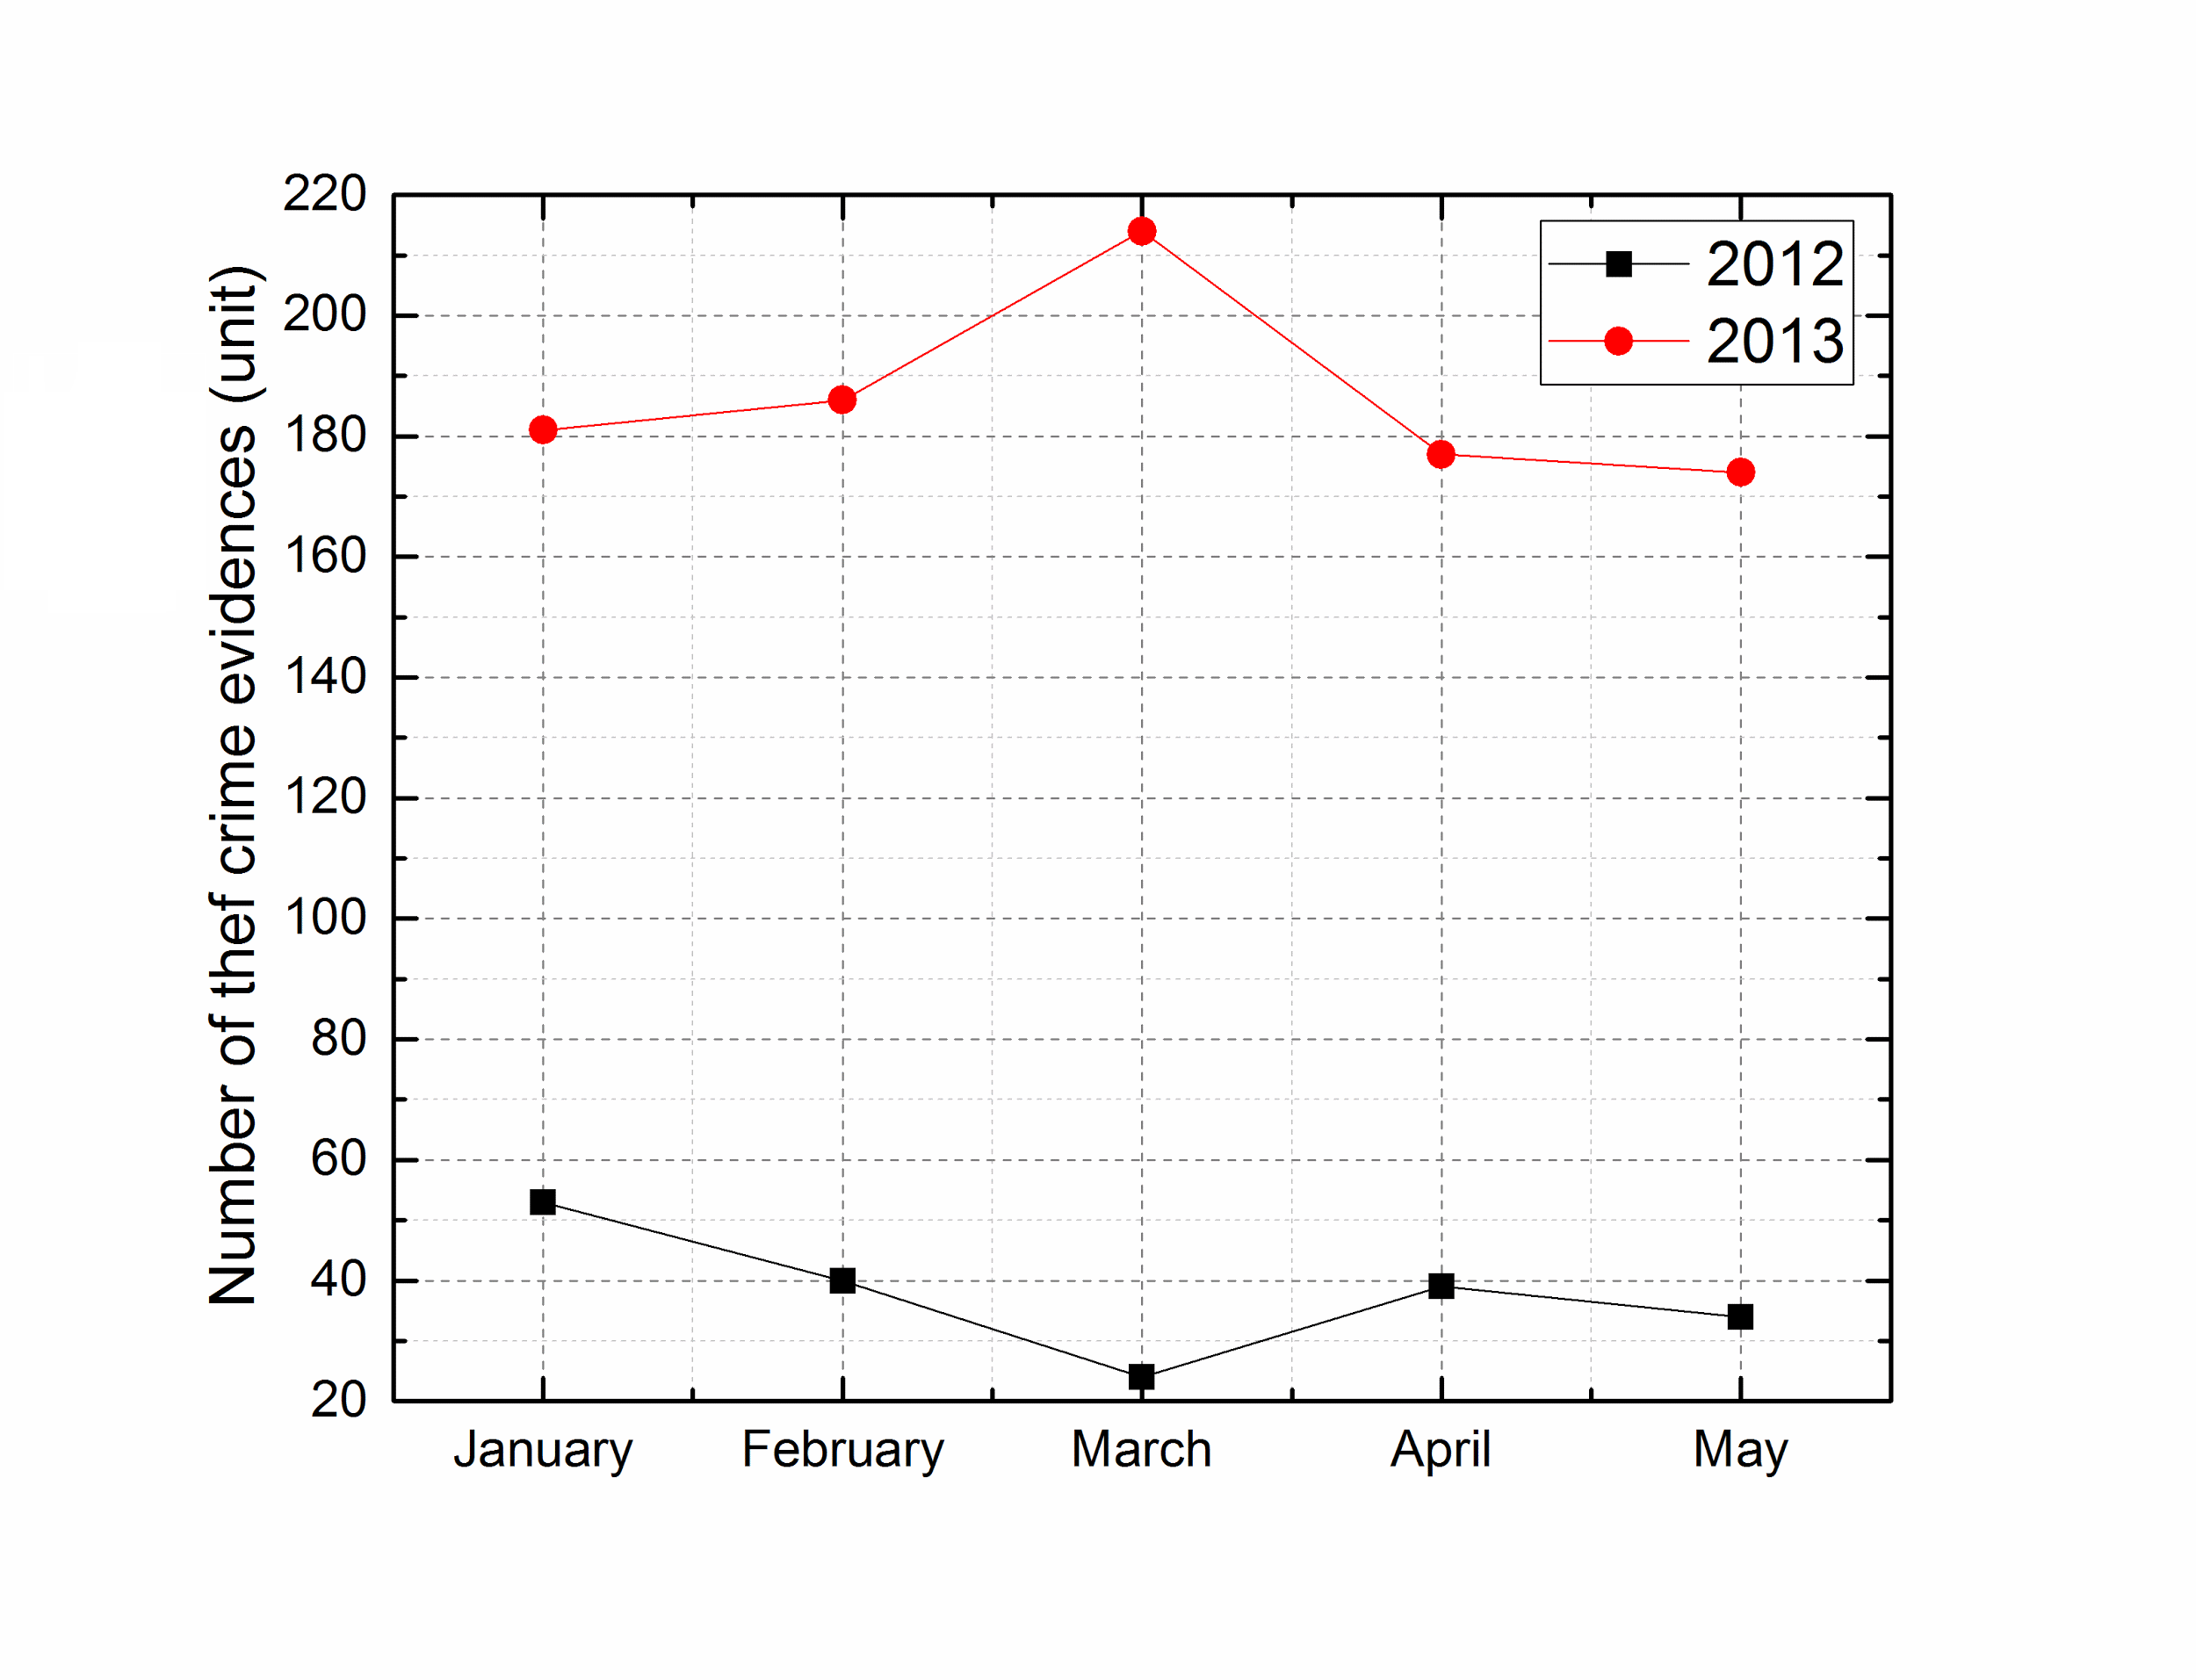
\includegraphics[scale=0.20]{Imagens/intro_fortaleza.png}
  	\caption{Numbers of witnessed crimes of theft in Fortaleza (2012 - 2013).}
  	\label{fig:fortal}
\end{figure}

In Natal, the Figure\ref{fig:natal} highlights the number of recorded events, based on information supplied by the Urban Public Transport Companies Union in the city of Natal - Seturn\footnote[3]{Urban Public Transport Companies Union in the city of Natal - SETURN. http://www.seturn.com.br. \textit{Accessed on December 1st , 2014.}}, which showed an increase of 198. 43\% in the rate of witnessed thefts from the year 2012 to 2013.

\begin{figure}[htb!]
	\centering
  	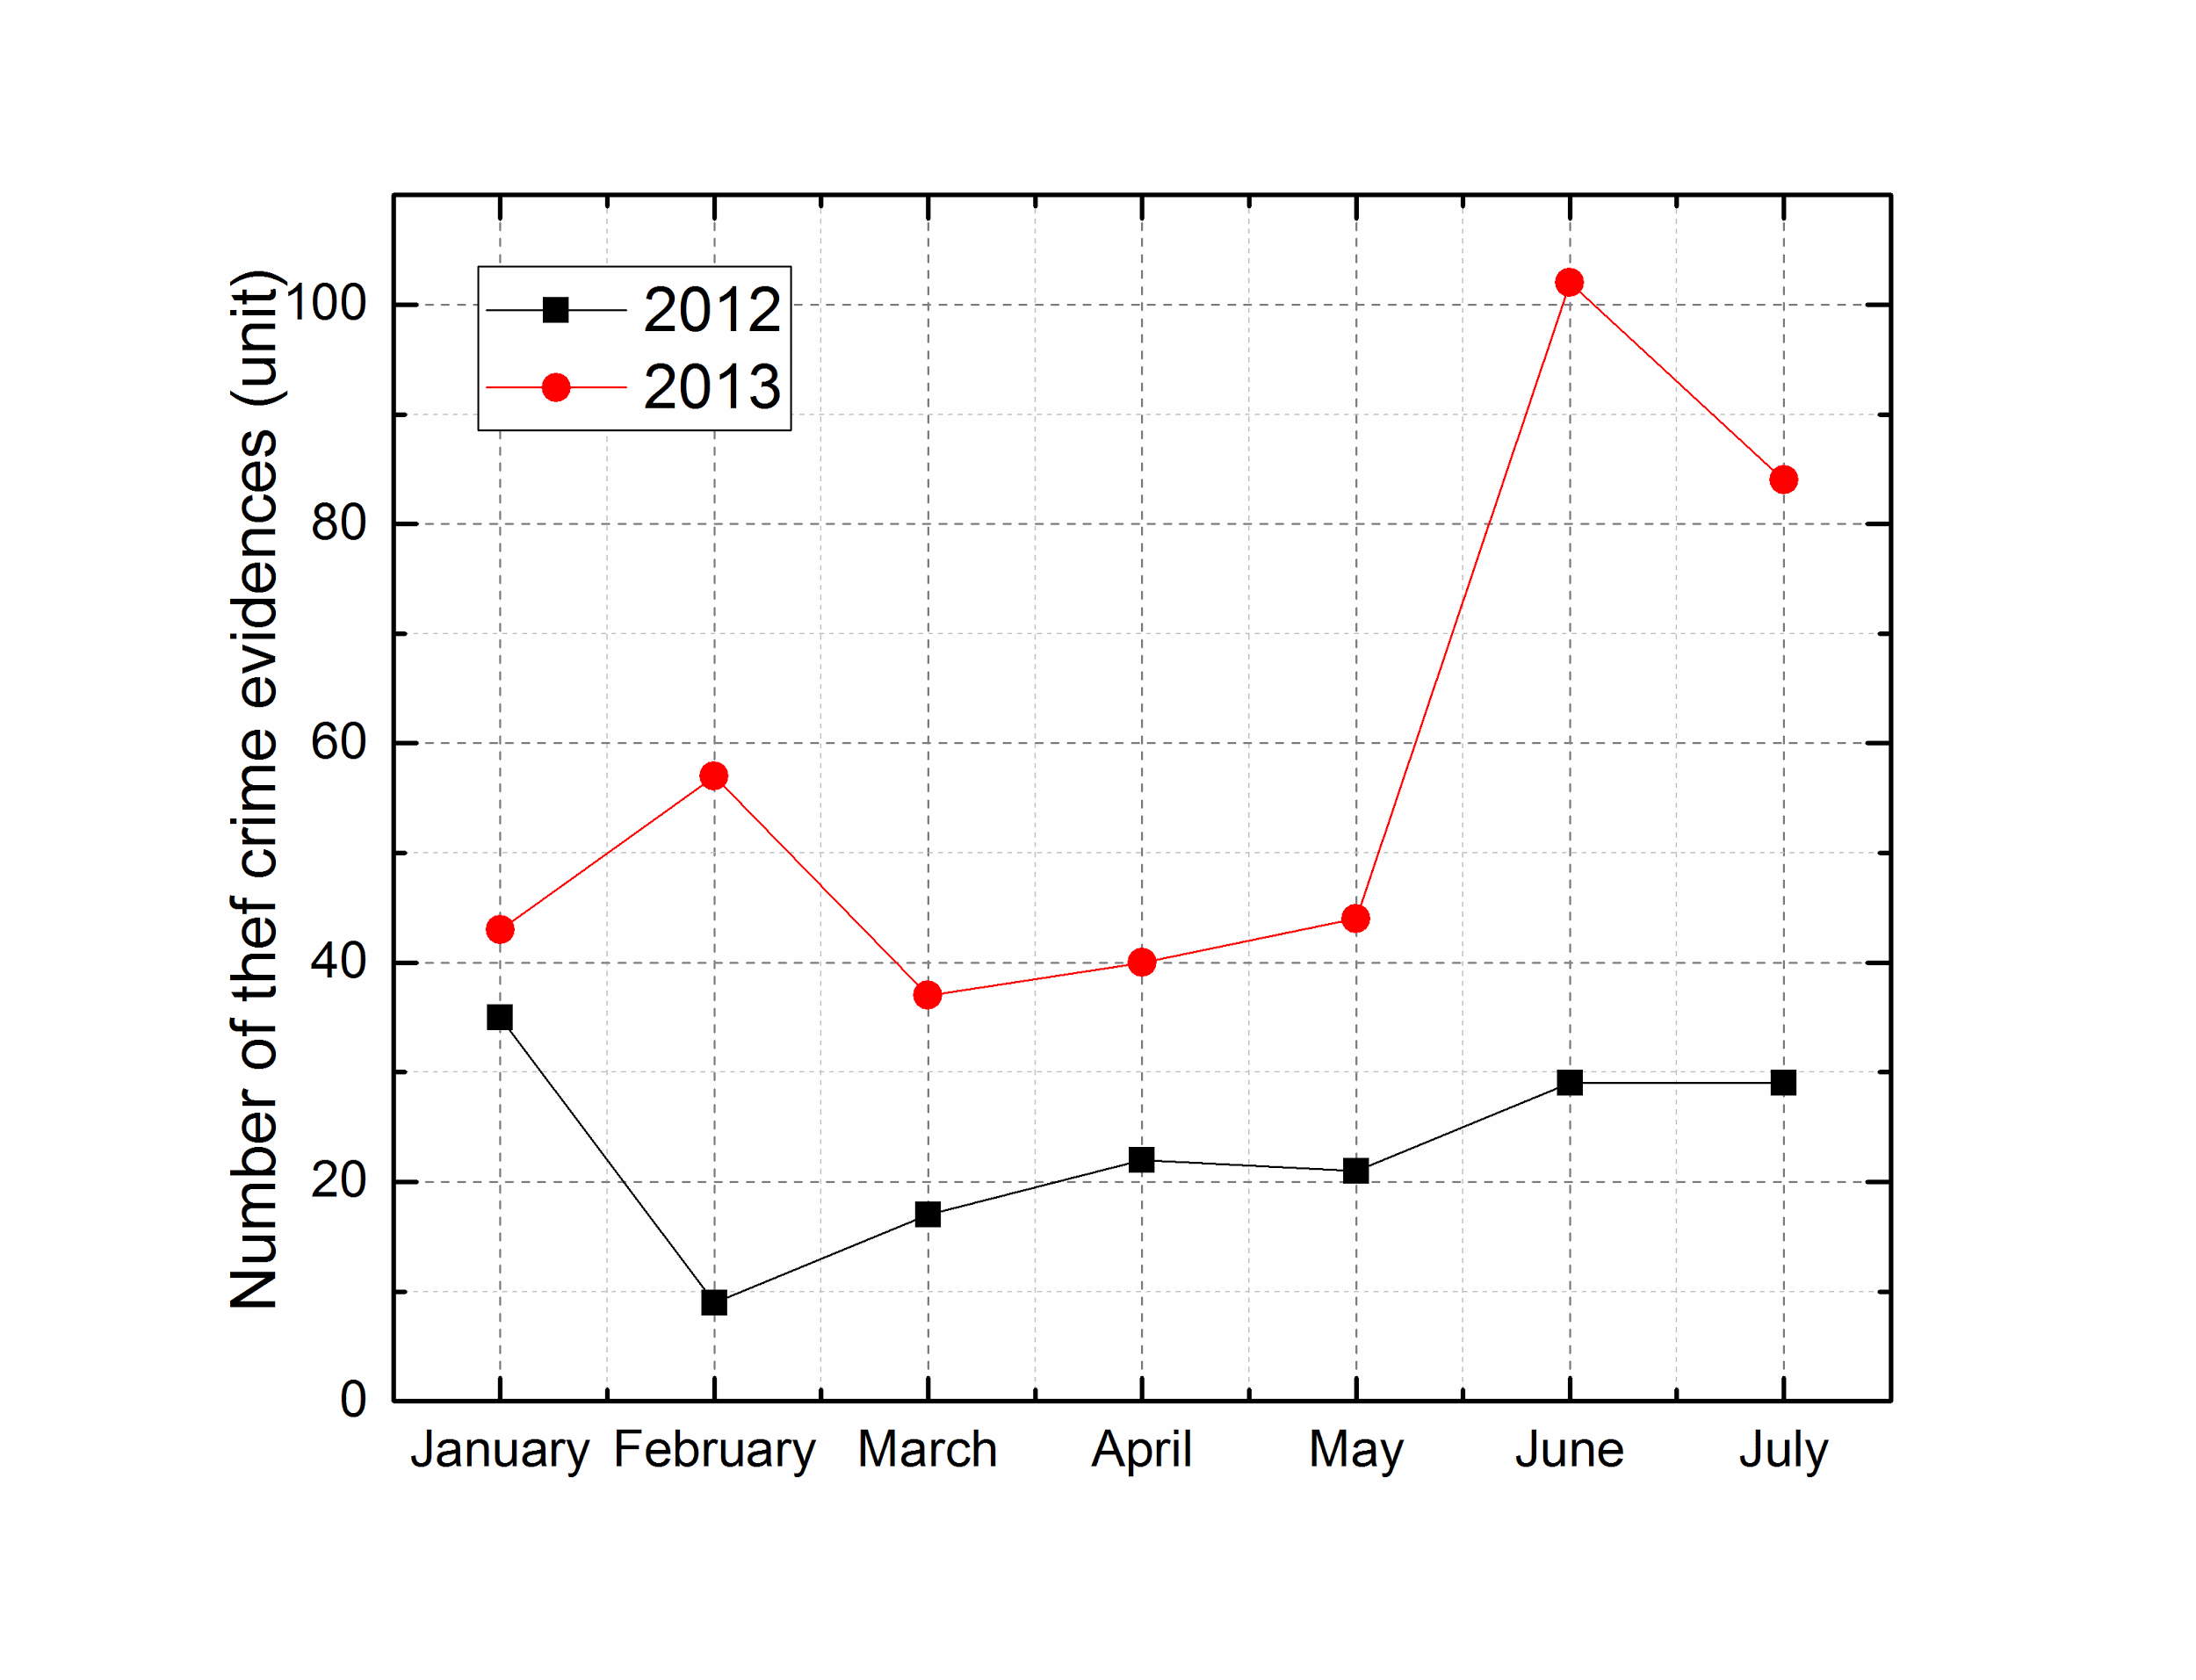
\includegraphics[scale=0.20]{Imagens/intro_natal.png}
  	\caption{Numbers of witnessed crimes of theft on buses in Natal (2012 - 2013).}
  	\label{fig:natal}
\end{figure}

The crimes on urban buses are mostly carried out with selected weapons (guns, sharp knives, etc.) which are primarily aimed at making the victim afraid, and if there is any resistance or sudden reaction on the part of the victim, the criminals often kill them in cold blood. This naturally increases the number of murders committed each year and makes Brazilian citizens feel extremely insecure. In light of this, transport safety in Brazil has become a real concern for the government and authorities, which are always seeking effective ways of eradicating (or at least alleviating) this social evil. The traditional model adopted by police authorities is 100\% reactive, since it relies on human intervention in the form of a request to assist the crime victim ( through the use of emergency call services, in-vehicle panic button systems, constant monitoring of surveillance cameras, and the like). 

However, the citizens (the users or drivers) are scared to make use of these available services because they might face retaliation from the criminals, and either be killed during the crime or later on in a revenge attack. As a result, over 90\% of the criminal offences are never detected by the police, and when criminals are arrested , only about 5\% to 8\% of the murderers are punished\footnote[4]{Nation Master - Brazil Crime Stats - http://www.nationmaster.com/country-info/profiles/Brazil/Crime. Accessed in December 10th, 2015.}; this leads to a feeling of impunity among the perpetrators.

Thus, it is essential to make use of to Information and Communication Technology (ICT) for event detection and subsequent response by means of automated systems. Smart Environments is a potential research field that leverages ICT to control urban violence \cite{Droege1997}. A Smart Environment can be characterized as a space with various network devices, which embeds processing power and sensing systems that cooperate with each other in assisting end-users to carry out their tasks more efficiently. 

A Smart Environment must be able to: (i) recognize the users and their circumstances; (ii) have a prior knowledge of the environment; (iii) produce new services in real-time in areas such as entertainment, security, health, housework, the work environment, information outlets, computing, communication, etc.; (iv) allow access to the services and features provided by a Smart Environment, and take account of the location and the time when the event occurs.

A successful applicability of Smart Environments is Smart Cities \cite{Komninos2006}, which refers to a physical environment and adopts an ultimate ICT embedded in the physical objects and environment in which we live. The field of Smart City is increasingly attracting the attention of the research community because it offers the prospect of deploying new and innovative ICT to boost urban services of a better quality, performance and interactivity since it is able to provision sustainable services, offer a better quality of life, and cater for both the public and the government.

Smart City services are multisector, and include the government, transport and traffic management, and the energy, health-care, water and sanitation sectors. Smart City applications are planned with the aim of improving the management of urban traffic and provides real- time responses to challenges.

Smart Surveillance\cite{barros2014} is a technology that adopts advanced processing techniques from the data gathered of surveillance subsystems (cameras and/or microphones) spread across a Smart City area. It seeks to process multimedia data obtained from a target monitoring zone, with the goal to detect/track security threats, such as a person's suspicious behavior or holding a dangerous object (knife or gun).

Smart Surveillance is mostly used in pedestrian zones (squares, sidewalks, shopping centers/banks, etc.), which have benefited from a high rate of crime incident detection, since the devices are installed in fixed places, and interconnected with standard communication techniques to the control center of the police authorities. Figure\ref{fig:fixed} provides an example of devices installed in fixed places and deployed through wide broadband in New York City - EUA.

\begin{figure}[h!]
	\centering
   	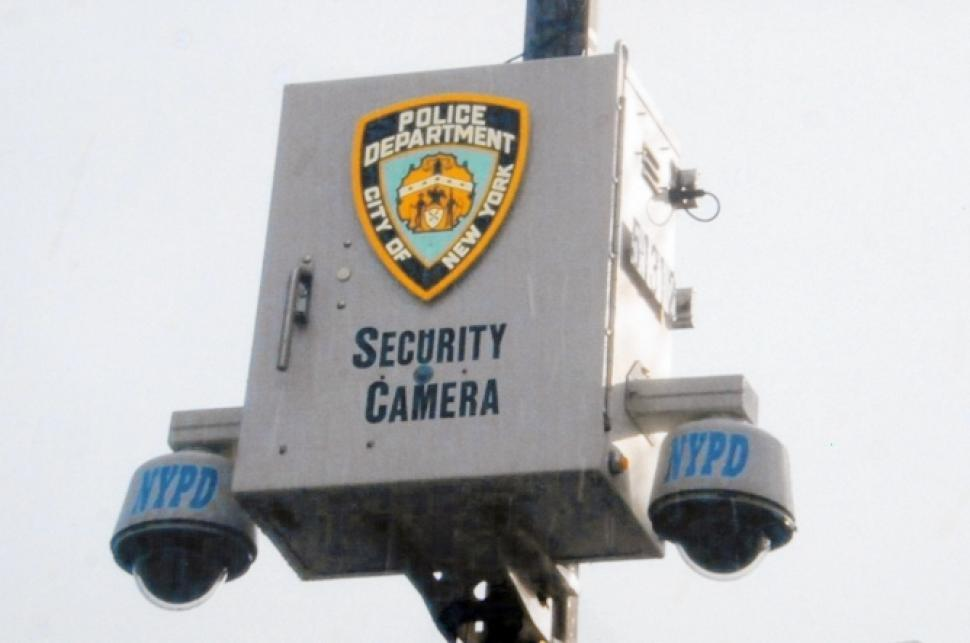
\includegraphics[scale=0.45]{Imagens/intro_fixed.png}
	\caption{Surveillance subsystem at a fixed place}
	\label{fig:fixed}
\end{figure}

Smart Transportation-Safety systems is an area in Smart Cities transportation\footnote[5]{Smart Transportation Alliance - http://smart-transportation.org/. \textit{Accessed in December 10th, 2015.}} that has attracted special attention in this study, because it involves innovative strategies for dealing with security threats in transport system. The main idea consists of exploiting an in-vehicle ICT that is integrated into other Smart City systems (control centers, intelligence authorities, cyber-physical systems, etc.) to reduce fatalities. 

In the scope of this dissertation, Smart Transportation-Safety is suited to the problem of crime incidents in Brazilian urban buses, since it provides ICT with the ability to cope with the violent incidents described above, and thus provide more safety for the public, as well as to drivers and conductors. With the support of specific multimedia sensors (e.g., video surveillance cameras and/or microphones) along with specific data analytics afforded by signal-processing techniques, it will be likely possible to automatically detect criminal threats at the time they are carried out, and hence trigger the most appropriate crime assist with more agility.

The dissatisfaction with the inefficient model currently adopted by police authorities in dealing with the crime incidents on buses, as well as the sharp rise in the re-incidence rates, forced urban bus companies constantly searching for alternative strategies that can assist in keeping criminals out of urban buses, or at least, hesitate before committing in-vehicle crimes. Initial measures have resulted in the installation of video cameras and GPS location sensors for the entire fleet, to allow the interior of the buses to be monitored (off-line), as well as to carry out tracking. 

With regard to video surveillance, the employers are in charge of analyzing the offline video files compiled by the cameras after an incident. This reactive scheme is naturally an inefficient way of avoiding an incident, especially fatalities, because it depends exclusively on humans operation to analyze the video for identifying events of potential security threats after physical occurrence, which may be doomed to failure in stressful conditions or other adverse factors. Rather than this, it would be helpful to enable the authorities to find out a criminal's identity and the way the crime has been committed.

Smart Transportation-Safety can be defined as a set of systems that feature computing capabilities to collecting, processing, and analyzing multimedia data for identifying events of potential security threats (e.g., robberies, fights, accidents, kidnappings, etc.) in the transportation service \cite{Anwar_Hossain}. Hence, Smart Transportation-Safety system is an asset for anticipated procedures, helping to mitigate the problem of crime on urban buses in an accurate and effective way, with more accuracy and agility in comparison to humans.

The evolution of multimedia signal processing techniques (audio, images and video), as well as pattern recognition, has led to the development of smart tools with great capacity for accurate detection and rapid decision-making \cite{Schonfeld2010}. Within the scope of this proposal, the target Smart Surveillance-based Transportation-Safety system is introduced as a system approach featuring a set of interworking and autonomous technologies. In another words, the targeted system must collect multimedia data through sensors in the bus cabin and processing them in real-time to automatically identifying events of potential security threats at bus cabins.

Other countries in Europe, Asia and North America have successfully adopted a similar technical form of Smart Surveillance-based Transportation-safety system and, achieved a reduction in crime\footnote[6]{Homeland Security News Wire - http://www.homelandsecuritynewswire.com/study-shows-surveillance-cameras-reduce-crime-some-cases. \textit{Accessed on December 10th, 2015.}}. Moreover, these  applications can be deployed to improve efficiency in prevention, affording a proactive approach. For instance, when an incident is detected, this application can embody capacities to alert the most appropriate authorities (e.g. a police vehicle with expertise on crime , which is located close to the area to deal with the incident by attempting to save the lives of the victims and punish the criminals.

To achieve this, the Smart Surveillance-based Transportation-Safety systems require the assistance of reliable communication technologies (broadband, mobile and quality guaranteed) and smart devices (sensors/actuators such as pan-tilt-zoom cameras). These are employed to support the following: a) mobility at high speed, b) a reliable transmission of data, c) the ability to keep the system available for ubiquitous access, and d) a means of switching/ moving directly to the Smart City zone to change the standard behavior. 

Thus the data produced will help both to assist in solving crimes and to prevent them by triggering reactive mechanisms which act as protective measures or, depending on the nature of the situation, can assist in saving victims.

On the basis of the the major concerns facing transportation-systems \cite{Karagiannis2011}, including scalability, ubiquitous access to sensory data, event processing overhead, and massive storage requirements, cloud Computing plays a key role in supporting several applications for high-performance and high-reliability perspectives \cite{Anwar_Hossain}. Cloud Computing is a successful concept that combines many fields of widely used computing paradigms to provide a service infrastructure that can reduce the costs of managing hardware and software resources \cite{Hayes2008}. 

In Smart Surveillance-based Transportation-Safety systems, cloud computing can benefit a powerful and scalable service infrastructure for large-scale storage, processing, and flexible dissemination of data/information. Cloud computing includes hardware, software systems, and the applications delivered as services over the Internet \cite{Xinhui2009}.

For the purposes of this work, we strongly believe that the combination of Cloud Computing with Smart Surveillance-based techniques is key enabler for an efficient Smart Transportation-Safety system, and will enhance public safety in Smart Cities by enabling the deployment of autonomous and real-time crime assist at bus service.

The resulting solution envisions to assist police authorities in finding the location of the crime, and thus getting the ability to respond to the incident efficiently (more agile and accurate). However, it is not a trivial task to deploy this system by facing the following challenges:

\begin{itemize}
\item Affording in-vehicle smart video surveillance subsystem with capacities to detect the occurrence of crime threats in real-time and with high-accuracy. To that, an efficient video processing algorithm, considering the high noise conditions on the bus cabin, plays a fundamental role on this process;

\item Deploying a cloud-enabled infrastructure, acting as a front-end between target vehicles surveilled and available crime assist units. The cloud infrastructure is envisioned to provision high-performance storage and processing (under smart computing design), as well as affording services with high-reliability, -accessibility and -availability;

\item Supporting event-driven mobile applications for use by crime assist unities. The event-driven mobile application is connected to the cloud service infrastructure to provide crime assist unities metadata (information about location, expertise, capabilities, etc.). Moreover, the cloud service infrastructure uses the event-driven mobile application to call crime assist, providing metadata about a detected security threat.

\end{itemize}

The challenges listed hereinabove are the basis for us to derive the motivation that is highlighted in the following section.

\section{Motivation}

To the best of our knowledge, there are no current works in the literature neither in the market that suit all the challenges described in the last section for affording efficient cloud-enabled Smart Surveillance-based Transportation-safety systems. This is the motivating factor that has driven this work and gives it global significance within both the research community and industry. Moreover, the resulting solution set out in this work is designed to help enhance aspects of public transportation-safety in Smart Cities. 

This is because, among other factors, it allows: (i) police authorities to respond to crime incidents with agility; (ii) city authorities to effectively plan city services and security; (iii) an improved quality of life for citizens and police authorities; (iv) plans for new applications to improve current strategies for public safety with proactive actions; (v) a greater degree of safety for the city.

\section{Objectives}

The main objective of this dissertation aims at evolving safety in transportation systems through exploiting emerging technologies in the research fields of ubiquitous and smart computing. The resulting approach includes designing a framework for loud Computing-assisted Smart Surveillance-based Transportation-Safety systems, and evaluating the architecture in a real testbed. In pursuing this goal, the specific aims that must be carried out to achieve the overall objective can be described as follows:

\begin{itemize}
\item Designing, implementing and evaluating a generic video processing mechanism for embedding the bus cabin system with smart surveillance camera subsystem. The smart surveillance camera is in charge for automatically detecting in-vehicle crime incidents, and sending the corresponding metadata to a cloud service infrastructure;
\item Designing, implementing and evaluating a cloud service infrastructure embodying applications that provision the following set of cloud services: (i) storage (for bookkeeping metadata of crime event detection produced by in-vehicle smart surveillance subsystems); (ii) multimedia processing (to classify the crime event detected by in-vehicle smart surveillance subsystems); and (iii) event notification (to select and call the best suited crime assist unit).
\item Designing, implementing and evaluating a mobile application that operates in a event-driven approach for lightweight behavior (allowing accessibility, survivability, best performance). The event-driven mobile application is the target for event crime notifications from the cloud service infrastructure, seeking to call crime assist;
\item Deploying the resulting framework on a real TestBed, for obtaining perspectives of accurate assessments and insights on the work proposal with use case;
\item Disseminating the obtained results in conference proceedings and journals that are certified and recognized by the Qualis\footnote[7]{CAPES/MEC. http://www-periodicos-capes-gov-br.ez18.periodicos.capes.gov.br/. \textit{Accessed on  January 30th, 2015.}} platform.
\end{itemize}

\abrv[3G -- Third Generation]{}
\abrv[CCTV -- Closed Circuit Television]{}
\abrv[CPU -- Central Processing Unit]{}
\abrv[DCD -- Dominant Color Descriptor]{}
\abrv[DOT -- Dominant Orientation Templates]{}
\abrv[EC2 -- Elastic Compute Cloud]{}
\abrv[EHD -- Edge Histogram Detector]{}
\abrv[FP7 -- EU Framework Program 7 for Research and Innovation]{}
\abrv[GPS -- Global Position System]{}
\abrv[Haas -- Hardware as a Service]{}
\abrv[IaaS -- Infrastructure as a Service]{}
\abrv[ICT -- Information and Communication Technology]{}
\abrv[IoT -- Internet of Things]{}
\abrv[IP -- Internet Protocol]{}
\abrv[IR - Infra Red]{}
\abrv[ISIS -- Intelligent Sensor Information System]{}
\abrv[JNI - Java Native Interface]{}
\abrv[NIST -- National Institute of Standards and Technology]{}
\abrv[PaaS -- Platform as a Service]{}
\abrv[PC -- Phase Correlation]{}
\abrv[PLS -- Product Lines Software]{}
\abrv[QoE -- Quality of Experience]{}
\abrv[QoR -- Quality of Recognition]{}
\abrv[QoS -- Quality of Service]{}
\abrv[RF -- Radio Frequency]{}
\abrv[S3 -- Simple Storage Service]{}
\abrv[SaaS -- Software as a Service]{}
\abrv[SIFT -- Scale-Invariant Feature Transform]{}
\abrv[SETURN -- Urban Public Transport Companies Union in the city of Natal]{} 
\abrv[SINDIONIBUS -- Urban Public Transport Companies in the Satate of Ceara]{}
\abrv[SLA -- Service Level Agreements]{}
\abrv[SSL -- Secure Socket Layer]{}
\abrv[ADABTS -- Automatic Detection of Abnormal Behaviour and Threats in crowded Spaces]{}
\abrv[LOTUS -- Localization of Threat Substances in Urban Society]{}
\abrv[IMSK -- Integrated Mobile Security Kit]{}



 % Introdução
	
	% Capitulo 2: Segundo capítulo (arquivo Includes/Capitulo2.tex)
	% Capítulo 2
\chapter{Theoretical Background}

This chapter discusses factors related to Ubiquitous Computing, Cloud Computing and the technologies derived from them, as well as Ubiquitous and Smart Surveillance.

\section{Smart Cities}
Smart Cities is a significant paradigm for proposing and deploying various innovative technologies to make cities smarter and improve people's quality of life\cite{Pribyl2015}. The evolution of the Smart City concept is shaped by a complex mix of technologies, social and economic factors, governance arrangements, and policy and business drivers. The implementation of the Smart City concept, thus follows various paths depending on each city's specific policies, objectives, funding and scope. 
According to \cite{Schaffers2011}:

\begin{quotation}
\textit{"...\\A city may be called "Smart" when investments in human and social capital and traditional and modern communication infrastructure fuel sustainable economic growth and a high quality of life, with a wise management of natural resources, through participatory governance."\\...}
\end{quotation}

On the basis of cited definitions of smart cities, a set of factors can be enumerated that comprise the activities of autonomous, independent and aware citizens. In Figure \ref{fig:smart} the correlated features of smart cities are shown, which underlie the "smart" combination of endowments and activities of autonomous, independent and aware citizens.


\begin{figure}[htb!]
  \centering
    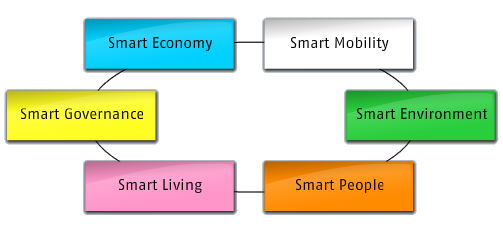
\includegraphics[scale=0.99]{Imagens/cap2_smarcite.png}
    \caption{Characteristics of Smart cities.}
    \label{fig:smart}
\end{figure}


Smart Mobility is a key feature in this proposal since its principles include "Sustainable, innovative and safe transport systems".
The availability of a secure, efficient and affordable transport system is one of the defining goals of any smart city. However, many cities today are facing challenges when implementing comprehensive "smart mobility" programs, including those that are secure and deal with a legacy infrastructure. The proposal outlined in this study was designed to improve the prospects of Smart Mobility.

\section{Ubiquitous Computing}

The constant technical advances in communication and computing have given rise to a scenario which a short time ago was only just being glimpsed by Pervasive Computing, and this means that computing is now a common feature of people's routine activities, and before long will form a part of our everyday lives. Furthermore, forecasts predict that microprocessors will become smaller and smaller and will soon be cheap enough to be embedded in digital devices, electronic appliances, everyday objects and clothes, as well as in cars.

This scenario is regarded as the new paradigm of the Century\cite{943998} \cite{Saha2003}  or the third wave of computing. It is enabling the physical world to be combined with the world of information and provides a wide range of services and ubiquitous applications such as target users, machines, data, applications, and various objects in physical space, so that they can interact with each other in a transparent way \cite{Ranganathan2005}. 

Hence, technology is gradually moving toward a world of ubiquitous computing, or incrementally having to rely on a set of heterogeneous devices to support a growing range of applications that are suited to this scenario.
According to its creator Mark Weiser, \textit{"deeper technologies are those that disappear"} \cite{Weiser1999}. From this perspective, Ubiquitous Computing is seeking to include computing in the physical world of the user, by allowing it to concentrate on the tasks that have to be accomplished and not just the tools that are needed for this.

According to \cite{Hansmann2001} ubiquitous systems are based on at least five principles:
\begin{itemize}

\item Diversity: This characteristic is related to devices, especially different kinds of computers in terms of specific task performance. For example, while a tablet is the most suitable device for viewing content, a notebook might be more appropriate for writing long texts;

\item Connectivity: The presence of different devices performing specific tasks, requires a high connectivity, to maintain cooperation and mobility among its users;

\item Decentralization: Despite the presence of servers, cooperative and distributed environments require decentralization, and it is worth noting that a flow of information is needed to be transmitted to the hosts, regardless of the particular characteristics of the environmental devices. Decentralization and diversity are accompanied by information synchronization, since it is essential for this system to be regularly updated in all the devices to maintain data consistency;

\item Invisibility: This supports the idea that technology in particular is a part of the environment. Computers offer a good means of achieving this and can become essential tools for interpreting our activities, since they are spread throughout the environment and have become present and imperceptible;

\item Context Awareness: ubiquitous applications must act in a desired context or situation that is chosen by the user so that they can become transparent. Applications provide their best performance when the users can understand the context in which they live and act on this information;

\item Proactivity: the ubiquitous software must be programmed to predict events and react without human interaction. 
\end{itemize}
Moreover, it is important to ensure that they do not take action on the basis of misinformation.
Although there have been numerous attempts to develop ubiquitous applications, the question of their practicality is still an open question, but this is not a major issue and beyond the scope of this work. On the basis of these principles, the concept of Ubiquitous Surveillance arises \cite{Orwel42} as a sub-area of Ubiquitous Computing that is concerned with surveillance. This work envisions that Ubiquitous Computing concepts should mainly provide invisibility, decentralization and connectivity among other benefits.


\section{Ubiquitous Surveillance}

Given the complexity of the features of Ubiquitous Computing, Ubiquitous Surveillance is a science that is geared towards monitoring citizens for their personal safety, and can also be applied in the area of public health, for example, to control epidemics, as well as in the fight against terrorism. This is achieved by obtaining valuable information from fixed cameras in public places or even micro air vehicles that operate in a semi-autonomous manner, as shown in \cite{Nardi2006}.

Among important studies that have put forward suggestions for improvements in ubiquitous surveillance systems, the work of \cite{Chen2009} should be mentioned. In this, the authors designed a multicast overlay in IP (Internet Protocol) networks, which offers the prospect of not only increasing the stability of ubiquitous surveillance services, but also providing a dynamic load balancing, since there is a wide bandwidth for end-user applications. Apart from making technical improvements, the work proposed by \cite{Wang2008}, applies an encryption algorithm to ensure the information security and privacy of those involved.

This and other proposals have focused on the evolution of image acquisition techniques in IP networks; however, they leave video analysis to the end-user, which means they are ubiquitous monitoring systems that are completely dependent on repetitive human endeavor. This fact makes them unviable for current surveillance systems, first because of the vast amount of data generated by the wide range of devices and second on account of the limited number of professional security experts that have the necessary skills to predict and detect these events. Moreover, the quality of life falls exponentially as these specialists have to be aware of multiple simultaneous monitoring systems throughout the working day.


\section{Smart Surveillance}

With regard to disability surveillance which is currently only carried out by human means, there are several research papers aimed at automating  ubiquitous surveillance  Some of them are listed in \cite{Sodemann2012}.  These works essentially use all the features combined with extraction techniques for machine learning and these are either Supervised or Unsupervised. Figure 5 shows a diagram of the intelligent monitoring targets and their interrelationship.

Thus the assumptions made about effective automatic surveillance are formed on the basis of a particular target environment. With the aid of this concept, the purpose of this study is to create a mechanism able to support smart surveillance algorithms by providing ubiquitous access, augmented processing power and seamless operations. Thus the analysis can show the objects used for these criminal acts.


\begin{figure}[htb!]
  \centering
    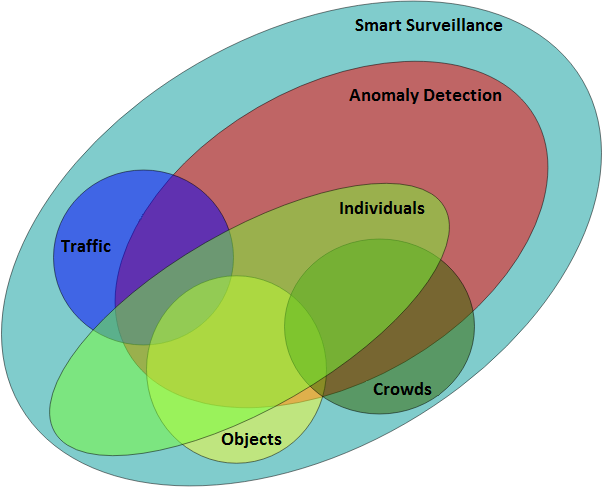
\includegraphics[scale=0.50]{Imagens/cap2_diagram.png}
    \caption{Venn Diagram - Smart Surveillance Targets.}
    \label{fig:targets}
\end{figure}

The formulation of an automated monitoring approach requires a starting- point that provides definitions and assumptions about the application being targeted. In the case of the proposal in question, making these assumptions is not an easy task because it entails a shifting environment and also the crimes may be committed in different ways. However, crimes committed in the vehicular environment are generally carried out with threatening weapons. In view of this, there are three measures that can be taken to make smart surveillance more effective, which are as follows: 

\begin{itemize}
\item Look for  dangerous objects in the environment, since they  are  less often found  than normal objects;
\item Be aware that  dangerous objects have significant features that make them  different  from normal objects;
\item Note that any particular objects that  appear on the scene may have some meaning. For example, if someone waves a gun in a bus, it can be assumed that a crime is bound to take place.
\end{itemize}

These measures make it clear how the tool should be employed. This is through video streaming which can benefit intelligent surveillance applications.


\section{Cloud Computing}

The concept of cloud computing has emerged from the need to allocate computing resources dynamically, and makes it possible to centralize scalable and secure processing, with sufficient momentum to support various types of applications. Vehicular applications can meet these requirements since they include even more dynamic environments. 
According to \cite{Buyya2009}:

\begin{quotation}
\textit{"...\\Cloud is a type of parallel and distributed system consisting of a collection of interconnected and virtualized computers that are dynamically provisioned and presented as one or more unified computing resource(s) based on service-level agreements established through negotiation between the service provider and consumers.\\..."}
\end{quotation}


On the basis of this definition, Cloud Computing technologies are adopted in this work to increase its processing power, seamless operations and ubiquitous access. All of its known benefits and characteristics will be described below in the next sub sections.

\subsection{Cloud Components}

The three main components of cloud computing are Clients, Data Center and Distributed Servers\cite{Velte2009}.
Clients are the devices with which end-users interact to manage their information on the cloud. Clients might be smart phones or computers without a hard disk (a thin client) or a regular computer (a thick client). A thin client is generally a web browser like Google's Chrome or Mozilla's Firefox. 

A Data Center is a collection of servers that contains the application subscribed by the customers who can access it via the Internet. Many virtual machines can execute tasks simultaneously on a single physical server, also known as the host. The number of virtual servers that can exist on a physical place depends on its size and speed and what applications will be running on the virtual server \cite{Velte2009}. 

The servers are placed in geographically dispersed locations so that they can provide available servers that are more reliable(Distributed Servers). This means that if one server fails, the service can be continued by another. They also increase scalability. If the cloud needs more hardware, it is not essential to deploy more servers only in the data center. They can be added at another site or be simply made a part of the cloud \cite{Velte2009}.

\subsection{Features of Cloud Computing}

According to the National Institute of Standards and Technology - NIST, there are five essential characteristics for cloud computing\footnote[8]{http://www.nist.gov/}. Each is described below in simple terms:

\begin{itemize}

\item Measured Service: Cloud Services are controlled and monitored by the cloud provider. This is crucial for billing, access control, resource optimization, capacity planning and other tasks;

\item On-Demand-Self-Service: The consumer can use cloud services as needed without any human interaction with the cloud provider; 

\item Ubiquitous Network Access: The cloud provider's capabilities are available over the network and can be accessed through standard mechanisms by both thick and thin clients; 

\item Resource Pooling: this allows a cloud provider to serve its consumers via a multi-tenant model. Physical and virtual resources are assigned and reassigned in accordance with consumer demand. The customer generally has no control or knowledge over the exact location of the provided resources but may be able to specify the location at a higher level of abstraction (e.g., country, state, or data center).

\end{itemize}

\subsection{Service Models}

On the basis of the NIST Cloud Computing definition, there are three service models, widely known as "textit{as a service}". These are described below:

\begin{enumerate}

\item Software as a Service (SaaS) - In this model, an application is hosted as a service to the customer who accesses it via the Internet. This spares the customer the headache of having to update and maintain the software. Some of the benefits are as follows:

\begin{itemize}
\item Greater reliability since if one server fails another server will replace it;
\item Security implemented by Secure Socket Layer (SSL) allows customers to reach their application securely;
\item Due to an increase in bandwidth, an organization can access its application with less latency and at a higher speed.
\end{itemize}

\item Platform as a Service (PaaS) - Supplies all the resources required to build applications. There is no need to download or instal software. This is also known as cloudware. The services provided by PaaS are application design development, testing, deployment and hosting. Google AppEngine and Microsoft Azure are two examples in this category. Some of the benefits of PaaS include: 

\begin{itemize}
\item It enables geographically-isolated development teams to work together by merging web services from multiple sources;
\item An ability to make cost savings by using built-in infrastructure services for security, scalability, and failover, rather than having to obtain and test them separately;
\item It makes cost savings by using higher-level programming abstractions.
\end{itemize}

\item Infrastructure as a Service (IaaS) - This offers the hardware which the application provided by SaaS and PaaS can work on. It is also known as Hardware as a Service (HaaS). The physical assets provided by IAAS are storage space, network equipment and computing power. The infrastructure provided can be scaled up or down depending on the possible resource needs. Furthermore, multiple tenants can share the equipment at the same time. The resources are usually billed on a utility computing basis, which means that providers charge the clients on how many resources they use. Amazon EC2 (Elastic Cloud Compute), Amazon S3 (Simple Storage Service) are examples of IAAS. The components of IAAS include:

\begin{itemize}

\item \textbf{Service Level Agreements (SLA)} - This is an agreement between the provider and client, that guarantees a certain standard of performance from the system;

\item \textbf{Computer hardware} - These are the features that have resources which will be rented out. The service providers often have this set up as a grid for easier scalability;

\item \textbf{Network} - This includes hardware for firewalls, routers, load balancing, and so on;

\item \textbf{Internet Connectivity} - This allows clients to access the hardware from their own organizations;

\item \textbf{Virtualization} - This enables clients to run the virtual machines with their own settings and also clone them as needed;

\item \textbf{Utility Computing} - this is set up to bill customers and is based on how many system resources they use.
\end{itemize}
\end{enumerate}
\subsection{Observations on Cloud Computing}

Cloud services are popular because they can reduce the cost and complexity of owning and operating computers and networks. Since cloud users do not have to pay for information technology services, purchasing hardware, or buying software licenses, the benefits are low up-front costs, a rapid return on investment, rapid deployment, customization, flexible use, and solutions that can make use of new innovations. In addition, cloud providers that are specialists in a particular area (such as e-mail) can offer advanced services that a single company might not be able to afford or develop. Some other benefits to users include scalability, reliability, and efficiency. Scalability means that cloud computing offers unlimited processing and storage capacity. Figure  shows a diagram of cloud computing and its inherent benefits.


\begin{figure}[htb!]
  \centering
    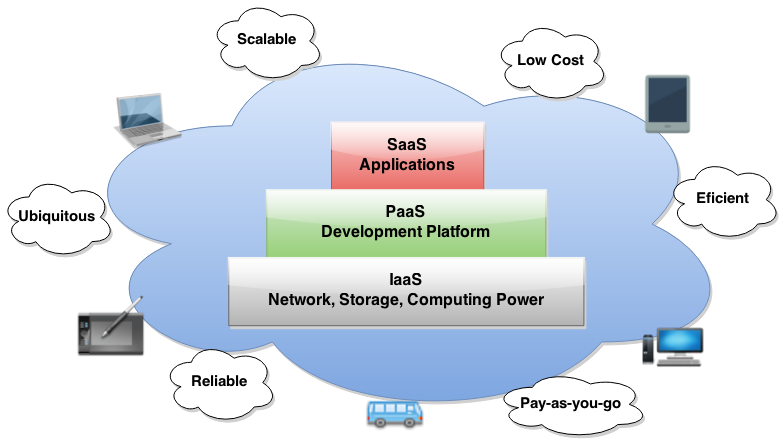
\includegraphics[scale=0.50]{Imagens/cap2_cloudremark.png}
    \caption{Diagram of Cloud Computing.}
    \label{fig:smart}
\end{figure}

The cloud is reliable in that it provides access to applications and documents anywhere in the world via the Internet. Cloud computing is often considered efficient because it allows organizations to free up resources and thus be able to focus on innovation and product development. 

For the purposes of this work, it is necessary to design and implement a cloud service for the proposed vehicular public safety application, as well as other areas that can make use of the information acquired by cloud. 

\section{Conclusion}

In this chapter, there has been a general overview of the technologies related to this work and its main concepts . In the next Chapter, there will be a detailed account of the "Related Works". % Fundamentação Teórica
	
	% Capitulo 3: Terceiro capítulo (arquivo Includes/Capitulo3.tex)
	% Capítulo 3
\chapter{Related Work}

In traditional surveillance computing systems, specific service applications are deployed as a way to help detecting potential crime events, as well as triggering crime assistance, with more agility and accuracy than when carried out only by humans. As a consequence, these systems demand a huge amount of resources (e.g., processing, storage and networking) for affording multimedia data transmissions to remote systems that will execute on them appropriate real-time analytics. Therefore, such infrastructures are very costly, by requiring to embody high-performance and robust servers to host very specific service applications with reliable capabilities to cope to the rigorous system and scenario demands. 

The present dissertation aims at evolving the scenario described hereinabove, with the main goal to enhance safety in transportation system through exploiting emerging technologies in the research fields of ubiquitous and smart computing. We claim that the integrated use of smart surveillance techniques and cloud computing play a key role to afford the target smart transportation-safety system. In regards to smart surveillance, the goal is to produce data (video, image and/or sound) from multimedia sensor devices, and deploy specific algorithms (at the device or at remote systems) to afford automatic real-time detection of safety event. In what concerns cloud computing, this largely-used technology provides high resource (processing, storage, etc.) availability, service reliability and availability as core competitiveness and advantage, specially in mission critical use cases. 

With the perspective to efficiently achieve efficient service platform for smart transportation-safety system, we believe that following key design principles must be met:

\begin{itemize}
\item Agile and accurate detection and classification of crime events in real-time based on video surveillance devices;
\item Heavyweight service applications provisioned at the cloud, in order to afford high-performance hub-service and ubiquitous access;
\item Distributed service approach, for scalability perspectives;
\item Event-driven mobile applications, for allowing lightweight computing and energy sustainability at the mobile devices in possess by crime assist team; 
\item Raw video or sensor data storage at the cloud.
\end{itemize}

This Section lists the most relevant related works within this dissertation's field of study. Analysis over corresponding concepts, characteristics, architecture and others aspects are provided taking into account the key design principles that has being outlined above for affording the design of efficient smart safety-transportation systems. The list of related works comprises attempts that are available in both the research community and in the market.

\section{Research works}

With regards to the efforts applied by the research community in the field of smart transport-safety systems, a cloud-capable video surveillance approach is proposed in\cite{Rodriguez2012}. In this work, the main idea consists in transmitting multimedia data of video surveillance cameras, along with the linked metadata, to the Amazon's S3\footnote[9]{Amazon's S3. Available at: https://aws.amazon.com/pt/s3/. \textit{Accessed on December 8th, 2015.}} cloud service. In order to prevent video quality degradation that may occur during the data transmission to the remote cloud storage service, authors propose to carry out optimizations in the video taking into account current network conditions. Although an interesting proposal, authors rely on a questionable assumption to afford the optimizations, which means the accessibility of the required information about the current network conditions. For that, it is necessary to deploy their own network infrastructure, in order to make possible gathering all required network measurements. In third-party network infrastructures regularly used in smart city systems (e.g., cellular, telecom, cable, etc.) this measurement will be not possible by policy restrictions of the net providers, which will turn the proposal unfeasible. 

A safety system, leveraging smart video surveillance technology, is presented in \cite{salmane2015}. The work addresses to evaluate abnormal events in urban scenarios for detecting safety threats. Four fixed scenarios are studied, treated and assessed. \textit{Vehicle Stopped}, \textit{Vehicle Zigzagging}, \textit{Queuing Across the Rail} and \textit{Fall of a Pedestrian}. For each scenario, a Hidden Markov Model is developed with the aim to estimate trajectories and then detect dangerous situations at a road.  The proposal leverages the Wireless Access for Vehicular Environment (WAVE) networking technology to alarm approaching users. Although interesting, cloud computing technology is not used in the proposal architecture. 

\cite{Moniak2007} proposes a transmission system to connect urban bus safety systems and corresponding control centers. In this work, the issue in offering high data rates in mobile networks, especially in vehicular networks, are addressed. A complete transmission chain developed for a robust and high data rate wireless link is used to transmit audio and video streams between an Urban Bus and a Control Center for safety applications. A real transmission system has been built on the basis of the simulation and experiments are made in real testbed to evaluate proposed system. The work focus exclusively in affording secure data transmissions among Urban Bus and a Control Center, missing neither smart surveillance nor cloud computing.  

An agency-like prototype model for cloud-based smart surveillance applications is proposed in \cite{FANG2013}, which is based on the design of hardware monitoring with a failure-handling mechanism. The authors design a software that promises to share infrastructure in building smart surveillance applications through cloud. The main idea consists in allowing to both submit and schedule data flow (audio or video) provided by any language, using a single channel. Although intercommunication details are considered in this work, details for automated data evaluation are missing. These features are already envisioned by the \textit{IaaS} cloud Computing paradigm. Similarly, a platform based on Apache Hadoop2 is proposed in \cite{Xiang2013}, which seeks to handle overloads for video conversion/compression and storage tasks. Once video quality is an essential feature in video automated evaluation, the compression technique that is deployed for this work is not suitable for keeping evaluation algorithms working properly.

\cite{Wen2010} proposed a cloud-based framework for surveillance which sends all the collected image frames to the cloud in real time for processing. In this work, the authors design the  WAMP - \textit{Worker Agent Messaging Protocol}, a third-party communication protocol that operate amongst clients and worker agents. The WAMP is based on a \textit{request/response} messaging approach, with following similar structure: the message header contains the description of the demanding operation (e.g. calculation of the topology between two cameras); and the message body is populated with the parameters or data required to complete the target operation (e.g. the labels of two target cameras). The operational messages sent by agents are notably expensive in this approach, and overloads the system exponentially with the increasing number of monitoring points, which is undesirable for large-scale environments.

A set of Streaming-based proposals are highlighted below. In the work carried out by \cite{Cheng2014}, a software architecture for audio transmission to network cameras is presented. This work proposes audio integration between heterogeneous camera devices in order to improve object detections, as example the author cited a gunshot sound, to facilitate detection of a dangerous situation.  Moreover, \cite{Paul2013} proposes a client-server surveillance solution, in which images gathered from android device camera are transmitted towards cloud service applications for remote detection and recognition tasks. A cloud-based smart surveillance framework for robots is introduced in \cite{Yang2015}, that leverages cloud computing services in ways to extend both computing and storage capabilities of the local robots. All the data collected by the robots are saved in the cloud, assuming that all required computing resources are allocated in an on demand way. Since robots are not prepared to locally process the video data, the data must be streamed to the cloud infrastructure for video processing. 

All works described in the previous paragraph share the same key need for available broadband connectivity to allow video data transport with high quality, otherwise the accuracy in detection and recognition tasks carried out at the cloud cannot be assured. This performance issue is raised by the streaming-based principle adopted to afford multimedia data transmissions to remote systems hosting the targeted processing service application, that is in charge to detect and react on the crime event. Furthermore, streaming-based surveillance applications are subject of video quality degradation that may be imposed by the conditions of the available networking technology, in terms to instability and/or overload, that is emphasized in wireless scenarios and becomes worst in mobile ones (focus of this work). 

\section{Market-Available Solutions}
 
The smart surveillance market is becoming more and more popular, and increasing day by day its popularity and penetration in the society by the availability of low-cost cameras embodying powerful image processing algorithms. 
Usually, a home "smart" camera is able to instantaneously alerting the owners of any movement it detects,  exploiting Internet connectivity through a smartphone, computer, tablet or smart Watch via local Wi-Fi to send email and/or text message over the cellular infrastructure (if it is the case). Although very useful when the detection corresponds to on-going critical security threats (intruder), this service can become a hassle when the notifications are constantly sent for no significant reason (e.g., upon detecting an inoffensive
 butterfly or even pet). The Netatmo\footnote[10]{Netatmo. http://www.techtimes.com/articles/122385/20160108/netatmo-presence-smart-surveillance-camera-can-tell-if-it-s-an-intruder-or-your-cat-lurking-outside-your-home.htm. \textit{Accessed on November 2nd, 2016.}} Presence Smart Surveillance Camera is an example. Although providing capabilities to differentiate between a person and an animal, such smart cameras category are unsuitable for the target scenario of this work. Smart surveillance transportation-safety, quick detection of crime objects with high accuracy under unpredictable motion conditions and different noising (e.g., luminosity) is strongly required due to its mission critical characteristics. Other video surveillance service category available in the market is focused on allowing access to private security system (at home, buildings, companies, etc.) quickly and easily, avoiding complicated settings (e.g., dynamic DNS) for forwarding. 
The list of such surveillance services include the IEVDA\footnote[11]{IEVDA. https://www.iveda.com/technology/iveda-cloud-whitepaper/. \textit{Accessed on December 12th, 2015.}}, Skywatch\footnote[12]{Skywatch. http://www.marketwired.com/press-release/skywatch-inc-announces-smart-video-surveillance-cloud-service-at-cloud-expo-2015-2029404.htm. \textit{Accessed on December 12th, 2015.}} and Intelbrascloud \footnote[13]{Intelbrascloud. http://www.intelbrascloud.com.br. \textit{Accessed on December 12th, 2015.}}, and many others. On these set of application, a cloud infrastructure enables ubiquitous access to real-time content of pre-configured surveillance cameras. The cloud infrastructure is only in charge to store the video produced by the surveillance cameras, whereas users can access through web page or mobile application. Advanced video processing support, to detect security threats for instance, is missing on this set of safety applications. 

Brickcom\footnote[14]{Brickcom. http://www.brickcom.com/. \textit{Accessed on December 12th, 2015.}} provides solutions based on IP cameras. This company's approach provides a solution only for a very specific use case, and it is not suitable for generic use. Moreover,  Brickcom cloud employment allows for both storage and streaming use. In the same way, Smartvue\footnote[15]{Smartvue - Cloud video Surveillance Solutions. http://smartvue.com/index.html. \textit{Accessed on December, 12th, 2015.}} is yet another cloud-based video surveillance market solution that offers a storage service and mobile monitoring application for end users to access their private systems.

The ARUOM Safety Technology \footnote[16]{Aruom. http://www.aruom.com.br. \textit{Accessed on November 4th, 2016.}} . The company's catalog includes following main products: (i) bike patrol refers to a bicycle that can be used for crime preventive operations. The bike carries a set of surveillance subsystems, including cameras, tablet and RF link, that can be used by the police driver to capture surrounding images and call crime assist; (ii) van Renault Master, a tactical vehicle solution for Police mobile command and control unit. The vehicle  caries a set of monitoring technologies, including perimeter video cameras, TVs and RF link. The solution can be used by security forces for strategic monitoring of major events, mobilizations, urban monitoring, patrolling, and investigations with intelligence. In the scope of this dissertation, the company lacks smart technologies by relying exclusively in humans for controlling the systems.  

\section{Related Work Outcomes}

The works that are mentioned in this section are summarized below in Table 1 and classified together with their singular features over the key requirements we listed for denoting an efficient smart safety public transportation system, namely:


\begin{enumerate}
\item In-vehicle video processing for agile detection of targeted crime objects;
\item Image processing based event classification provisioned as a cloud service;
\item Instant crime event notification as a cloud service, to trigger the best crime assist through mobile application(s);
\item Event-driven operating support paradigm, for performance-enhanced and energy-efficient perspectives of application(s) running at crime assist mobile devices;
\end{enumerate}

\begin{table}[h!]
\centering
\caption{Comparison of the related work and the proposed framework}
\label{Comparison of the related work and the proposed framework}
\begin{tabular}{|l|l|l|l|l|l|}
\hline
\rowcolor[HTML]{C0C0C0} 
                             & \multicolumn{5}{l|}{\cellcolor[HTML]{C0C0C0}Features}                 \\ \hline
\rowcolor[HTML]{C0C0C0} 
Work                         & \#1 & \#2                      & \#3 & \#4 						& \#5                      \\ \hline
\cite{Rodriguez2012}     &     &                          &     &     						& \cellcolor[HTML]{C0C0C0} \\ \hline
\cite{salmane2015}      &     &                          &     &     						& \cellcolor[HTML]{C0C0C0} \\ \hline
\cite{dey2012smart}  &     &                          &     &     						& \cellcolor[HTML]{C0C0C0} \\ \hline
\cite{FANG2013}       &     & \cellcolor[HTML]{C0C0C0} &     &     						& \cellcolor[HTML]{C0C0C0} \\ \hline
\cite{Xiang2013}      &     &                          &     &     						& \cellcolor[HTML]{C0C0C0} \\ \hline
\cite{Sunehra2014} &     &                          &     &     						& \cellcolor[HTML]{C0C0C0} \\ \hline
\cite{Paul2013}    &     & \cellcolor[HTML]{C0C0C0} &     &     						&                          \\ \hline
\cite{Wen2010}       &     &                          &     &     						& \cellcolor[HTML]{C0C0C0} \\ \hline
\cite{Yang2015}      &     & \cellcolor[HTML]{C0C0C0} &     &     						& 						   \\ \hline
IEVDA				         &     & 						  &     &     						& \cellcolor[HTML]{C0C0C0} \\ \hline
Skywatch			         &     & 						  &     & \cellcolor[HTML]{C0C0C0}  & \cellcolor[HTML]{C0C0C0} \\ \hline
Brickcom			         &     & 						  &     &     						& \cellcolor[HTML]{C0C0C0} \\ \hline
Smartvue			         &     & 						  &     & \cellcolor[HTML]{C0C0C0}  & \cellcolor[HTML]{C0C0C0} \\ \hline
ARUOM	 &      &  &      &      						&\cellcolor[HTML]{C0C0C0}                          \\ \hline
Intelbrascloud	 &      &  &      &      						&\cellcolor[HTML]{C0C0C0}                          \\ \hline


\end{tabular}
\end{table}

The Table 3.1 reveals that none of the most relevant related works are able to meet the key requirements we claimed to designate an efficient smart transportation-safety system, for the reasons described in the following. First of all,  a set of smart surveillance solutions analyzed in this section is intended to provision storage and real-time video streaming access as a cloud service, thus missing intelligent capabilities. Other set of solutions, provide detection of security threat events as a cloud service based on video streaming of surveillance cameras remote installations, which is bandwidth-consuming and may not guarantee accuracy by video quality degradation of networking conditions. Moreover, the dependency in metropolitan broadband networking is a limitation and serious challenge for smart transportation-safety systems, since it may not be afforded with ubiquitous access and seamless connectivity, specially in developing countries (e.g., Brazil). Moreover, it is very costly when using third-party network operators connectivity, and the multimedia networking management is deployed in a carrier-grade way, which may also be not supported, and thus restricts the Quality of Experience (QoE) that is highly-required by the video processing applications.

All these outcomes motivate to carry out this work on designing an efficient smart safety public transportation system, which leverages the assistance of in-vehicle smart surveillance technology to afford agile detections of criminal events at buses in real-time. The in-vehicle smart surveillance system interworks with cloud image processing task, which is in charge for classifying the event that has being announced by the target in-vehicle system. Under a crime event matching confirmation, the cloud system aims at finding and triggering the best nearest crime assist mobile application. The resulting approach foresees an ecosystem with overall optimization rates, varying from low mobile network bandwidth use (and consequently cheaper), as well as processing overload and energy consumption in the end mobile devices. Lastly, but not least, the most complex tasks are deployed at the in-vehicle system (detection) as a first instance, and at the cloud system (confirmation) as a second instance. Hence, the end mobile application keeps working in a light-weighted event-driven approach for achieving both performance-enhanced and energy-sustainable perspectives.

\section{Conclusion}

In this chapter, a set of relevant related work, with varying applicability, architecture and technologies, is analyzed taking into account a list of design principles and requirements we believe that are key providing efficient smart surveillance transportation-safety systems. The limitations  highlighted in Table 1 reveal the strong relevance in carrying out this dissertation, with perspectives  of great contributions in both research community and market of the very complex and challenging smart surveillance transportation-safety systems field. Moreover, this contribution has great impact and value-addition in the quality of citizen's life at worldwide societies.

Next chapter describes in details the most relevant contribution of this dissertation, the proposal.  % Trabalhos Relacionados
	
	% Capitulo 4: Quarto capítulo (arquivo Includes/Capitulo4.tex)
	% Capítulo 4
\chapter{Detailed Description of the Proposal}

The main contribution of this dissertation can be described through the acronym FISVER (Framework for Smart surveillance in Vehicular EnviRonments). The main objective of FISVER refers to providing a new approach for deploying smart surveillance based  applications featuring mechanism that minimize the complexity in deploying image processing algorithms for automated detections, as well as impacting low network overhead. In the next subsections details about all layers are given.

\section{FISVER Design Principles}

The FISVER approach features three layers, first layer, deployed at bus, works as a thin client for collecting data and conducting an analysis at a local level. The locally collected data is obviously more easier to access than by adopting other strategies, which means that several algorithms can be deployed on the basis of data analysis. The second layer is deployed at cloud computing environment, and involves the deployed management of algorithms as well as meta-data (e.g. templates,configuration files, etc...) required to run all solutions. This part is also responsible for sending customized alerts received from the third part of this framework  the mobile applications. The mobile applications in turn deliver alerts to the end user(the police agent). The main FISVER architecture is shown in Figure \ref{fig:arch}.


\begin{figure}[htb!]
 	\centering
 	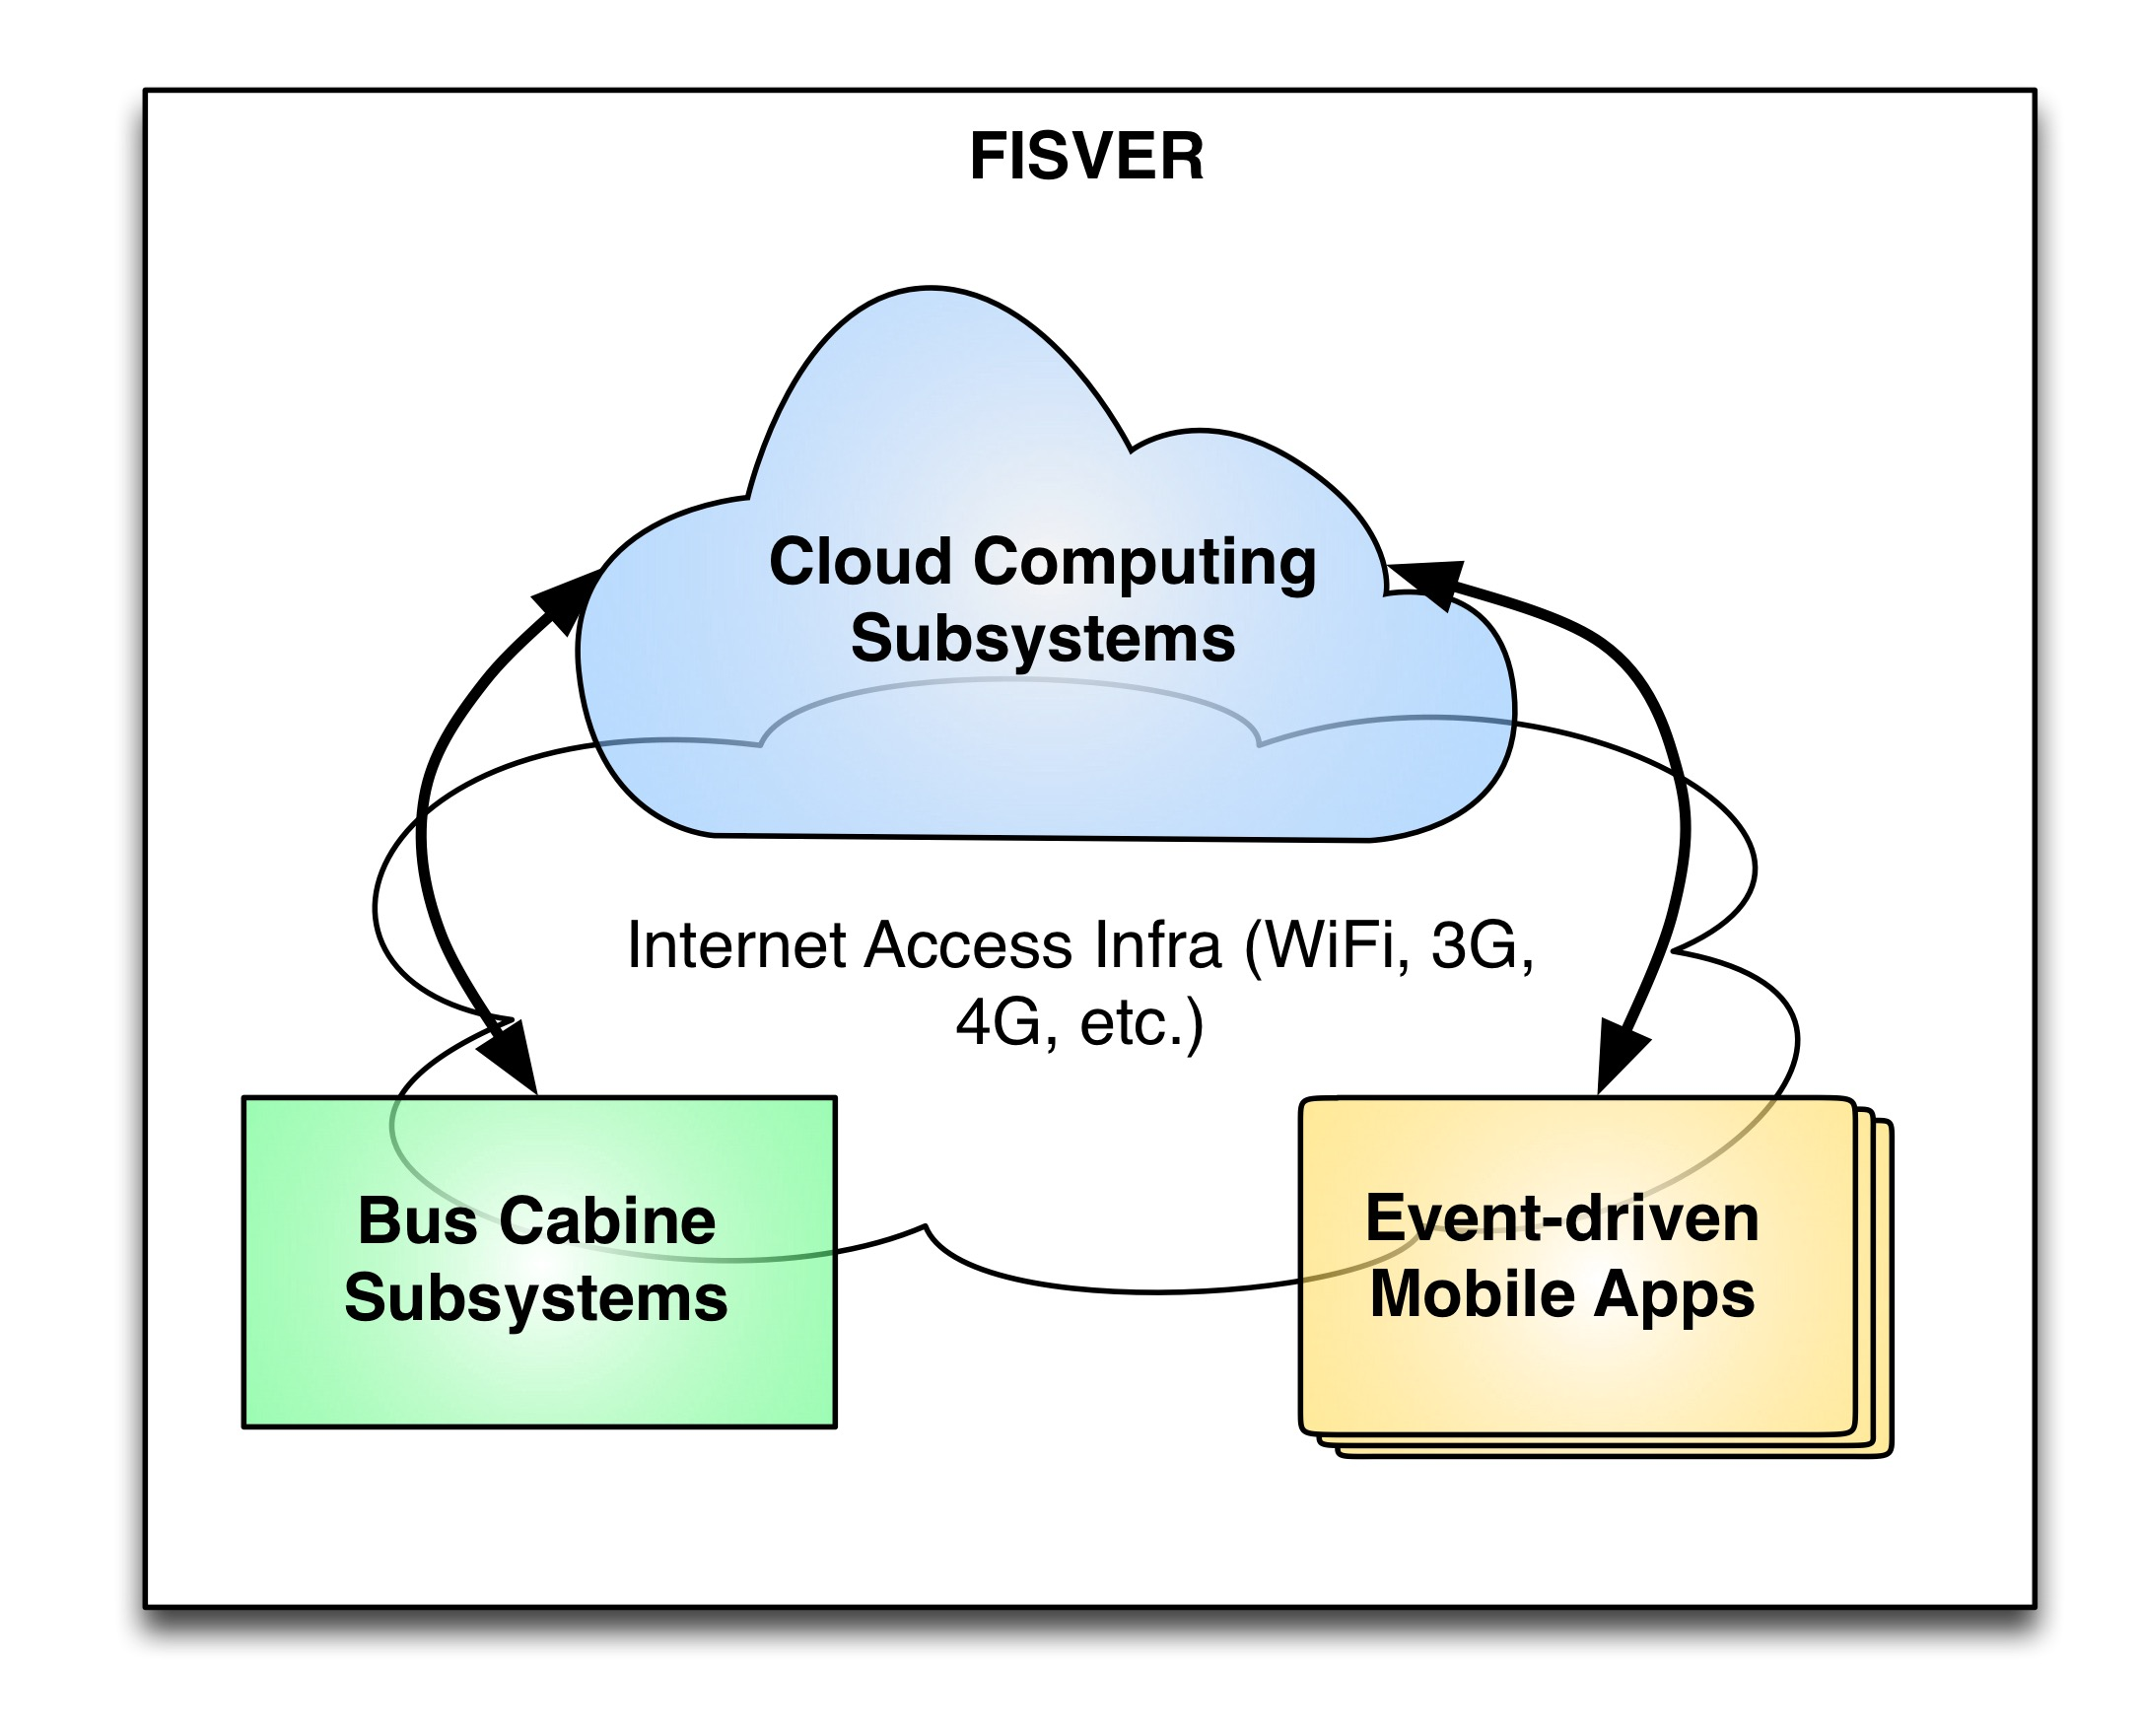
\includegraphics[scale=0.20]{Imagens/cap4_arch.png}
 	\caption{Main architecture for the proposed framework.}
 	\label{fig:arch}
\end{figure}

The FISVER key architecture is designed following a modular approach that features three interworking subsystems accessible via well-defined web-based external interfaces. In the FISVER modular architecture, each subsystem has clear divisions between subcomponents, which can be replaced/updated without affecting the rest of the system (in contrast to the integrated architecture). Each subsystem has their own architecture, featuring subcomponents that communicate each other via well-known internal interfaces. The key FISVER subsystems are described below:

\begin{itemize}

\item Bus Cabin Subsystems: This subsystem features a set of in-vehicle components responsible for: \textit{(i)} gathering sensory data in the bus cabin surrounding; \textit{(ii)} processing multimedia sensory data to afford identifying objects of potential security threats; \textit{(iii)} creating even crime level metadata; and \textit{(iv)} triggering the cloud infrastructure to provide crime level metadata for the targeted subsystems;

\item Cloud Infrastructure Subsystems: embeds a set of FISVER subsystems that exploit the powerful and scalable cloud computing infrastructure capabilities to afford large-scale storage, smart processing of sensory data and search of best suited crime assist units. The cloud services that can provisioned by the FISVER Cloud Infrastructure Subsystems are in the following: \textit{(i)} Templates as a Service, seeking to keep in-vehicle algorithms always up to date with new crime object patterns and/or new specific targets; \textit{(ii)} Event Classification as a Service, that exploits smart computing algorithms for classifying events in real-time based on the analysis in the image sent by the bus cabin subsystem; and \textit{(iii)} Crime Assist triggering as a Service, which addresses to find the best suited crime assist unit and further sending crime notifications to them for assistance;

\item Event-driven Mobile Apps: Runs on end user devices (e.g., smartphones/Tablets at crime assist units, third party safety centers, police authority control centers, etc.) deploying lightweight procedures. The event-driven mobile app is catheterized by mostly keeping in standby behavior until receiving crime notifications from the cloud Infrastructure subsystems, that are in turn presented to the users for appropriate assistance.
\end{itemize}

The FISVER approach is designed following the premise to run most complex smart computing procedures at the Bus Cabin and Cloud Infrastructure Subsystems. The FISVER approach foresees to achieve low networking overhead when compared to typical smart surveillance subsystems, since crime events may occur at lower periods of time (afforded by classifications of the cloud mechanisms). Moreover, typical smart surveillance subsystems keep constantly streaming multimedia data for remote processing, and beyond costly approach, such approach cannot guarantee QoE for assisting accurate detections. Details on each subsystem featuring the FISVER architecture are provided in the next.

\section{Bus Cabin Subsystems}

The Bus Cabin features a set of subsystems that are in charge to collect, process, and analyze multimedia data to detect crime threats in real-time. The Bus Cabin Subsystem key architecture design is depicted in Figure \ref{fig:buscabarq}.

\begin{figure}[htb!]
 	\centering
 	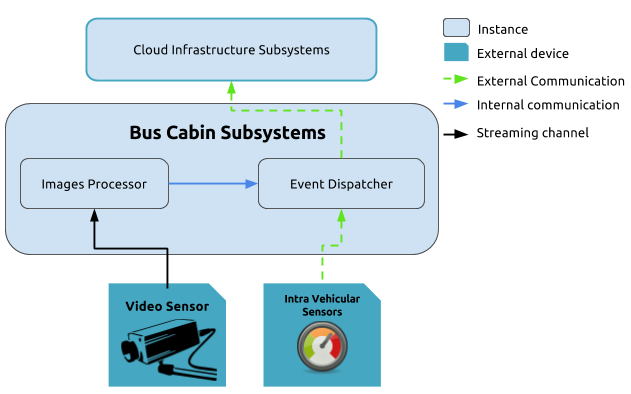
\includegraphics[scale=0.65]{Imagens/cap4_bus_cabin.png}
 	\caption{Bus Cabin Subsystem Architecture.}    
 	\label{fig:buscabarq}
\end{figure}
In next subsections \textbf{Images Processor} and \textbf{Event Dispatcher} are explained in details.
% * <augusto@dimap.ufrn.br> 2016-11-30T13:39:07.118Z:
%
% > FIGURA COM ARQUITETURA DO BUS-COMABIN MOSTRANDO Images Processor + Event Dispatcher + Intra-vehicular Sensors.
%
% Colocar figura da arquitetura do Bus Cabin aqui, e a seguir os subsistemas serão explicados. FAZER ISSO COM TOSO OS DEMAIS MODULOS QUE COMPÕE O FISVER........
%
% ^ <email@hugobarros.com.br> 2016-11-30T23:17:50.828Z:
%
% Feito
%
% ^.
\subsection{Images Processor}
% * <augusto@dimap.ufrn.br> 2016-11-30T13:19:33.415Z:
% 
% Ao que parece o modulo Bus Cabin é composto por Images Processor + Event Dispatcher+ mais algum? o tal Intra-vehicular Sensors? Vc deveria primeiramente apresentar a arquitetura geral do Bus Cabin Subsystem que mostre TODOS os subsistemas desse modulo e suas interfaces, e depois cada um deve ser descrito em suas devidas sub-sessões.
% 
% ^ <email@hugobarros.com.br> 2016-11-30T23:32:45.291Z:
%
% Feito acima, como descrito no comentário anterior. Os sensores são dispositivos externos.
%
% ^.
The Images Processor module is designed for downloading and updating the definitions in the algorithm configuration, for making new instances of image processing algorithms (one for each configuration), for comparing the input streaming in an attempt to find the specific target object, in which each algorithm was designed for, and lastly for storing definitions necessary for deploying algorithms. \ref{fig:buscab} depicts key features of the \textbf{Images Processor}.

\begin{figure}[htb!]
 	\centering
 	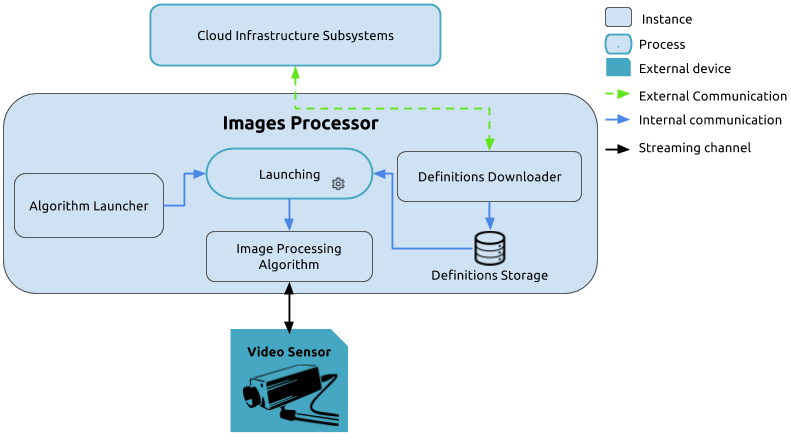
\includegraphics[scale=0.60]{Imagens/cap4_img_proc.png}
 	\caption{Features of Images Processor Subcomponent.}    
 	\label{fig:buscab}
\end{figure}

The key subcomponents featuring the Images Processor module are:
% * <augusto@dimap.ufrn.br> 2016-11-30T13:22:40.193Z:
% 
% > The key subcomponents featuring the Images Processor module are:
% > \begin{itemize}
% > \item \textbf{Definitions downloader:} at system bootstrap this component verifies if a new version or some new definition is available. In case of a new definition it will be downloaded and stored else if there is a new version of a definition it will be updated.
% > \item \textbf{Definitions Storage:} this component is responsible for storing all definitions and delivery them on query actions from algorithm instantiator.
% > \item \textbf{Algorithm instantiator:} after all definitions are downloaded and stored, the instantiator creates a new instance of each registered algorithm, passing as parameter the e specific configuration file containing parameters for one target object. All of them consuming the same streaming channel to collect and process images.
% ONDE ESTÁ O IMAGE PROCESSING ALGORITHM? ELE ESTÁ NA FIGURA APRESENTADO COMO UM SUBCOMPONENTE. E TEM AINDA O INSTATIATION (QUE PARECE NÃO SER UM SUBCOMPONENTE, MAS UMA ACÃO). SE FOR UMA AÇÃO NÃO DEVERIA CONSTAR NUMA FIGURA QUE APRESENTA UMA ARQUITETURA, POIS NÃO SE DESTINA A APRSENTAR AÇÕES, MAS COMPONENTES E INTERFACES. Ou não é uma figura de arquitetura mas um diagrama de fluxo?????? Defina isso e proceda como tal.
% 
% ^ <email@hugobarros.com.br> 2016-11-30T23:34:07.444Z:
%
% A figura é de fato da arquitetura, mas como a legenda mesmo mostra instantiation é um processo.
%
% ^.
\begin{itemize}

\item \textbf{Definitions downloader:} at system bootstrap this component verifies if a new version or some new definition is available. In case of a new definition it will be downloaded and stored else if there is a new version of a definition it will be updated.
\item \textbf{Definitions Storage:} this component is responsible for storing all definitions and delivery them on query actions from algorithm launcher.
\item \textbf{Algorithm launcher:} after all definitions are downloaded and stored, the launcher creates a new instance of each registered algorithm, passing as parameter the e specific configuration file containing parameters for one target object. All of them consuming the same streaming channel to collect and process images.
\end{itemize}
 
\textbf{Definitions Downloader} subcomponent, verifies if new version of definitions is available at \textbf{Cloud Infrastructure Subsystems}. It verifies too if a new object definition is registered. In this cases, definitions are downloaded and stored, for utilization at algorithms instantiation process. 
% * <augusto@dimap.ufrn.br> 2016-11-30T13:24:12.264Z:
%
% > invoked  at the system bootstrap
%
% A figura 4.2. apresenta que o Definitions Downloader é ativado no system bootstrapp???? NÃO, tem apenas módulos e setas.......aprenda rapaz.....
%
% ^ <email@hugobarros.com.br> 2016-11-30T23:35:16.713Z:
%
% corrigido
%
% ^.
Algorithm launcher in turn, creates an algorithm instance for monitoring images searching for a target object definition match. Images are acquired through a streaming channel, that are utilized by all algorithm instances. Details about Images Processor API subcomponents implementation with it methods and it parameters are shown in Table \ref{table algdep}.
% * <augusto@dimap.ufrn.br> 2016-11-07T22:34:17.937Z:
%
% > 1. ???
% > 2. ????
% > 3. ????
%
% Descrever em detalhes as funções disponíveis, a que se destinam cada uma, qual o resultado da implementação de cada, qual a sequência, etc etc etc.
%
% ^ <email@hugobarros.com.br> 2016-11-22T01:25:37.718Z:
% 
% feito em forma de tabela... faltando apenas uma forma de fazer merge nas celulas que possuem os nomes dos subcomponentes tornando a tabela mais organizada
% 
% ^.
\begin{center}
  \captionof{table}{Images Processor Subcomponent API}
  \label{table algdep} % for use in \ref{table1} if you want to refer to the table number
  \begin{tabular}{|c|c|c|c|c|c|}
  % etc.
  \end{tabular}
\end{center}
%\taburowcolors[2] 2{tableLineOne .. tableLineTwo}
%\tabulinesep = ^4mm_3mm
\tabulinesep=2.0mm
%\everyrow{\tabucline[.4mm  white]{}}

    \begin{tabu} to \textwidth {l >{\bfseries}X[r, 1.5] X[4,l,m]}
        \tableHeaderStyle
        
         & Method & Definition \\
       {\multirow{2}{*} {\rotatebox[origin=c]{90}{ \textbf{Defs. Downloader} }}} &verifyDef()&\small queries at cloud subcomponents if a new definition of of target object its available if yes download it and store it.\\
&verifyVers()&\small for each stored version of definitions this method verifies if a newer version is available, case true the local target object definition is updated.\\ \hline
\multirow{5}{*} {\rotatebox[origin=c]{90}{  \textbf{Definitions Storage} }}&\small getDefinition(String object)&\small returns latest version of a specific target object passed as parameter.\\
&\small getDefinition(String object, Integer version)&returns a passed as parameter version of a specific target object definition passed as parameter.\\
&\small addDefinition(String object)&\small creates a new version from a definition of target object passed as parameter. If no version exists for an object a new entry will be created for that object definition.\\
&\small purgeDefinition(String object)&\small Method utilized by \textbf{Definitions Downloader} in case of an old target object has been removed from system administrators .\\ \hline
{\rotatebox[origin=c]{90}{ \textbf{Algorithm Launcher} }}&init()&\small this method is called at finish of Definition Downloader tasks and is the last task of \textbf{Images Processor} bootstraping. It instantiates the image processing algorithms \\
\tabuphantomline
\end{tabu}
    
\hfill    
    
The sequence of interactions made between \textbf{Image Processor} subcomponents and their methods is shown in Figure \ref{fig:imgprocseq}. As described at the sequence diagram, \textbf{Definitions Downloader} triggers \textbf{Cloud Infrastructure} components following two main system events. 

\begin{figure}[htb!]
 	\centering
 	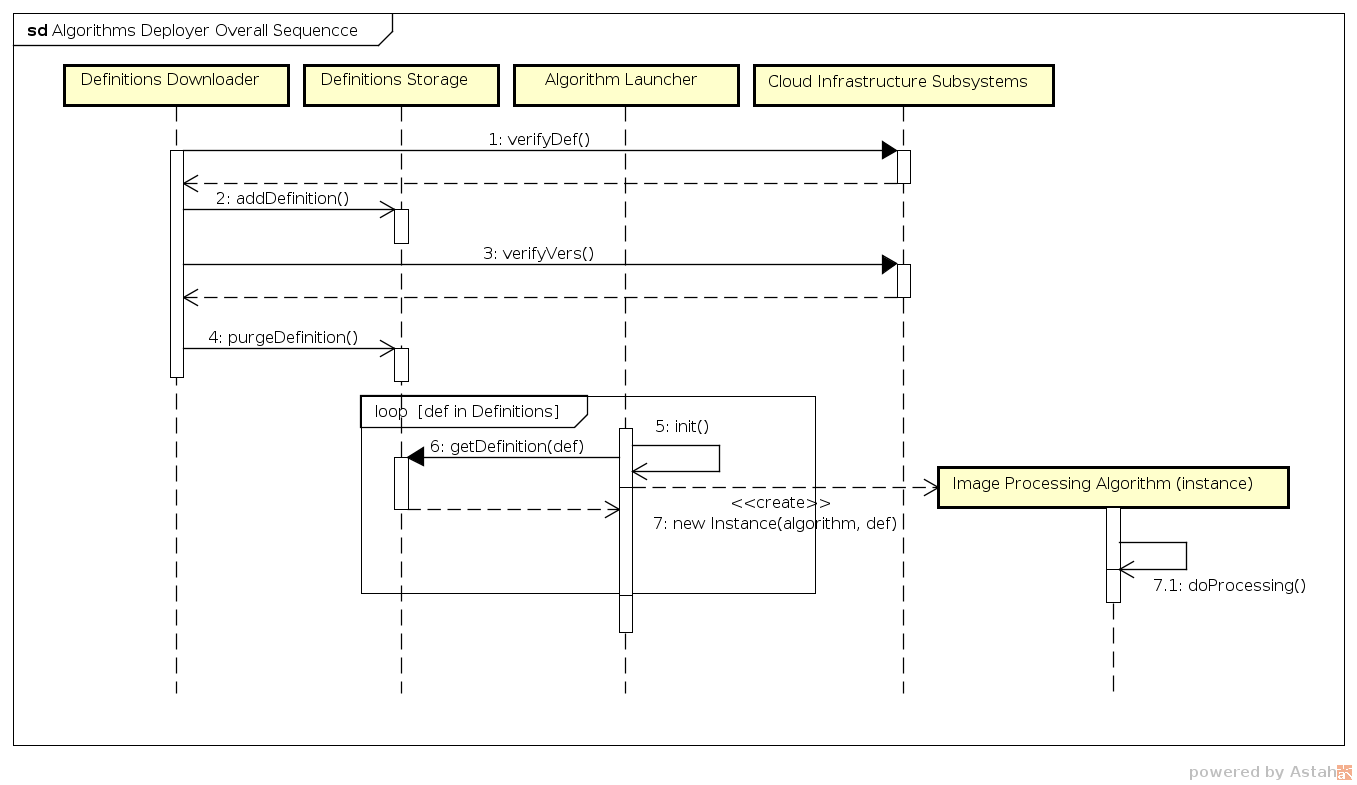
\includegraphics[scale=0.45]{Imagens/cap4_algseq.png}
 	\caption{Images Processor subcomponents overall sequence.}
 	\label{fig:imgprocseq}
\end{figure}

First for definitions updates, where existing objects definitions must be renewed. And second, for new target object definition registering, this occurs when new objects are registered at training phase, when system administrator collects several images of a target object for definitions extractions. 

% * <augusto@dimap.ufrn.br> 2016-11-23T18:21:57.279Z:
%
% > The sequence of interactions made between subcomponents and their methods described above is show in the sequence diagram below:
%
% Que sequencia? Descrito acima onde???? Não faça isso, use o nome da operação ou procedimento correspondente a sequência de interações que vc se refere.....não complica
%
% ^ <email@hugobarros.com.br> 2016-11-30T23:37:18.295Z:
%
% me referi ao diagrama de sequencia fig:imgprocseq
%
% ^.



% * <augusto@dimap.ufrn.br> 2016-11-30T12:25:30.013Z:
%
% > Instantiator
%
% Essa palavra "Instantiator" não existe no dicionário Inglês.......difícil viu
%
% ^ <email@hugobarros.com.br> 2016-11-30T23:58:09.935Z:
%
% Corrigido -> Algorithm launcher
%
% ^.

%\begin{figure}[htb]
% 	\centering
% 	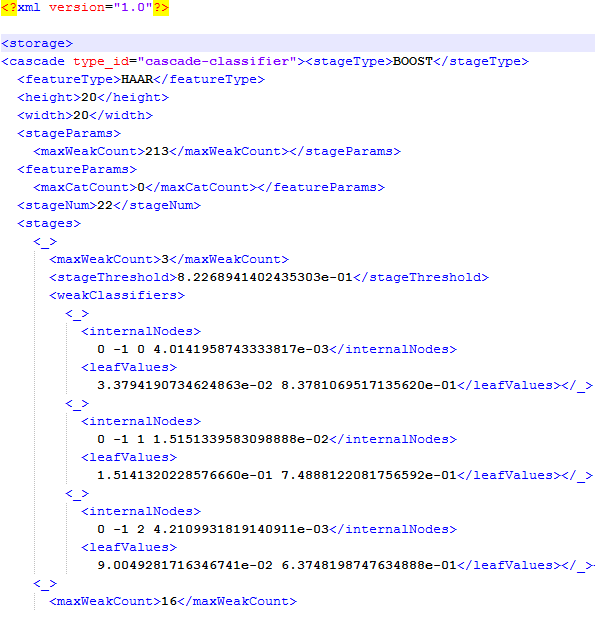
\includegraphics[scale=0.75]{Imagens/cap4_xml.png}
% 	\caption{Example of a configuration of an XML file.}
% 	\label{fig:xml}
%\end{figure}
% * <augusto@dimap.ufrn.br> 2016-11-07T22:30:03.855Z:
%
% > \begin{figure}[htb]
% >  	\centering
% >  	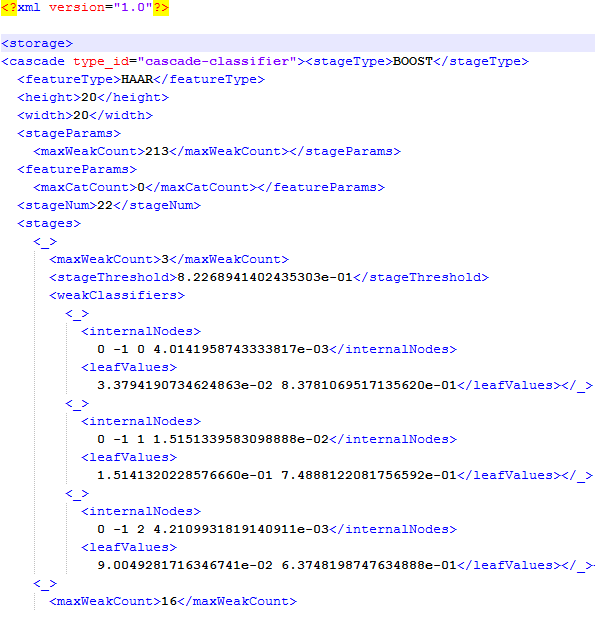
\includegraphics[scale=0.75]{Imagens/cap4_xml.png}
% >  	\caption{Example of a configuration of an XML file.}
% >  	\label{fig:xml}
% > \end{figure}
%
% Perceba que essa figura não aparece no item a que ela se destina apresentar, Bus Cabin Subsystem no caso, mas no texto ela vem no item de Cloud. Tem de haver uma maneira de controlar o posicionamento das figuras, porque simplesmente no texto INTEIRO isso ocorre, e só dá problema de entendimento e organização. 
%
% ^ <email@hugobarros.com.br> 2016-11-18T20:33:32.934Z:
%
% Resolvido... transformado em listing
%
% ^ <augusto@dimap.ufrn.br> 2016-11-30T12:23:32.085Z.


\subsection{Event Dispatcher Subcomponent}

The \textbf{Event Dispatcher} module is designed to aggregate information from both the \textbf{Images Processor} and the intra vehicular sensors(external devices). Once an event has been detected, this information is grouped in another XML type file which is prepared and sent to the for \textbf{Cloud Infrastructure Subsystems}. 
% * <augusto@dimap.ufrn.br> 2016-11-30T12:26:18.615Z:
% 
% "Images Processor and the Intra Vehicular Sensors"
% Cara, onde estão definidos esses subsistemas???? NENHUMA FIGURA das arquiteturas dos subsistemas constam estas entidades......Cara, tu não tem nenhum cuidado com isso, mostra tua total irresponsabilidade e desleixo com o trabalho.
% 
% ^ <email@hugobarros.com.br> 2016-11-30T23:59:17.488Z:
%
% external devices... corrigido
%
% ^.

\begin{figure}[htb!]
 	\centering
 	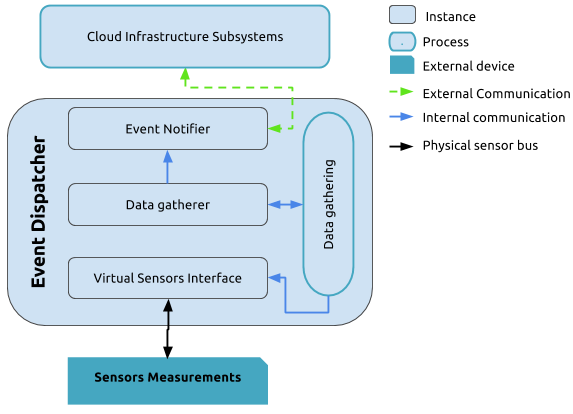
\includegraphics[scale=0.70]{Imagens/cap4_evtdspt.png}
 	\caption{Features of Event Dispatcher Subcomponent.}    
 	\label{fig:evtdspt}
\end{figure}

The subcomponent supported at the Event Dispatcher are:

\begin{enumerate}

\item \textbf{Event Notifier:} this subcomponent is responsible for collect data extracted from array of sensors an send it to \textbf{Cloud Infrastructure Subsystems}. As example: GPS location of bus at event moment, vehicle speed and fire sensor, but there are no limit for data extracted from any sensor available and registered for sensing.
\item \textbf{Data gatherer:} makes an edge from \textbf{Event Notifier} and sensors. The data is collected from sensor through a interface which implements an abstract layer for real sensor information. In this component data can be normalized, and converted when necessary.
\item \textbf{Virtual Sensors Interface:} this interface implements a virtual layer for data sensing. The sensor data can be collect from different sources each one with an specific protocol. So this interface realizes sensor data collection between different protocols.

\end{enumerate}

As said previously, \textbf{Event Dispatcher} component is called when an \textit{algorithm instance} matches a given image with a target object configuration. When this occurs, \textbf{Event Notifier} is called by an \textit{algorithm instance} and through \textbf{Virtual Sensors Interface} it collects all available sensory data to compose event message(aggregated in a XML file as exemplified in Listing \ref{event_file}).

\textbf{Data Gatherer} subcomponent is utilized at this step, for provide raw sensor data conversions(when necessary). For each registered sensor it can, do it based on the sensor interface implementation. It also verifies when sensor data is availabe or not for data collecting. 

For many causes, a sensor become unavailable and the process of collecting this sensor data may cause some delays. In this case \textbf{Data Gatherer} make array of sensors availability control for avoiding this kind of issue.

The \textbf{Event Notifier} that works at top of \textbf{Event Dispatcher} stack. It receive an \textit{algorithm instance} call, and after all process done by the \textbf{Data Gatherer} it prepares an event XML file, that will be sent to \textbf{Cloud Infrastructure Subsystems} in which receives this events through a web service.


In Listing \ref{event_file}, is shown an example of a generated XML file to report an event occurrence by the \textbf{Event Notifier}:

\begin{changemargin}{0.5cm}{0.5cm} 
\begin{center}
\begin{lstlisting}[caption={Example of an event XML file.},label={event_file},language=XML]
<?xml version="1.0"?>
<event>
    <!-- Potential threat event instance --!>
  <bus id="9999">
    <location>
      <lat>5.840592</lat>
      <long>-35.1999164</long>
    <location>
    <company id="45">
      <name>Example Company</name>
      <line>45</line>
  </bus>
  <avg_speed>40</avg_speed>
  <fire>false</fire>
  <algorithm  id="1001" name="cascade_classifier">
    <image_res>640_480</image_res>
    <detectime></detectime>
  </algorithm>
  <image_cut>
    R0lGODlhPQBEAPeoAJosM//AwO/AwHVYZ/z595kzAP/s7P+goOXMv8+
  </image_cut>  
</event>  
\end{lstlisting}
\end{center}
\end{changemargin}

In making it possible to establish communication with the \textbf{Cloud Infrastructure Subsystems} web service, the \textbf{Event Dispatcher} was designed to send grouped information (sensors, detectors and classifiers) in one compressed XML file(as in example shown above). Sensor Measurements, are external sensing devices, which are acessed through a textit{class} that implements \textbf{Virtual Sensors Interface}. This data is collected through an ODB2\footnote[19]{ODB2 connection implemented by \textbf{Virtual Sensors Interface}. http://www.obdii.com/. \textit{Accessed on December 10th, 2015.}} bus that can acquire data about the factory sensors e.g. speed, engine details, temperature etc.

In table \ref{table evt} a detailed description is shown for each method in \textbf{Event Dispatcher} subcomponent:

\begin{center}
  \captionof{table}{Event Dispatcher API}
  \label{table evt} % for use in \ref{table1} if you want to refer to the table number
  \begin{tabular}{|c|c|c|c|c|c|}
  % etc.
  \end{tabular}
\end{center}
%\taburowcolors[2] 2{tableLineOne .. tableLineTwo}
%\tabulinesep = ^4mm_3mm
\tabulinesep=2.0mm
%\everyrow{\tabucline[.4mm  white]{}}

    \begin{tabu} to \textwidth {>{\bfseries}l >{\bfseries}X[r, 1.5] X[4,l,m]}
        \tableHeaderStyle
        
         & Method & Definition \\
        {\multirow{2}{*} {\rotatebox[origin=c]{90}{Event Notifier}}}&\small prepareEvent(AlgEvent algevt)&\small receives an object with all details related to \textbf{Images Processor} processing. With this signaling, \textbf{Event Dispatcher} will make operations necessary to aggregate all data to report an event.\\
&sendEventNotification()&\small prepares, export and send a package within XML file format to \textbf{Cloud Infrastructure Subsystems}, this package contains all information about an event.\\ \hline
{\multirow{2}{*} {\rotatebox[origin=c]{90}{Data gatherer}}}&\small isAvailable(Integer sensorID)&\small verifies if a sensor is turned on and at normally functioning. Returns \textit{true} in positive case and \textit{false} in other cases.\\
&getAvailableData()&\small query all available sensor information normalizing and converting them when necessary.\\ \hline
{\multirow{2}{*} {\rotatebox[origin=c]{90}{Virtual Sensor Interface}}}&\small registerSensor(Integer sensorID, Class <class>)&\small creates a virtual sensor with an id. The implementation of real data the will be extracted from this sensor are made by a java class passed as parameter.\\
&getData(Integer sensorID)&\small instantiates the class registered for the specific sensor passed as parameter, and realizes all operations implemented for real data recovery.\\
\end{tabu}

\hfill

\textbf{Event Notifier} receives a call from \textbf{Images Processor}, which pass as parameter an object containing details about the target object matching, including image crop of acquired image containing the matched object. 
\textbf{Data Gatherer} in turn is called, which will look for all available sensors. Once available sensors are enumerated, all available data is collected using \textit{getAvailableData()} method. In this step a conversions and data treatment can be done depending on type of sensor and desired data.

\begin{figure}[htb!]
 	\centering
 	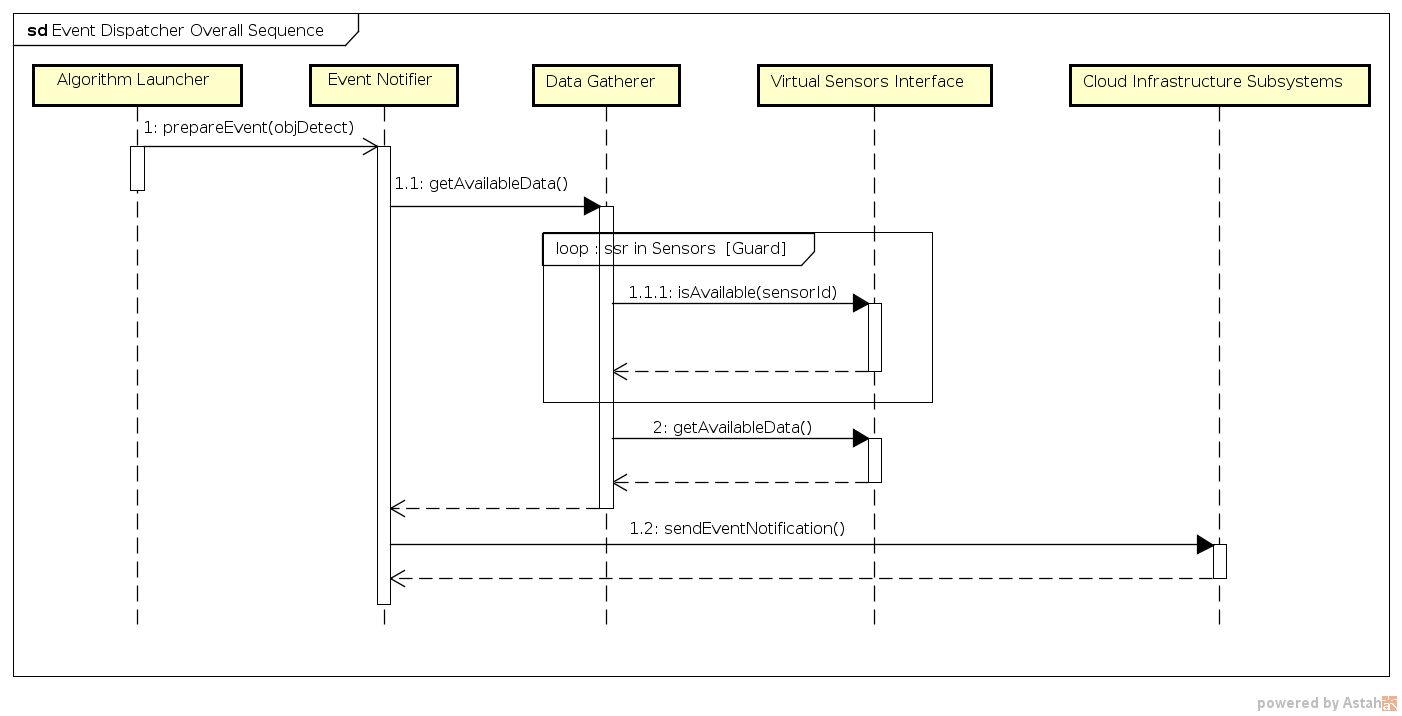
\includegraphics[scale=0.45]{Imagens/cap4_evtdsp.png}
 	\caption{Event Dispatcher subcomponent overall sequence.}
 	\label{fig:evtseq}
\end{figure}

\textbf{Virtual Sensors Interface} serves raw sensor data information to \textbf{Data Gatherer} subcomponent. It has functions for registering sensor and collect sensor raw data. In registering phase, done through \textit{registerSensor()} method, a \textit{class} that implements all details of raw data acquirement is passed as parameter. This classes implements \textbf{Virtual Sensor Interface} and are also responsible to implement details for sensors measurements acquirement, as example ODB2 communication for factory vehicle sensors measurements. The access of this sensors data can be made through serial port or Bluetooth \footnote[20]{Bluetooth Technology. https://www.bluetooth.com/. \textit{Accessed on December 10th, 2015.}} and this \textit{class} will be responsible for treating this assessment. After all this steps, \textbf{Event Notifier} send full event information to \textbf{Cloud Infrastructure Subsystems} through the method \textit{sendEventNotification()}. This communication is done through web service, and the information received will be treated by subcomponents that will be described at next subsection.


\section{Cloud Infrastructure Subsystems}

The Cloud Infrastructure Subsystem are in charge for deploying smart procedures to classify the received crime threats indications, and if confirmed, best suited crime assist unit(s) is(are) then searched and triggered to deal with the crime at the location. The FISVER approach relies on the possibility to benefit the overall system with the large-scale performance capabilities (i.e., processing, storage, and other key resources) that are commonly provisioned by the cloud-capable infrastructures. In Figure \ref{fig:cloud_infra}, there is a description of key component designs that will be deployed in a specific cloud provider to support both the Bus Cabin components and Event-driven Mobile Application.

\begin{figure}[htb!]
 	\centering
 	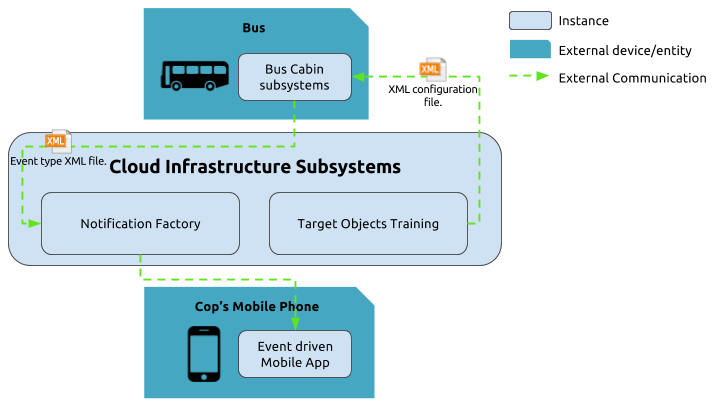
\includegraphics[scale=0.65]{Imagens/cap4_cloud_infra.png}
 	\caption{Cloud Infrastructure Subsystems Architecture.}
 	\label{fig:cloud_infra}
\end{figure}

The intercommunication between the Bus Cabin and the Cloud Infrastructure subsystems is carried out through SOAP\footnote[21]{SOAP W3C Specification. https://www.w3.org/TR/soap/. \textit{Accessed on December 10th, 2015.}} Web Service specification. Layers interaction are illustrated in the Figure \ref{fig:soap} below:

\begin{figure}[htb!]
  \centering
  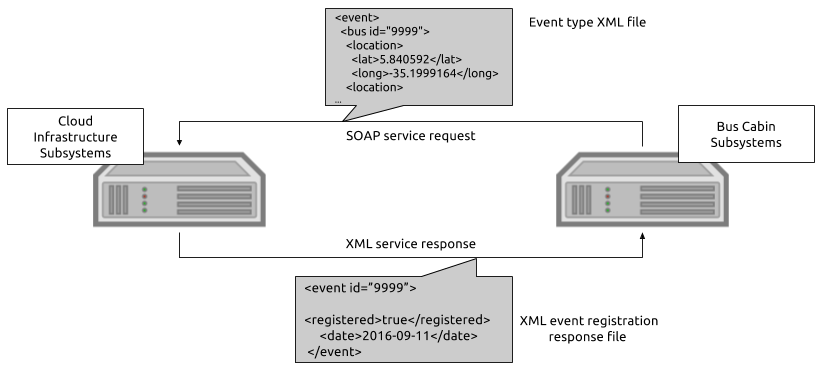
\includegraphics[scale=0.50]{Imagens/cap4_soap_arq.png}
  \caption{SOAP communication overview between FISVER layers.}
  \label{fig:soap}
\end{figure}

Figure \ref{fig:soap}, shows an example of message swapping between \textbf{Bus Cabin Subsystems} and \textbf{Cloud Infrastructure Subsystems} at the moment of a crime threat detection. In this example an Event notification is sent as a SOAP service request. As response \textbf{Bus Cabin Subsystems} receives information related to event registration (as example \textit{id} and \textit{date}). At next subsections, details about \textbf{Target Object Training} and \textbf{Notification Factory} subcomponents are given.

%https://www.w3.org/2000/xp/Group/
% * <augusto@dimap.ufrn.br> 2016-11-07T22:39:21.758Z:
%
% > The intercommunication between the Bus Cabin and the Cloud Infrastructure subsystems is carried out through...
%
% webservice???? Como se comunicam? Nao basta dizer que um manda mensagem ao outro, COMO ISSO É FEITO? Que protocolo? Quais mensagens são definidas na Accebility interface???? Que funções estão disponíveis????? Po, tu não uma planilha no excel pra isso, são aplicações que funcionam em rede.......
%
% ^ <email@hugobarros.com.br> 2016-12-01T04:55:48.664Z:
%
% in progress
%
% ^.

\subsection{Target Object Training}
% * <augusto@dimap.ufrn.br> 2016-11-07T22:50:47.924Z:
%
% > Target Object Training}
%
% Descreva em subitens todos os subcomponentes de cada subsistema, com todas as informações necessárias e as devidas especificações e elementos que possam descrever isso
%
% ^ <email@hugobarros.com.br> 2016-12-01T04:56:10.680Z:
%
% feito na versão anterior
%
% ^.
\begin{figure}[htb!]
  \centering
  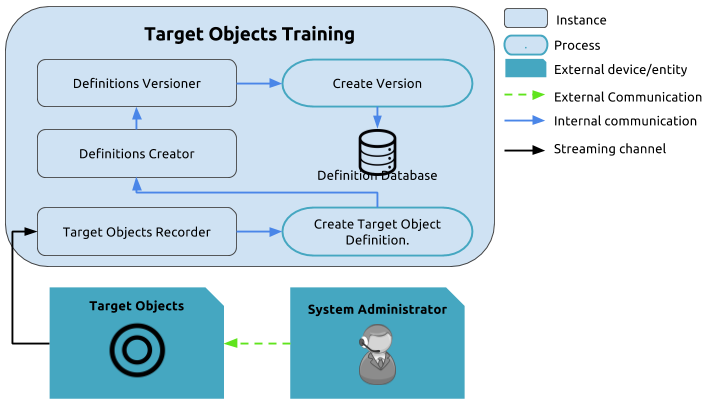
\includegraphics[scale=0.65]{Imagens/cap4_objtraining.png}
  \caption{Object Training Subcomponent.}
  \label{fig:objt}
\end{figure}
Since there is a wide range of target objects, the Target Object Training Module makes it possible to add new objects for purposes of recognition. These can only be accessed by the police authorities (i.e. a security analyst), who can insert, update or delete target object \textit{definitions}. The main task of \textbf{Target Object Training} is create, update and store target object \textit{ definitions} for updating all the \textbf{Bus Cabin} instances in which \textbf{Images Processor} subcomponent uses them through \textbf{Algorithm Launcher} as parameter for a target object matching. In Figure \ref{fig:objt} details about \textbf{Target Objects Training} subcomponent are depicted. The proposed approach creates \textit{definitions} for target object management. These definitions are based on the color and shape of the target objects. Data extracted from \textbf{Definitions Creator} subcomponent, creates a file containing relevant information such as the color of the gradient and shape of the objects. Definition extraction process is done through OpenCV\footnote[22]{Open Source Computer Vision Library. 
http://docs.opencv.org/2.4/index.html \textit{Accessed on December 10th, 2015.}} library. \textbf{Target Objects} are dangerous objects utilized in crime threats. They are selected by the system administrator before training phase for any causes. One cause is to improve \textbf{Bus Cabin} dispatched events(avoid false alarms) another cause is to add new set of \textbf{Target Objects} for \textbf{Images Processor} subcomponent matching(at \textbf{Bus Cabin Subsystems}).
For definitions creation is necessary a set of samples. There are two types of samples: negative and positive. Negative samples correspond to non-object images. Positive samples correspond to images with detected objects. Set of negative samples must be prepared manually, whereas set of positive samples is created using OpenCV API. \textbf{Target Objects Recorder} subcomponent is reponsible for acquire positives images(through a streaming channel) and store them temporally. \textbf{Definitions Creator} gets union of positives samples and generates \textit{definitions} based of features extracted from positives samples. The Listing \ref{config_file} shows an example of a \textit{definition} file created at this step: 
%Base64\footnote[18]{Online Decode. http://www.onlinedecode.com/about-base64/. \textit{Accessed on December 10th, 2015.}} image datasets for training when necessary. 

\begin{changemargin}{1.5cm}{1.5cm} 
\begin{center}
\begin{lstlisting}[caption={Example of a target object definition file.},label={config_file},language=XML]
<?xml. version="1.0"?> 
<!-- configuration file for a target object detection --!>
<storage> 
 <cascade type_id="cascade-classifier">
  <stageType>BOOST</stageType> 
   <featureType>HAAR</featureType> 
    <height>20</height> 
    <width>20</width> 
   <stageParams> <maxWeakCount>213</maxWeakCount> </stageParams> 
   <featureParams>  <maxCatCount>0</maxCatCount> </featureParams> 
   <stageNum>22</stageNum> 
   <stages> 
    <maxWeakCount>3</maxWeakCount> 
	<stageThreshold>8.2268941402435303e-01</stageihreshold>
	<weakClassifiers> 
	 <internalNodes> O -1 0 4.0141958743333817e-03</internalNodes>
	 <leafValues> 3.3794190734624863e-02 8.3781069517135620e-01
     </leafValues>
    </weakClassifiers>
    </stages>
</storage> 
\end{lstlisting}
\end{center}
\end{changemargin}

This XML file is generated during the training phase with extraction of features by positives target objects images. This features will be utilized by the \textbf{Algorithm Launcher} as a parameter in algorithm launching process at \textbf{Bus Cabin Subsystems}. Table \ref{table to} show detailed description about each \textbf{Target Objects Training} subcomponent methods:
\begin{center}
  \captionof{table}{Target Objects Training API}
  \label{table to} % for use in \ref{table1} if you want to refer to the table number
  \begin{tabular}{|c|c|c|c|c|c|}
  % etc.
  \end{tabular}
\end{center}
%\taburowcolors[2] 2{tableLineOne .. tableLineTwo}
%\tabulinesep = ^4mm_3mm
\tabulinesep=2.0mm
%\everyrow{\tabucline[.4mm  white]{}}

    \begin{tabu} to \textwidth {>{\bfseries}l >{\bfseries}X[r, 1.5] X[4,l,m]}
        \tableHeaderStyle
%% forma de fazer com multirow http://tex.stackexchange.com/questions/111249/multirows-multicolums-and-vertical-centring-in-the-tabu-environment        
         & Method & Definition  \\
        {\multirow{2}{*} {\rotatebox[origin=c]{90}{\small Target Objects Recorder}}}&trainNewObJ(Image[] imgarray)&{receives an image array from the new object to be recorded and extract it caracteristics, that will used for create definition.}\\
        &trainExistingObj(Image[] imgarray, boolean merge)&{update an object definition, based on new image array passed as parameter, with option to merge current definition with new or overwrite all definitions with new images, signaled by boolean parameter merge.}\\ \hline
{\multirow{2}{*} {\rotatebox[origin=c]{90}{Defs. Creator}}}&consolidateTraining()&{realizes validation in definitions created by \textbf{Target Object Definition processs} and generates XML definition file that will be passed for \textbf{Definitions Versioner}}.\\
&mergeDefinitions(Integer defIDFrom, Integer defIDTo)&{merges passed as id parameter the definitions, this method is called by \textbf{Target Objects Recorder} when the update process of an existing object was called passing the merge parameter with \textit{true} value.}\\ \hline
\rotatebox[origin=c]{90}{Defs. Versioner}&defineVersion(Integer objectID, Definition def)&{based on a registered object this method defines how different a previous version is from the newer that will be addded to \textbf{Definitions Database}, gived a new version number, this objects will be stored at \textbf{Defs Database}.}\\ \hline
{\multirow{2}{*} {\rotatebox[origin=c]{90}{Definitions Database}}}&storeDef(Integer objectID, Definition def, Version ver)&{ stores a passed as parameter definition, related to an object passed as parameter too.}\\
&getCurrentDefs()&{ returns all active \textit{Target Ojbects Definitions}. This  method is used by the all instances of \textbf{Images Processor} in it bootstraping to make objects updates.}\\

\end{tabu}
\hfill

When \textit{definition} creation process is completed, \textbf{Definitions Versioner} is called to verify if already exists a trained target object definition, if doesn't exists, a new entry is created for that objects as primary version. Case already exists, definition will receive a new version that will be registered for that target object and stored at \textbf{Definitions Database}. 
At the finish of \textit{definition} creation, a file containing target objects feature extraction values is generated. This values will be used by all \textbf{Bus Cabin Subsystems} instances when updated through \textbf{Definitions Downloader} subcomponent as detailed in previous section. After checking any changes in the \textbf{Definitions Database} the \textbf{Definitions Versioner} module generates a new target object definition version. The \textbf{Definitions Database} handles the storage of all the textit{definition} versions and their creation of data, as well as noting the users who created them and their observations.

% * <augusto@dimap.ufrn.br> 2016-08-22T21:56:12.822Z:
%
% Essa figura precisa ser explicada passo a passo, comentando a sequência realizada no diagrama. Eu acho que a especificação neste capítulo é mt insuficiente, parece descrever uma coisa muito simples (6 páginas). Use e abuse de diagramas, como diagramas de estado, isso enriquece o capítulo principal da dissertação, que descreve a proposta em "detalhes"....mas carede dos tais detalhes.
%
% ^ <augusto@dimap.ufrn.br> 2016-10-16T23:59:27.499Z:
%
% Isso aqui não foi feito no documento, o que falta? Explica o diagrama de sequência....
%
% ^.

% * <email@hugobarros.com.br> 2016-10-05T19:55:20.110Z:
%
% https://www.websequencediagrams.com/
%
% ^ <email@hugobarros.com.br> 2016-11-05T21:30:22.494Z.


%The \textit{Data Gathering} module acts as an interface between the Bus Cabin and Cloud Components, and checks each new Alert package to find out if the quality of the information meets the requirements necessary before the security analysts can be notified . If the \textit{Data Gathering} approves the quality of the %\textit{contextualAlertPackage}, it is sent to the \textit{Publish Manager} who is called on to publish the alert to the mobile applications.

\subsection{Notification Factory}

\textbf{Notification Factory} subcomponent, is responsible for receive \textit{event notifications}, sent by all \textbf{Bus Cabin Subsystems} instances. In Figure \ref{fig:notfact} details about \textbf{Notification Factory} subcomponent architecture are shown:

%The Data Gathering module receives all the information sensed by the bus cabin system; and this information can be further made use of by deploying the applications in the proposed cloud services. The purpose of the Publish Manager is to catalog communication information and send it to an interested context-driven application whenever an event occurs. 

%In Figure \ref{fig:workflow}, there is a generic workflow which explains more clearly the updated templates, object detection, context generation and publishing process.
%At least one object template registered at Templates Database is required to initiate the recognition procedure. Once the Templates Database is populated, the Object Detector can retrieve templates and start the detection process. If the similarity measure reaches a threshold (which is established by security analysts as a parameter), the Object Detector will notify the Event Manager about the region that is matched with a target object template. Event Manager, in turn collects the sensor information (GPS, Velocity, etc.) and creates a contextual Alert Package by sending it to Data Gatherer. 

%\begin{figure}[htb!]
% 	\centering
% 	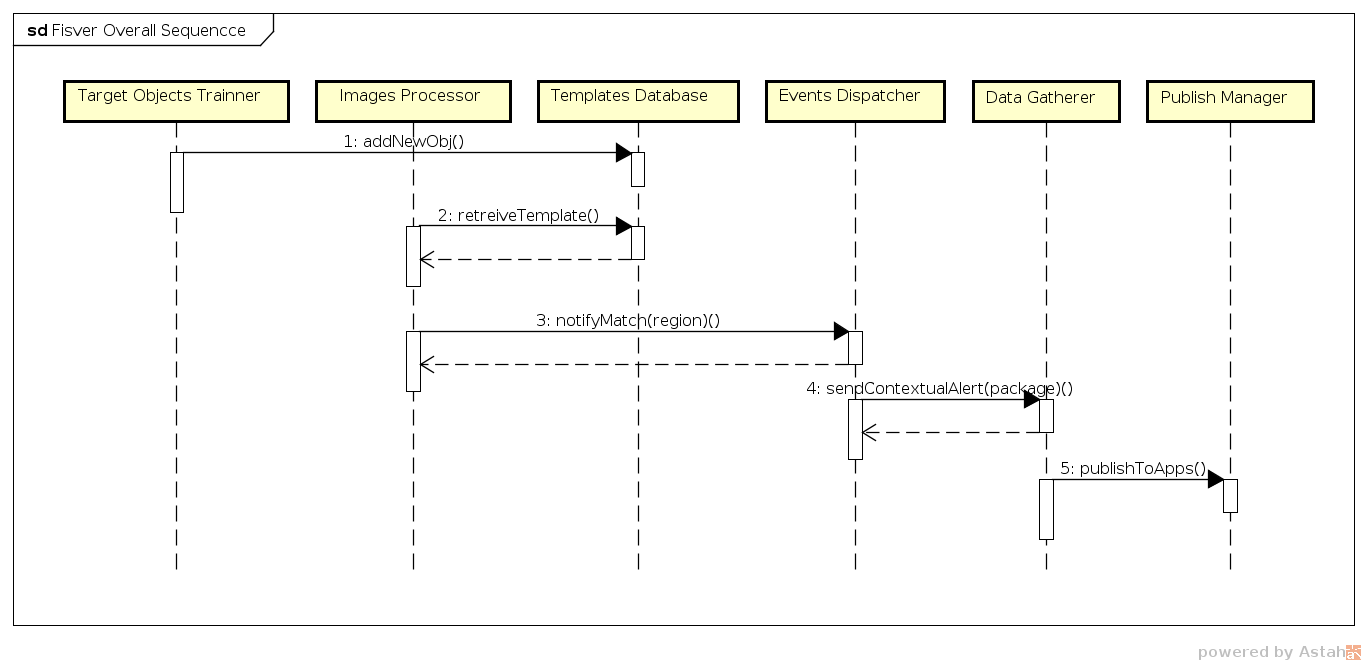
\includegraphics[scale=0.45]{Imagens/cap4_fisver_over_seq.png}
% 	\caption{Fisver cloud components overall sequence.}
% 	\label{fig:workflow}
%\end{figure}



%At least one object template registered at \textit{Templates Database} is required to initiate the recognition procedure. Once the \textit{Templates Database} is populated, the \textit{Object Detector} %can retrieve templates and start the detection process. If the similarity measure reaches a threshold (which is established by security analysts as a parameter), the \textit{Object Detector} will notify %the \textit{Event Manager} about the region that is matched with a target object template. \textit{Event Manager}, in turn collects the sensor information (GPS, Velocity, etc.) and creates an Alert %Package by sending it to \textit{Data Gathering}. 

\begin{figure}[htb]
 	\centering
 	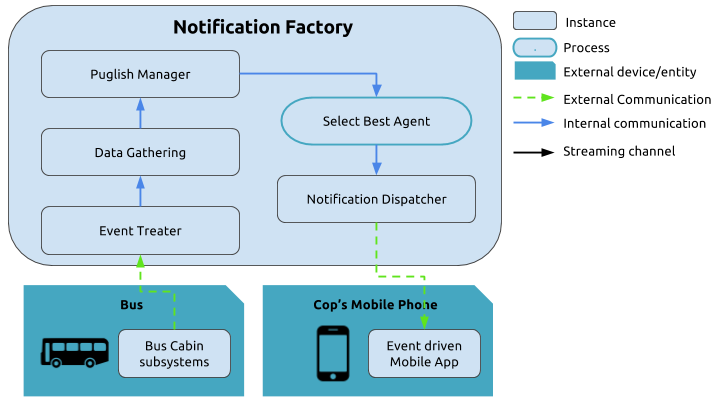
\includegraphics[scale=0.65]{Imagens/cap4_notffact.png}
 	\caption{Notification Factory Subcomponent.}
 	\label{fig:notfact}
\end{figure}
Once a threat \textit{event} is dipatched from \textbf{Bus Cabin Subsystems}, the \textbf{Event Treater} subcomponent is able to make validations about that received event. In order guarantee \textbf{Cloud Subsystems} service continuity, \textbf{Event Treater} works with a processing queue in which, incoming \textit{events} are received and queued for a validation process in order to discard wrong \textit{events} messages. This validation is made over \textbf{Bus Cabin Subsystem} entry if it has a valid registered \textit{id}. In \textit{event} validation process, \textit{sensors measurements} are also validated to avoid triggering all \textbf{FiSVER} stack to alert about a wrongly sent event, as example an \textit{event} in which sensed \textit{GPS location} reports an event at a jungle, where is impossible to ride by bus.
In table \ref{table notf}, we show each method specification:

\begin{center}
  \captionof{table}{Notification Factory API}
  \label{table notf} % for use in \ref{table1} if you want to refer to the table number
  \begin{tabular}{|c|c|c|c|c|c|}
  % etc.
  \end{tabular}
\end{center}
\tabulinesep=2.0mm
    \begin{tabu} to \textwidth {>{\bfseries}l >{\bfseries}X[r, 1.5] X[4,l,m]}
        \tableHeaderStyle
        
         & Method & Definition  \\
    	Event Treater&receiveEvent()&receives an \textit{event notification} and realizes all validations necessary to forward event to next subcomponents.\\
        Data Gathering&unpackEvent()&makes received event unpacking and register event details for analysis. \\
Publish Manager& publishNotification() &Selects the best(nearest) agent to deliver the notification.\\
Notification Dispatcher&sendNotification()&Prepares notification and send it to selected agent.\\

\end{tabu}



The \textit{unpackEvent()} method, calls all \textit{Classes} with \textbf{Data Gathering} interface implementation. The \textbf{FISVER} approach, turns possible addition of new actions at \textbf{Cloud Infrastructure} layer. This actions are implemented by classes with \textbf{Data Gathering} abstract methods implementations, containing all details for registering events and making decisions, as event delivering or not.

%\begin{figure}[htb!]
% 	\centering
% 	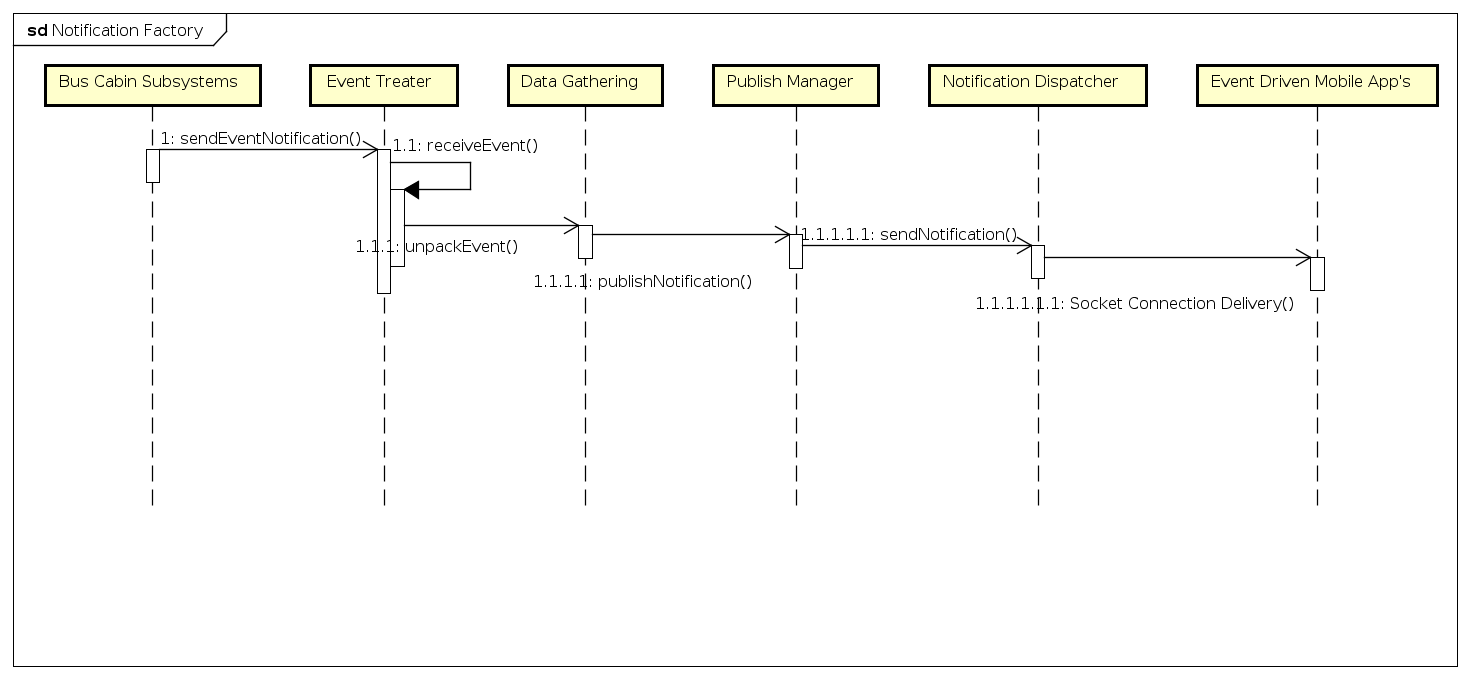
\includegraphics[scale=0.45]{Imagens/cap4_notifackseq.png}
% 	\caption{Notification Factory operation sequence.}
% 	\label{fig:seqnotfac}
%\end{figure}



\section{Event-driven Mobile Applications}
% * <augusto@dimap.ufrn.br> 2016-11-07T22:52:09.386Z:
%
% > Event-driven Mobile Applications}
%
% Especifique a aplicação, diagrama de estado dela, como é ativada (webservice????), que metadados ela recebe, benefícios do event-driven, ETC ETC ETC ETC. Vc acha que e parágrafos minúsculos e esta figura descrevem isso?
%
% ^.
Currently, proven cloud services can facilitate the development of any application, whether it be mobile or desktop. In view of the benefits expected from the components set out in the proposed framework cloud model, a wide range of applications for smart public safety can be anticipated. In light of this, we designed an Event-driven mobile application use case as a \textit{"proof-of-concept"} as an easy way to integrate and deploy applications through the use of FISVER. In Figure \ref{fig:app} an event alert was sent to a police agent smartphone:


\begin{figure}[htb]
 	\centering
 	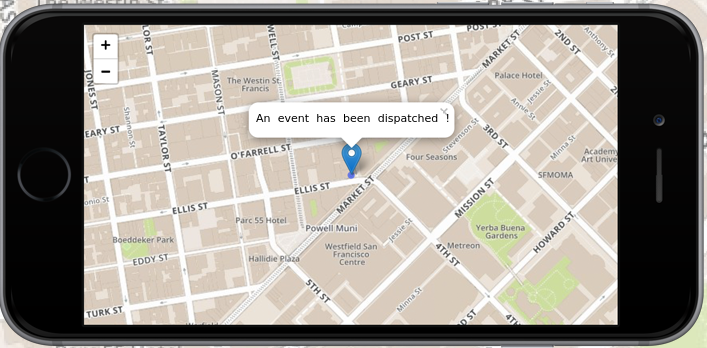
\includegraphics[scale=0.50]{Imagens/cap4_app.png}
 	\caption{Prototype of a Mobile application.}
 	\label{fig:app}
\end{figure}


The information extracted from several instances and grouped in the proposed framework can benefit governments by offering them new opportunities to plan and maintain a lot of applications. One example of an application considered in this scenario was employed in the police car, probably in a tablet or in the cop's smartphone that contains the GPS location. 

With the aid of this information the nearest police car can be warned by receiving an alert about a crime event occurring in a bus, together with the bus directions (future location of the bus in a street or venue) and thus make any intervention easier.
% * <augusto@dimap.ufrn.br> 2016-08-22T21:59:21.740Z:
%
% Acho que vc poderia fechar este capítulo com a descrição de um Use Case,  para concretamente exemplificar o uso da ferramenta, e tbm somar mais ao capítulo que está mt pobre enquanto especificação....
%
% ^.
\section{Conclusion}
% * <augusto@dimap.ufrn.br> 2016-08-22T21:57:57.608Z:
%
% Overview?????? Não né, o capítulo dis "Detailed descriptio.....", e não overview. Vc precisa descrever em detalhes, muitos detalhes.......não reflete isso este caoítulo....
%
% ^.
In this chapter, there was an overview of the FISVER architecture. Details about each \textbf{FISVER} \textit{subcomponent} were described as well as the interaction all of them. The next chapter will include an evaluation of the scenarios and results.
	
	% Capitulo 5: Quinto capítulo (arquivo Includes/Capitulo5.tex)
	% Capítulo 5 
\chapter{Evaluation}

This chapter addresses to check the suitability of the FISVER approach in provisioning cloud-enabled Smart Surveillance based transportation-safety systems. In general, the success of smart surveillance based transportation-safety system depends on deploying a software architecture with scalable, robust, and computationally efficient capabilities.

With the aim to obtain accurate insights, a real testbed that prototypes the FISVER framework is deployed. In evaluating the proposed framework, a set of experiments was conducted in two different scenarios taking into account a regular transportation-safety use-case for close to reality experimentation, as described in next session.

\section{Testbed Set of Experiments}

Considering that Smart Surveillance based transportation-safety system imposes higher requirements than those used in typical surveillance applications, computational resource consumption benchmarking in varying use case behavior is required during runtime. Following the guidelines of similar work available in the literature\cite{Evaluation1}\cite{Evaluation6}, two testbed set of experiments are adopted in the evaluation model, namely Typical Deployment and FISVER Built-in. The Typical Deployment set of experiment is depicted in Figure \ref{fig:tydep}. 

\begin{figure}[!htb]
	\centering
 	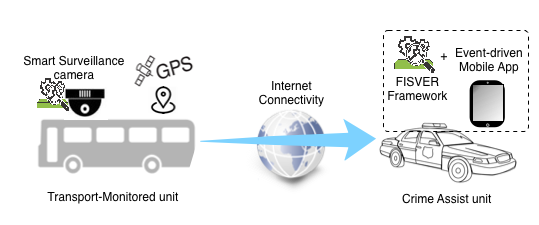
\includegraphics[scale=0.8]{Imagens/cap5_typical_testbed.png}
 	\caption{Typical Deployment testbed configuration}
 	\label{fig:tydep}
\end{figure}

On the one side, the Typical Deployment set of experiments aims to represent configuration sets regularly used in smart surveillance assessments for transportation-safety systems, following guidelines used in \cite{Typtest1}. For this dissertation, the configuration of the Typical Deployment set of experiments consider in-vehicle video surveillance subsystems sensing the cabin surroundings, and permanently streaming corresponding video flow towards a pre-assigned mobile application, leveraging available Internet connectivity. At the mobile application side, a video processing application using the Haar Cascade Features \cite{peng2011}, is in charge to process analytics on the received video streaming to detect objects and infer crime events. If any crime object matching is achieved, an alert event is dispatched to the notification area, so that reporting the user at the mobile device screen. The FISVER Built-in set of experiments is depicted in the Figure\ref{fig:fradep}.

\begin{figure}[!htb]'
	\centering
 	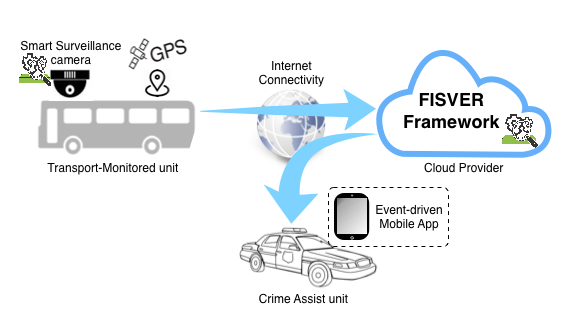
\includegraphics[scale=0.8]{Imagens/cap5_fisver_testbed.png}
 	\caption{FISVER Built-in testbed configuration}
 	\label{fig:fradep}
\end{figure}

On the other side, the FISVER Built-in set of experiments is in charge to prototyping the main subject of this dissertation. The configuration of the FISVER Built-in set of experiments is in compliance with the specifications detailed in the Chapter 4. In this set of experiments, the in-vehicle smart surveillance subsystem keeps constantly sensing the bus cabin surroundings, and uses the Haar Cascade Features to detect target crime objects locally. On detecting an object of potential security threat, the FISVER agent inside the camera composes a corresponding metadata set containing indication of the crime occurrence, GPS location of the vehicle and an image to sample the crime occurrence. Afterwards, it uses onboard Internet connectivity to send the metadata towards the cloud infrastructure featuring the FISVER approach. At the cloud, FISVER inspects the metadata to classify the indicated event. On confirming the crime event, it uses the derived GPS location to find in local data base the best crime assist. On the basis of finding the best crime assist unit, cloud FISVER in turn extends the corresponding metadata with the crime event classification, and sends it to the crime assist unit. 

To ensure that a similar processing deployment and comparative equality are maintained, the image processing algorithms are deployed in a Java\footnote[20]{Java. https://www.java.com/en/. Accessed on December 12th, 2015.} virtual machine that is called C++\footnote[21]{C++. http://www.cplusplus.com/. Accessed on December 12th, 2015.} native library. This was designed with aid of OpenCV\footnote[22]{OpenCV. http://opencv.org/. Accessed on December 12th, 2015.} , to create image manipulations and deploy the haar cascade feature algorithm. 

A Typical NDK\footnote[23]{NDK. http://developer.android.com/ndk/index.html. Accessed on December 12th, 2015.} Scenario is used to make native library loading for the Android mobile application. The native library loads are made through JNI for the FISVER Built-in set of experiments.

\section{Methodology applied for the Assessments}

Four tests are assigned for each one of the set of experiments, with the perspective to allow examining the impact in the testbed behavior under different conditions imposed by varying rates of notification load that is offered to the system \cite{Evaluation2}. Before conducting the target experiments, the testbed was stressed with an amount of crime detect notifications from smart surveillance camera. The goal is to figure out the maximum capacity of the system in handling security notifications without crashing it \cite{Evaluation4}, for use as benchmarking reference. The stressing test reveals a load of 3,600 offered security notification, which were sent out during the period of one hour of the experimental time.

In order to ease the prototype experimentation, the in-vehicle smart surveillance based transportation-safety system is represented by a software application that generates a number of notifications over the course of their experimental time (i.e., one hour) following the poison distribution, similarly as in \cite{Evaluation3}. Four datasets are deployed, each with a variation in the number of security notifications in function of the total security notifications set (i.e.,  3,600), allowing following workloads: 30\% (1,080 notifications), 60\% (2,160 notifications), 90\% (3,240 notification) and 120\% (4,320 notification). 

\section{Result Analysis}

On the basis that cloud-enabled smart surveillance based transportation-safety systems have critical performance issues, it is fundamental to adopt accurate benchmarking for obtaining consistent insights in multiple dimensions of resource consumption and optimization rates\cite{Evaluation5}. For the benchmarking model, the decision is to concentrate in the mobile device performance parameters, which is justified by the need on  obtaining insights in the perspective of the most agility demanding subsystem in the framework, the crime assist unit which will deal on the crime at the end.  

Assessments in the performance aspects at both in-vehicle and cloud FISVER subsystems are interesting and relevant, at the end the performance in the mobile unit brings the concrete view in overall interworking operations and user experience. Average rates in CPU utilization load, download/upload throughput and battery consumption on the event-driven mobile application side for the two set of experiments, are used as key performance information. To understand the behavior characteristics resulting from the surveillance system’s configurations, the benchmarking considers analysis in the runtime statistics collected while running the applications on the four workloads corresponding to each set of experiments. Each experiment is repeated 10 times, whereby averaging results are plotted to produce graphs, considering a confidence interval of 95\%.

\subsection{CPU Load Analytics}
\label{CPUAnalytics}

In regards to cloud-enabled Smart Surveillance systems, the list of major concerns facing these systems include scalability, ubiquitous access to sensory data, event processing overhead, and massive storage requirements \cite{Anwar_Hossain}. All of them together demand optimized service approach, and thus CPU utilization load is an important measure to estimate effectiveness on system performance. The CPU load analytics envisages to studying the utilization rate that both FISVER Built-in and Typical Deployment features take to the mobile device in the testbed with the varying offered notification load. The results of the CPU load obtained in both experiments are shown in Figure \ref{fig:result2}.

\begin{figure}[htb]
	\centering
 	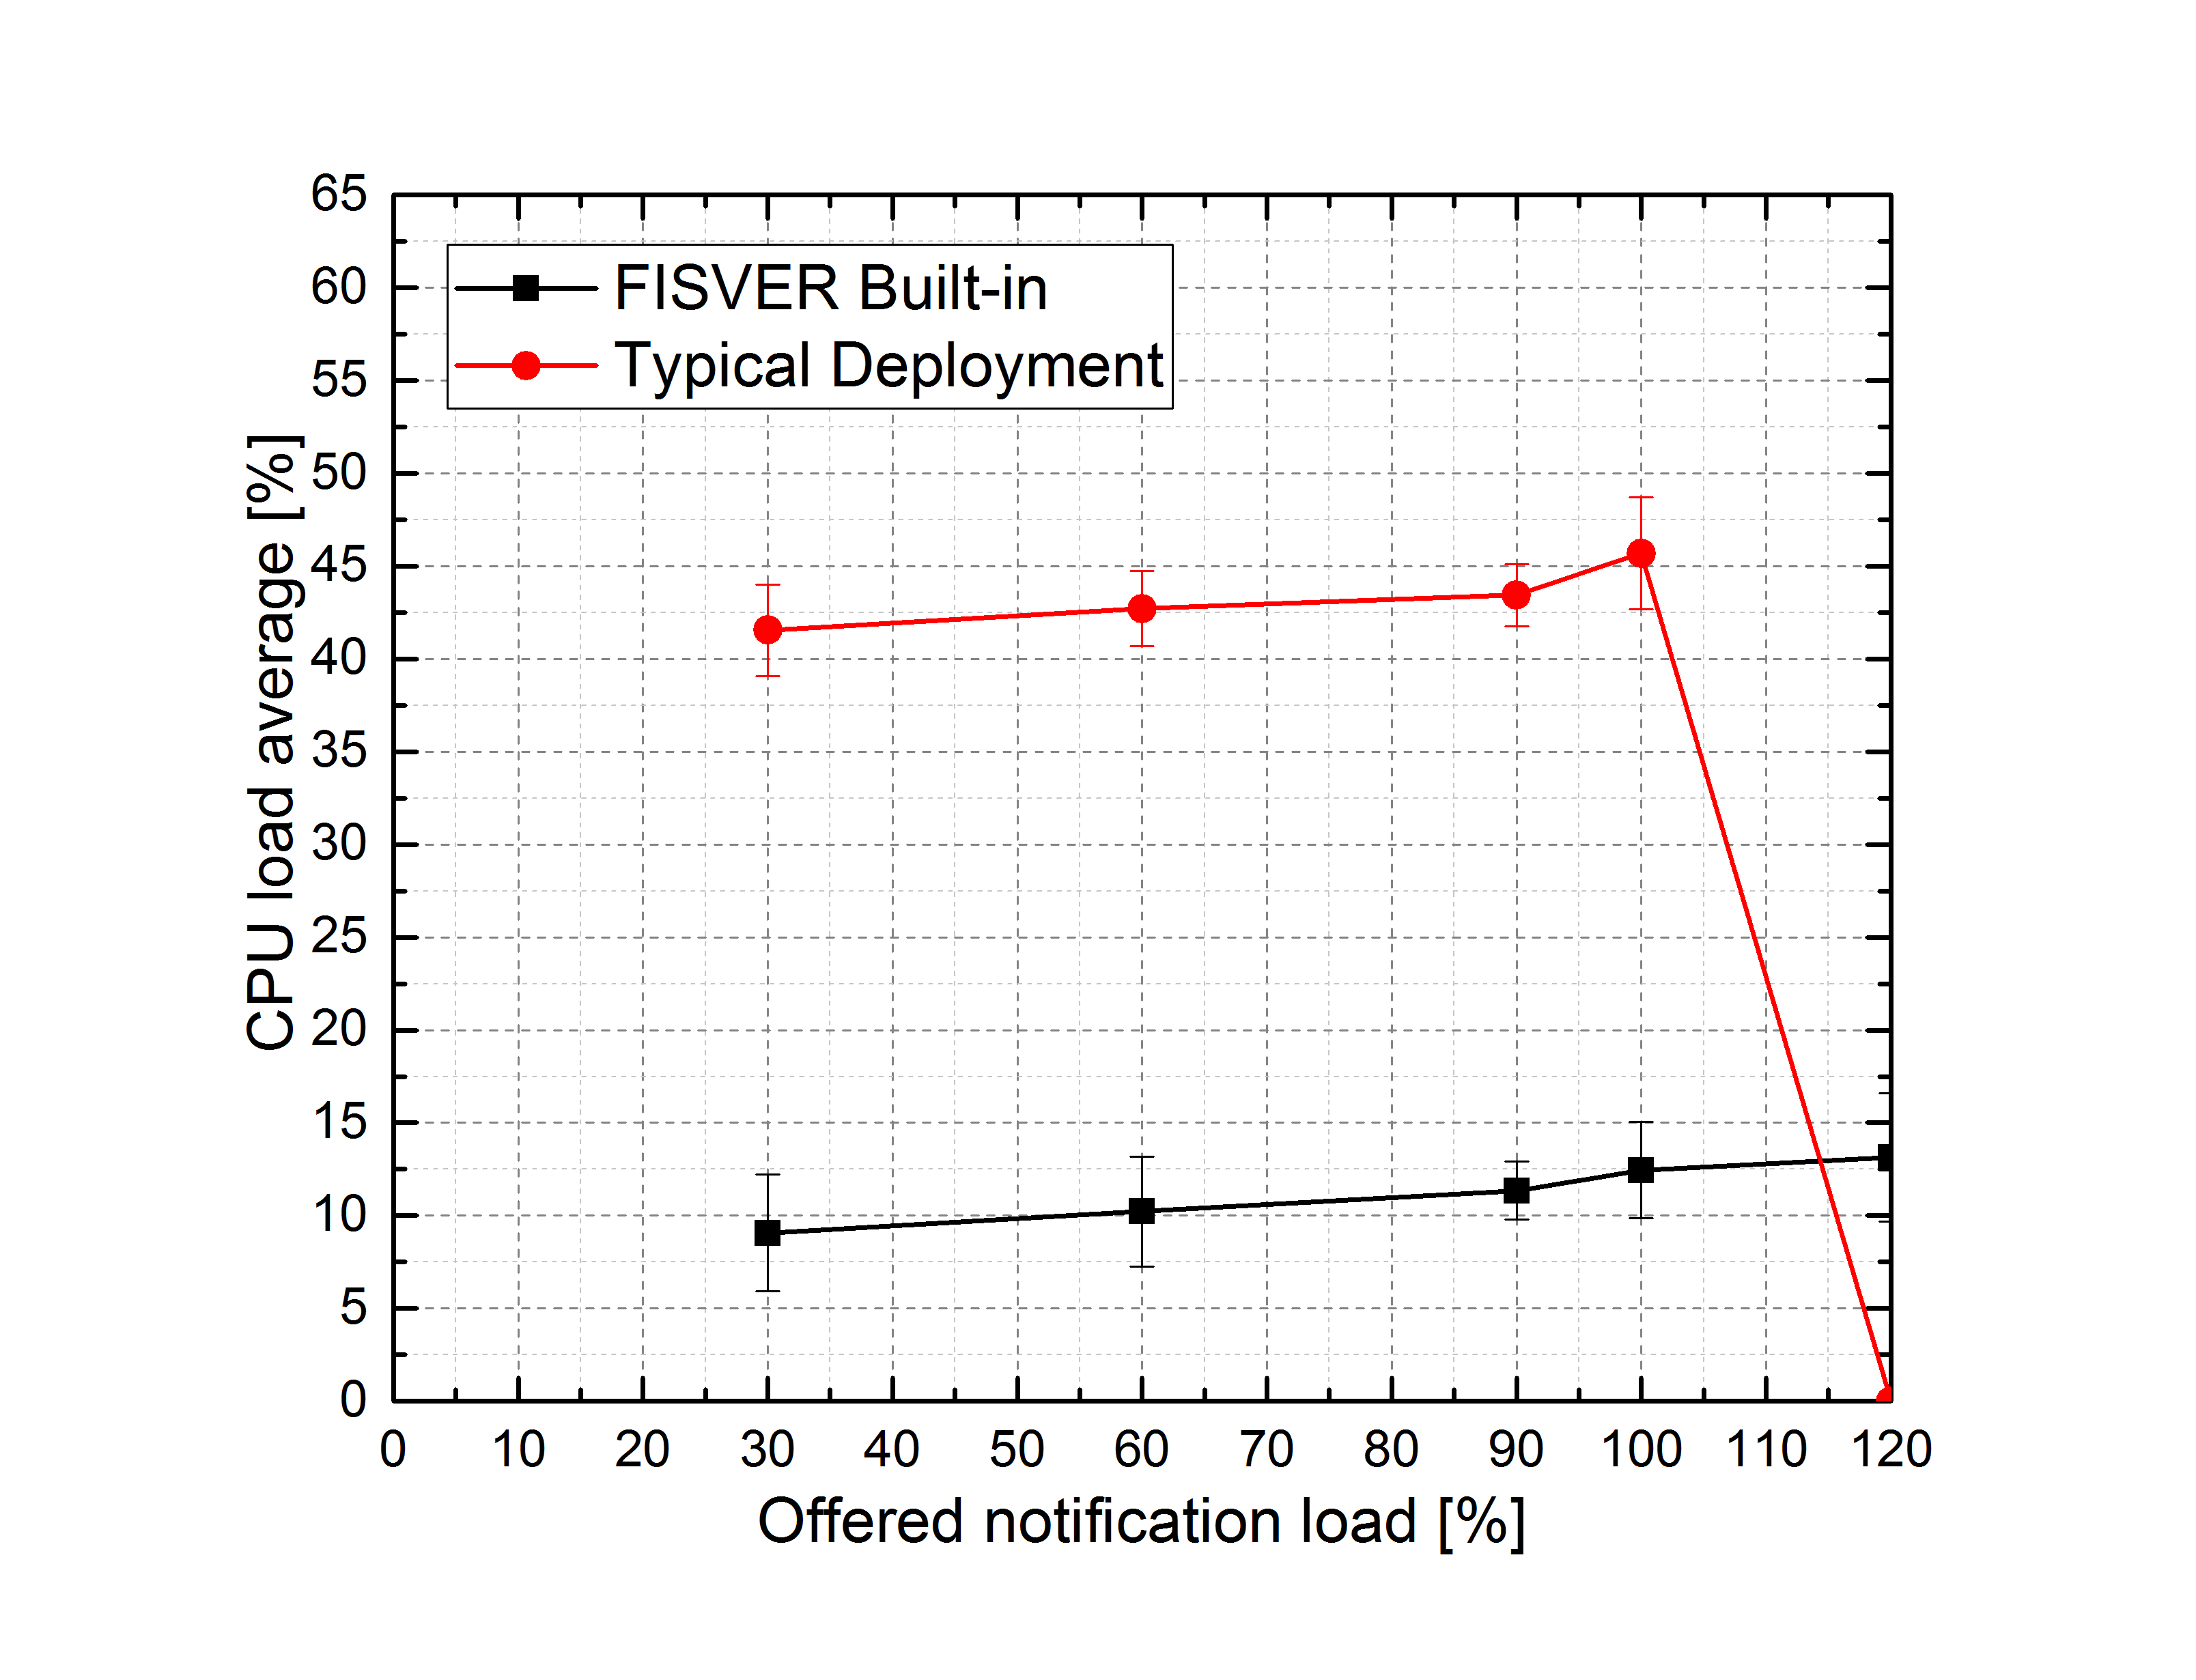
\includegraphics[scale=0.60]{Imagens/cap5_cpu.png}
 	\caption{CPU average load.}
 	\label{fig:result2}
\end{figure}

The results scratched in Figure \ref{fig:result2} confirm that the number of instances significantly affects the CPU consumption, which increases exponentially with the offered notification load scale. This behavior can be explained by the need to report the event-driven mobile application whenever the cloud service classifies a potential crime threat. Thus, the more target notifications are produced, the more crime event reports are generated and sent to the event-driven mobile application. The averaging CPU consumption in the FISVER Built-in set of experiments is of 10.94\%, whereas 44.84\% in the Typical Deployment testbed configuration. Thus, the results reveal that FISVER allows improving the CPU performance around 75.6\%.

The main reason for this improvement is obtained through the FISVER assistance, whereby all the Smart Surveillance complex tasks are carried out by both in-vehicle and cloud interworking subsystems, leaving the event-driven mobile application mostly in charge only to present the notification to the user. It is important to highlight that the Typical Deployment is unable to achieve the end of the experiments when submitted to 120\% of the offered notification load, because the system freezes by processing overload.

\subsection{Network Bandwidth Analytics}
\label{NetAnalytics}

The analysis in networking behavior has as main objective to observe the impact that the FISVER proposal takes in transport resources from the underlying intercommunication system. This set of analysis play a key role in estimating the system scalability, since networking imposes challenges and issues with regard to QoE, responsiveness, cost and survivability, specially in resource constrained mobile devices. For that, bandwidth consumption rates during both downstream (i.e., infrastructure/in-vehicle system to mobile app) and upstream (i.e., mobile app to infrastructure/in-vehicle system) service transport utilization are collected as measures for performance analysis across the different offered notification load. Figure (\ref{fig:result3}) illustrates the results in upload networking bandwidth utilization. 

\begin{figure}[htb]
	\centering
 	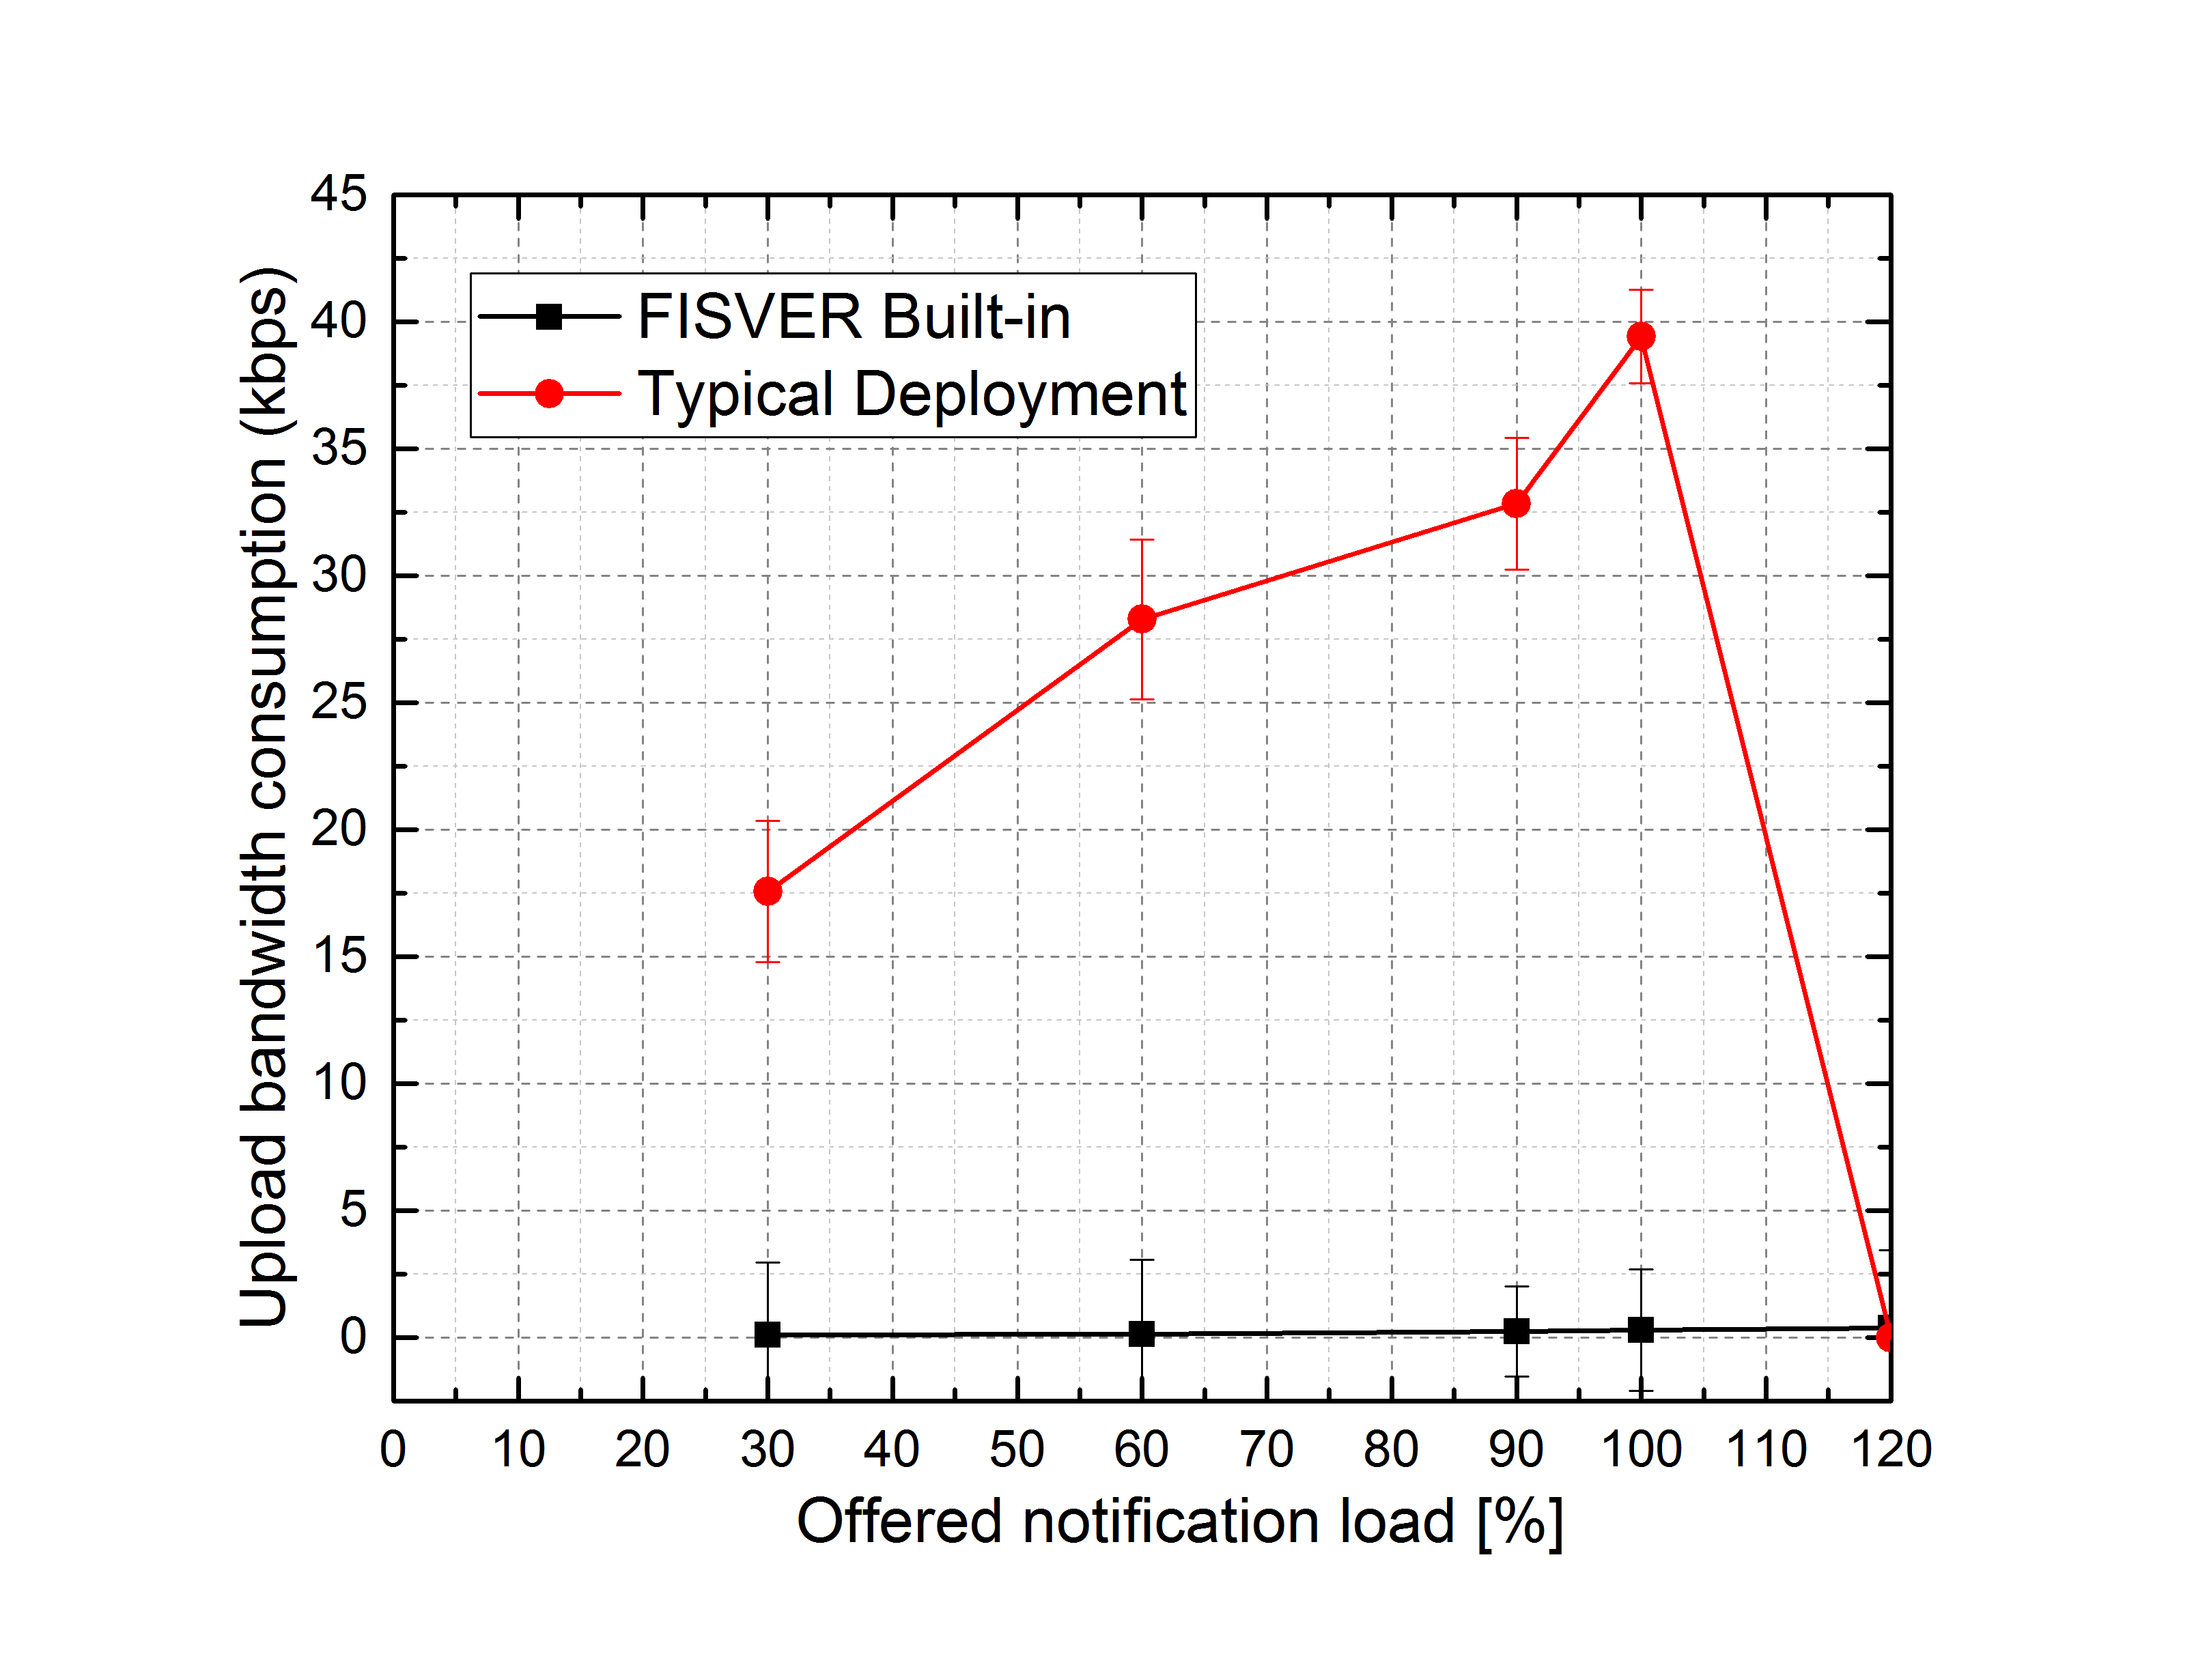
\includegraphics[scale=0.60]{Imagens/cap5_upload.png}
 	\caption{Upload bandwidth consumption.}
 	\label{fig:result3}
\end{figure}

As it can be observed in the Figure \ref{fig:result3}, the FISVER approach allows allocating around 0.2 kbps (i.s., less than 0.0018\% of the overall available bandwidth capacity) at the upstream service transport in the course of the experiments. On another hand, the Typical Deployment testbed configuration allocates an average of 29.53 kbps (26\%), therefore demonstrating an outstanding networking performance improvement of 99.993\%. This is achieved by concentrating all heavyweight processing task at the infrastructure, thus leaving the smartphone lightweight because the in-vehicle processing algorithm only dispatches crime events detections upon obtaining a positive target matching. Figure \ref{fig:result4} shows the average networking behavior in the downstream transport service during FISVER Built-in and Typical Deployment set of experiments.

\begin{figure}[htb]
	\centering
 	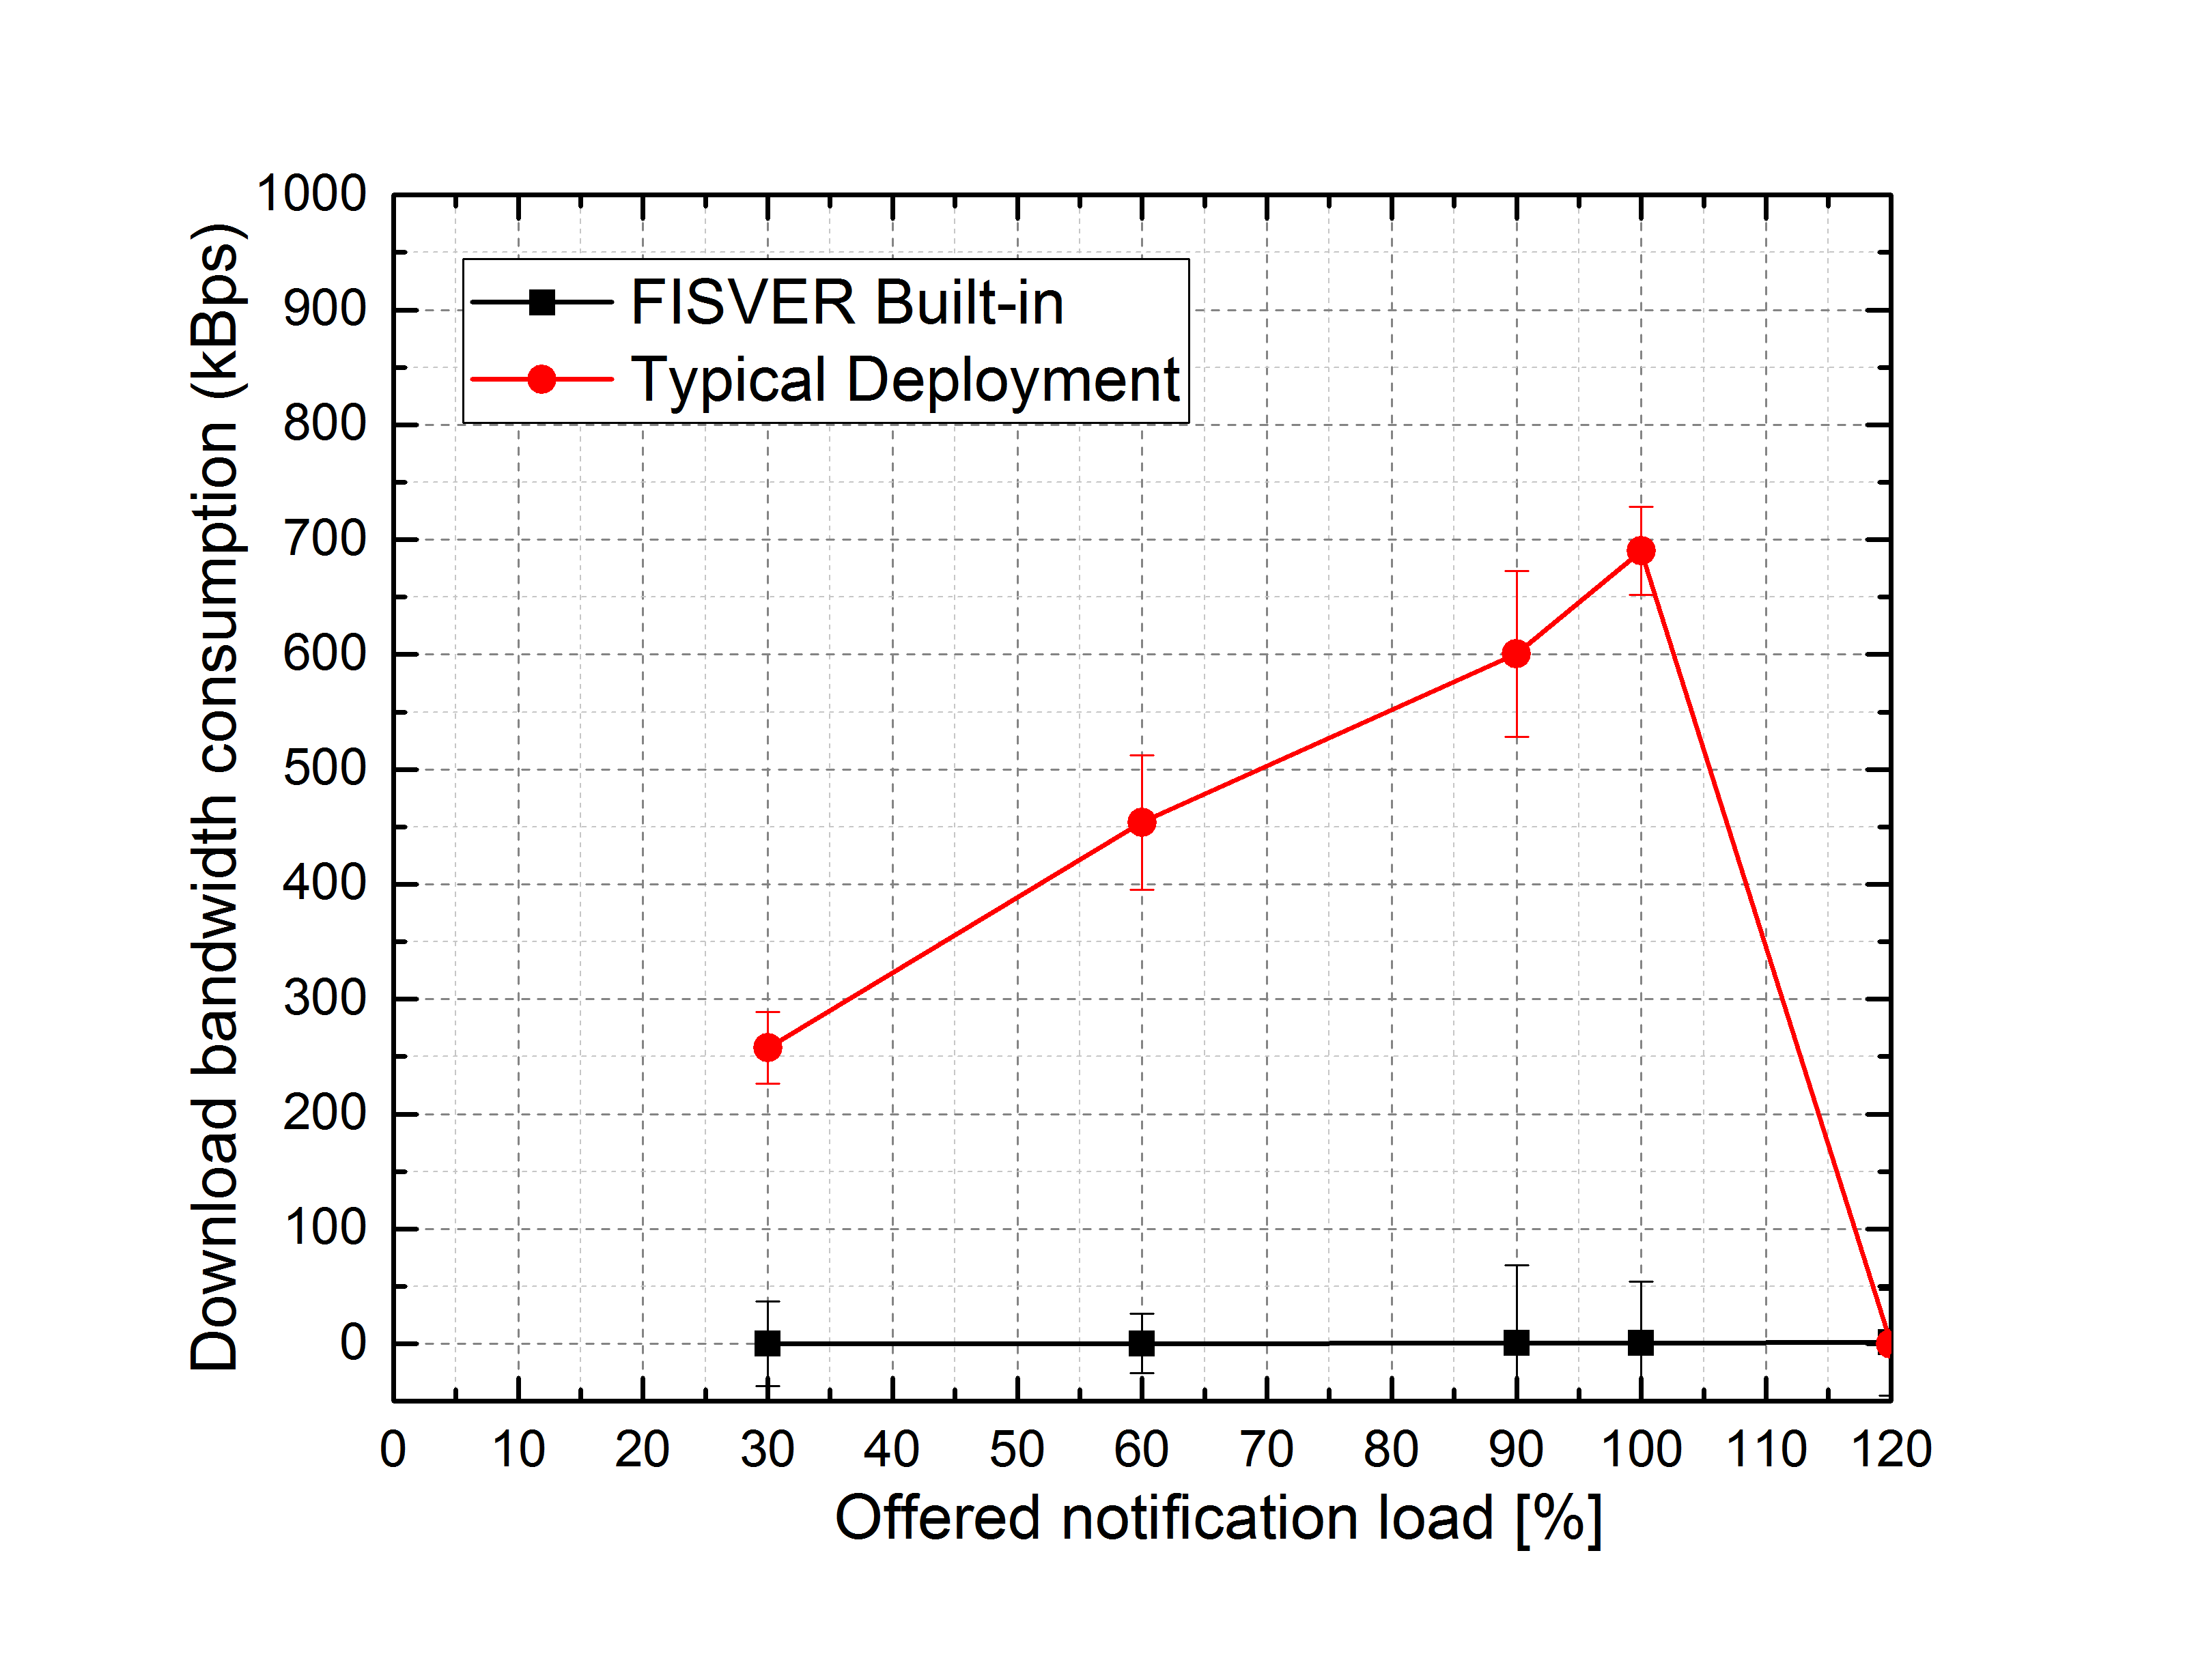
\includegraphics[scale=0.60]{Imagens/cap5_download.png}
 	\caption{Download bandwidth consumption.}
 	\label{fig:result4}
\end{figure}

In regards to the bandwidth utilization rate for the procedures using downstream service transport, Figure \ref{fig:result4} reveals that an insignificant variation exists in the behavior of the event-driven mobile application at the FISVER Built-in, averaging 0.52 kbps (0.004\% of the overall bandwidth capacity). In the opposite, the Typical Deployment set exhibits an average 512 kbps of networking demand during the experiments, with exponential increasing behavior for the utilization of the downstream network link. The networking behavior in the Typical Deployment set is justified by it's design approach that pushes to the mobile application the task for deploying all the complex processing procedures, as well as user notification. Therefore, the downstream networking performance in FISVER Built-in set of experiments dramatically outperforms the Typical Deployment results by around 99,998\%. It is important to highlight similar networking improvement performance at both upstream and downstream transport services that are allowed by the FISVER approach, which demonstrates very low resource demands in comparison to the Typical Deployment set.

The impact in the device survivability that both FISVER Built-in and Typical Deployment take in the experiments is estimated by observing the  energy consumption behavior, which is considered in the next section. 

\subsection{Battery Consumption Analytics}
\label{BatAnalytics}

Device survivability is an essential aspect for reliable services, specially on mission critical use cases which requires service continuity. Service disruption by mission critical factors will result in serious impact on the target environment. In this dissertation's field of study, the impacts in safety threats in transportation service can cause social turmoil, accidents and even deaths, which is totally unacceptable and must be avoided at any cost.

The benefits of mobile computing includes ubiquitous access to the Internet, but significantly challenges survivability due to the severe battery consumption that mobile devices consume to keep wireless connectivity and service continuity. Therefore, energy consumption is a key performance measure for benchmarking cloud-enabled Smart Surveillance systems, allowing to reveal the capability that a mobile device affords in keeping available and accessible itself during processing tasks beyond mobility communications.

For this set of analysis, the battery consumption is measured in both testbed configurations over the evaluation time, with the goal to observe the impact of the FISVER approach over the Typical Deployment set of experiments on the energy sustainability of the mobile device when running the event-driven mobile application. The results obtained are scratched in Figure \ref{fig:result1}.

\begin{figure}[htb]
	\centering
 	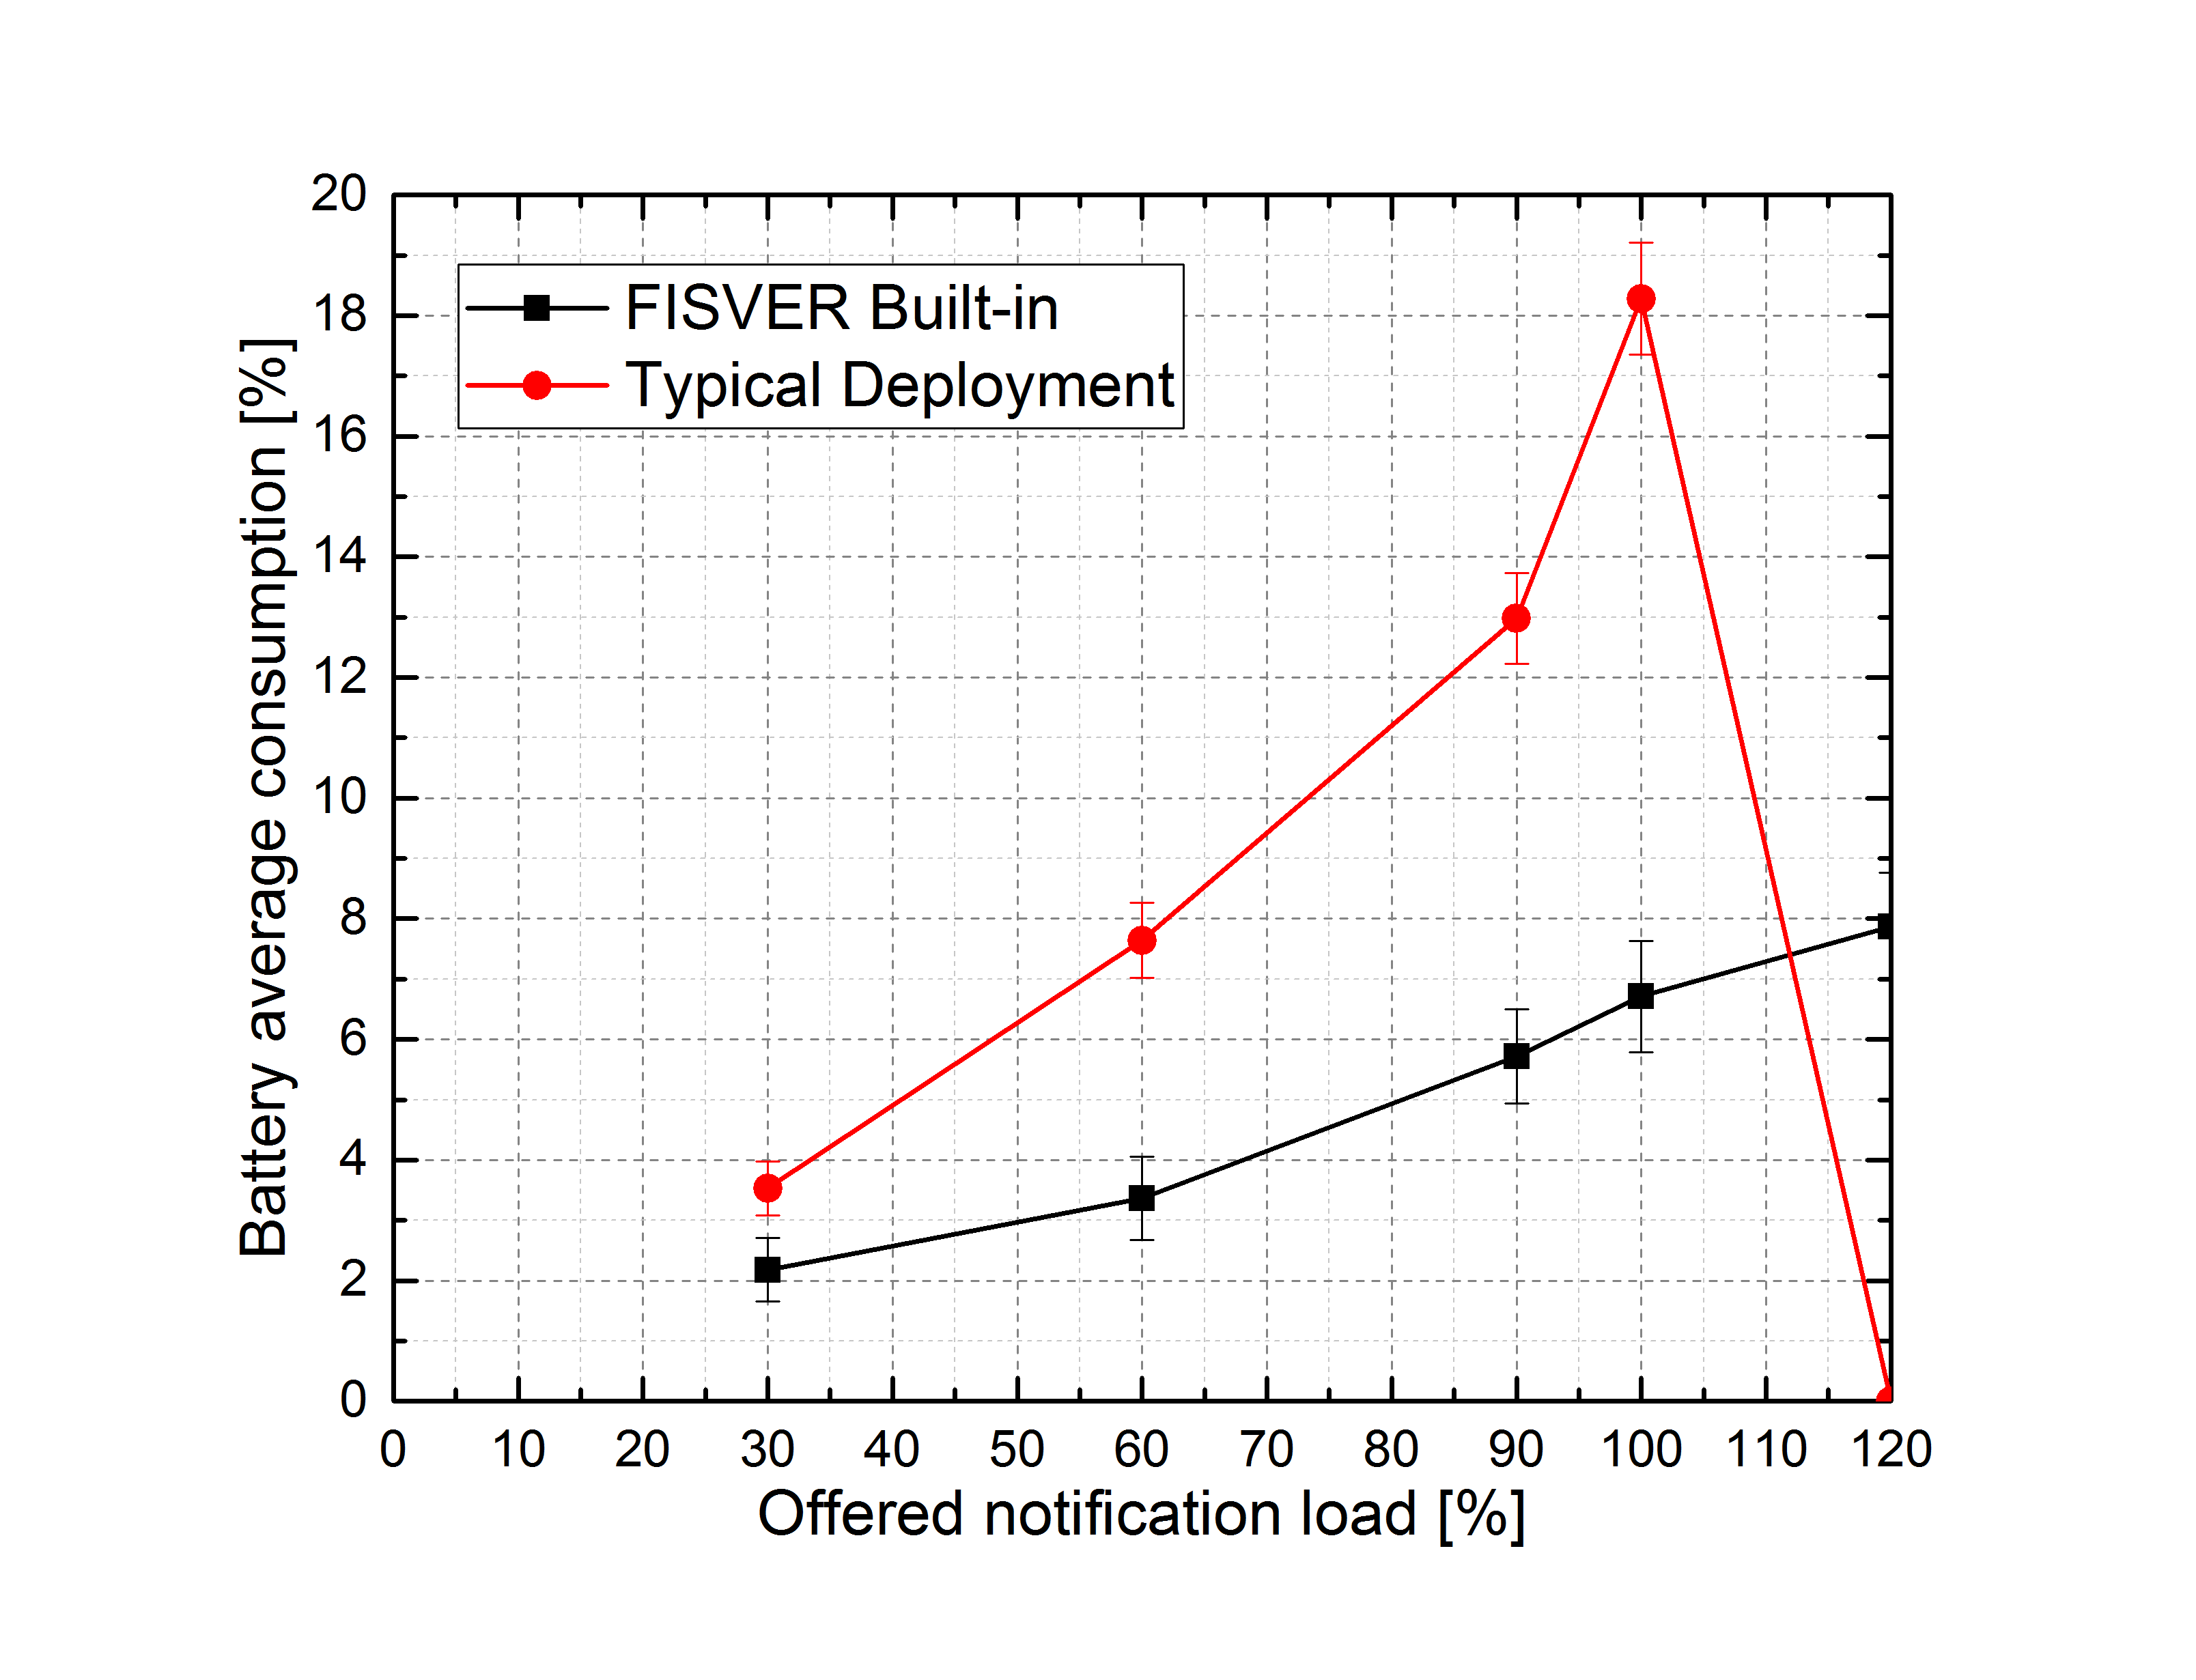
\includegraphics[scale=0.60]{Imagens/cap5_bat.png}
 	\caption{Average battery power consumption in FISVER Built-in and Typical Deployment set of experiments}
 	\label{fig:result1}
\end{figure}

As it can be confirmed from the results scratched by Figure \ref{fig:result1}, the percentage of the energy that is consumed in the Typical Deployment set of experiments follows the same behavior as for both \ref{NetAnalytics} and \ref{CPUAnalytics} in respect to exponential projection with the increasing offered event notification load. This behavior follows the same reasons as for those previous analysis, on the basis that the mobile application side deploys heavyweight processing tasks, whereas a lightweight event-driven approach is provisioned at the FISVER Built-in testbed.

The outcomes analytics expose that FISVER Built-in outperforms the Typical Deployment set of experiments by achieving an average battery consumption performance of 99.54\% (from 4,88\% to 10,61\% respectively). Therefore, this experiment set has proven that streaming-based mobile applications of Typical Deployment scenario is not energy-efficient over the FISVER Built-in approach, by the need for constantly accessing the network and processing video data analytics.

\subsection{Result Analysis Insights}
\label{ResAnalyIns}

The significant improvements in the consumption rates of the battery, CPU and networking resources obtained from the FISVER Built-in set of experiments compared with the Typical Deployment configuration, are essentially explained by the influence of the notification-based cloud approach, which allows a sharp decline in the amount of resource demands at the mobile device.

While the transport safety application generally remains connected in standby mode in the FISVER Built-in set of experiments, the coupled-based approach deployed by the Transport Safety application in the Typical Deployment set of experiments requires frequent data exchanges to gather in-vehicle raw data from the remote system.

The results highlighted in this chapter on the testbed assessments, allow to demonstrate the suitability of FISVER proposal in affording cloud-enabled smart surveillance based transport-safety services, as well as its outstanding performance over the Typical Deployment experiment sets. The FISVER proposal evidences performance improvement in CPU utilization load (75.6\%), upstream(99.993\%)/downstream(99.996\%) throughput and battery consumption (99.54\%) in comparison to the behavior of the Typical Deployment set of experiments.
 	 
		
	% Consideracoes finais
	% Considerações finais
\chapter{Conclusion and Suggestions for Future Work}


This work proposes FISVER as a means of allowing the current Safety Transport systems to evolve towards the future smart Surveillance. The main motivation in doing this work is the sharp increase of crime events in Brazilian public transportation system. Several challenges was found due Brazil's mobile network limitations, otherwise, proposed framework proved to overcome them by adopting some strategies, there are:

\begin{itemize}
\item In-vehicle video processing for agile detection of targeted crime objects;
\item Image processing based event classification provisioned as a cloud service;
\item Instant crime event notification as a cloud service, to trigger the best crime assist through mobile application(s);
\item Event-driven operating support paradigm, for performance-enhanced and energy-efficient perspectives of application(s) running at crime assist mobile devices.
\end{itemize}

A review on relevant related works was done, in order to verify the relevance and contribution of the present proposal.  Basically, none of the related works are able to meet the key requirements that are claimed in this dissertation to designate an efficient smart transportation solution, for the reason that: (i) a set of smart surveillance solutions are intended to provision storage and real-time video streaming access as a cloud service, thus lacking smart computing capabilities; (ii) solutions envisioning to detect security threat events as a cloud service are based on streaming of remote surveillance cameras, thus denoting a severe bandwidth-consuming approach, costly and miss in guaranteeing QoE; lastly, (iii) the typical concentration on mobile devices to carry heavyweight smart computing features is not cost-efficient and severely affects the device performance and survivability.  All these outcomes motivate to carry out the present work, with great relevance in scientific research activity perspectives.

The FISVER proposal deploys a holistic cloud infrastructure that embodies a hub of modern services and applications that seek to provide a seamless, integrated Sensor and Transport Safety Application as a cloud service with ubiquitous access. The main benefit of FISVER is that it can alleviate the task of designing transport safety applications by deploying a notification-based approach to ensure an optimized performance and the survival of the mobile devices. Moreover, FISVER supports customized alerts to provide enhanced insights while keeping the Transport Safety applications lightweight. The FISVER  proposal features a modular architecture of components and subcomponents, that interwork to provision value-added smart procedures, and are accessible through open web-based interfaces. 

A set of experiments has been carried out following the premise to assess the suitability of the FISVER proposal in helping to detect security threats at public bus transportation use case in real-time, as well as agile calling appropriate crime assistance units. The performance evaluation considers prototyping the FISVER approach on a real tested, for accurate benchmarking. The methodology applied in the evaluation defines a Typical Smart Surveillance System Deployment, that is submitted to the same conditions as for the FISVER Built-in set of experiments. Each prototype configuration has been submitted to different notification load conditions, with benchmarking centered on the resulting experience at the mobile application side.  The benchmarking considered analysis in the runtime statistics collected while running  all set of experiments. 

The collected results indicate that FISVER achieves great improvements in regards to CPU load (75.6\%), bandwidth consumption (99.99\%) and ) energy efficiency (99.54\%) when compared to the behavior of the Typical Deployment set of experiments. The outstanding performance improvement of the FISVER approach over the Typical Deployment scenario in regards to CPU load (from 44.84\% to 10.94\%) is allowed through the effect of preventing the necessity to report the event-driven mobile application whenever the cloud service matches a potential crime threat. This way, FISVER reveals a significant event-constrained approach over the Typical Deployment configuration, which allows to optimize the networking performance at both upstream (from 0.2 kbps to 29.53 kbps) and downstream (from 512 kbps to 0.52 kbps) transport services. Finally, the lightweight event-driven approach that FISVER allows for mobile applications dramatically outperforms the streaming-based strategy of Typical Deployment use cases, with optimization rates from  10.61\% to 4.88\%. 

The results that are obtained in the evaluations demonstrate the suitability that the FISVER proposal takes over  the Typical Deployment testbed in affording cloud-enabled surveillance based transport-safety services. The assessment results reveals outstanding system performance and device survivability behaviors of FISVER over the Typical Deployment, enforcing its essential contribution in mission critical situations, with agility and efficiency. 

\section{Future Work}

The outcomes of this work raise needs for future work efforts in different fields of research, as in the following. The FISVER proposal is considered to be integrated on real security systems that are currently deployed at municipalities, in order to assess his suitability and performance. Moreover, FISVER is envisioned for use in other mission critical use cases, with the perspective to allow detecting security threats in urban areas (squares, streets, beaches, etc.), buildings/homes, and so on. Finally, privacy aspects are not under consideration by this dissertation, because the main focus is on the infrastructure and networking features. 

 % Conclusão e Trabalhos Futuros

	% Bibliografia (arquivo Capitulos/Referencias.bib)
	\bibliography{Capitulos/Referencias}
	\bibliographystyle{abnt-alf}
%	\bibliographystyle{abnt}
%	\bibliographystyle{ieeetr}
%	\bibliographystyle{unsrt}
%	\bibliographystyle{babunsrt}
%	\bibliographystyle{unsrtnat}
%	\bibliographystyle{abbrvnat}
%	\bibliographystyle{plain}
%	\bibliographystyle{babplain}
%	\bibliographystyle{babunsrt}
%	\bibliographystyle{abbrv}
	
	% Apêndice A (arquivo Includes/ApendiceA)
	%\include{Capitulos/ApendiceA}
	
	% Anexo A (arquivo Includes/AnexoA)
%	\include{Capitulos/AnexoA}
	
	% Página em branco
	\newpage

\end{document}